% This is the Reed College LaTeX thesis template. Most of the work
% for the document class was done by Sam Noble (SN), as well as this
% template. Later comments etc. by Ben Salzberg (BTS). Additional
% restructuring and APA support by Jess Youngberg (JY).
% Your comments and suggestions are more than welcome; please email
% them to cus@reed.edu
%
% See http://web.reed.edu/cis/help/latex.html for help. There are a
% great bunch of help pages there, with notes on
% getting started, bibtex, etc. Go there and read it if you're not
% already familiar with LaTeX.
%
% Any line that starts with a percent symbol is a comment.
% They won't show up in the document, and are useful for notes
% to yourself and explaining commands.
% Commenting also removes a line from the document;
% very handy for troubleshooting problems. -BTS

% As far as I know, this follows the requirements laid out in
% the 2002-2003 Senior Handbook. Ask a librarian to check the
% document before binding. -SN

%%
%% Preamble
%%
% \documentclass{<something>} must begin each LaTeX document
\documentclass[12pt,twoside,openany]{reedthesis}
% Packages are extensions to the basic LaTeX functions. Whatever you
% want to typeset, there is probably a package out there for it.
% Chemistry (chemtex), screenplays, you name it.
% Check out CTAN to see: http://www.ctan.org/
%%

\usepackage{setspace}
\usepackage{graphicx,latexsym}
\usepackage{amsmath}
\usepackage{amssymb,amsthm}
%\usepackage{longtable,booktabs,setspace}
\usepackage{longtable,booktabs,setspace, array}
\usepackage{chemarr} %% Useful for one reaction arrow, useless if you're not a chem major
\usepackage[hyphens]{url}
% Added by CII
\usepackage{hyperref}
\usepackage{lmodern}
\usepackage{float}
\floatplacement{figure}{H}
% End of CII addition
\usepackage{rotating}
% Next line commented out by CII
%%% \usepackage{natbib}
% Comment out the natbib line above and uncomment the following two lines to use the new
% biblatex-chicago style, for Chicago A. Also make some changes at the end where the
% bibliography is included.
%\usepackage{biblatex-chicago}
%\bibliography{thesis}


% Added by CII (Thanks, Hadley!)
% Use ref for internal links
\renewcommand{\hyperref}[2][???]{\autoref{#1}}
\def\chapterautorefname{Chapter}
\def\sectionautorefname{Section}
\def\subsectionautorefname{Subsection}
% End of CII addition

% Added by CII
\usepackage{caption}
\captionsetup{width=5in}
% End of CII addition

% \usepackage{times} % other fonts are available like times, bookman, charter, palatino

% Syntax highlighting #22
  \usepackage{color}
  \usepackage{fancyvrb}
  \newcommand{\VerbBar}{|}
  \newcommand{\VERB}{\Verb[commandchars=\\\{\}]}
  \DefineVerbatimEnvironment{Highlighting}{Verbatim}{commandchars=\\\{\}}
  % Add ',fontsize=\small' for more characters per line
  \usepackage{framed}
  \definecolor{shadecolor}{RGB}{248,248,248}
  \newenvironment{Shaded}{\begin{snugshade}}{\end{snugshade}}
  \newcommand{\KeywordTok}[1]{\textcolor[rgb]{0.13,0.29,0.53}{\textbf{#1}}}
  \newcommand{\DataTypeTok}[1]{\textcolor[rgb]{0.13,0.29,0.53}{#1}}
  \newcommand{\DecValTok}[1]{\textcolor[rgb]{0.00,0.00,0.81}{#1}}
  \newcommand{\BaseNTok}[1]{\textcolor[rgb]{0.00,0.00,0.81}{#1}}
  \newcommand{\FloatTok}[1]{\textcolor[rgb]{0.00,0.00,0.81}{#1}}
  \newcommand{\ConstantTok}[1]{\textcolor[rgb]{0.00,0.00,0.00}{#1}}
  \newcommand{\CharTok}[1]{\textcolor[rgb]{0.31,0.60,0.02}{#1}}
  \newcommand{\SpecialCharTok}[1]{\textcolor[rgb]{0.00,0.00,0.00}{#1}}
  \newcommand{\StringTok}[1]{\textcolor[rgb]{0.31,0.60,0.02}{#1}}
  \newcommand{\VerbatimStringTok}[1]{\textcolor[rgb]{0.31,0.60,0.02}{#1}}
  \newcommand{\SpecialStringTok}[1]{\textcolor[rgb]{0.31,0.60,0.02}{#1}}
  \newcommand{\ImportTok}[1]{#1}
  \newcommand{\CommentTok}[1]{\textcolor[rgb]{0.56,0.35,0.01}{\textit{#1}}}
  \newcommand{\DocumentationTok}[1]{\textcolor[rgb]{0.56,0.35,0.01}{\textbf{\textit{#1}}}}
  \newcommand{\AnnotationTok}[1]{\textcolor[rgb]{0.56,0.35,0.01}{\textbf{\textit{#1}}}}
  \newcommand{\CommentVarTok}[1]{\textcolor[rgb]{0.56,0.35,0.01}{\textbf{\textit{#1}}}}
  \newcommand{\OtherTok}[1]{\textcolor[rgb]{0.56,0.35,0.01}{#1}}
  \newcommand{\FunctionTok}[1]{\textcolor[rgb]{0.00,0.00,0.00}{#1}}
  \newcommand{\VariableTok}[1]{\textcolor[rgb]{0.00,0.00,0.00}{#1}}
  \newcommand{\ControlFlowTok}[1]{\textcolor[rgb]{0.13,0.29,0.53}{\textbf{#1}}}
  \newcommand{\OperatorTok}[1]{\textcolor[rgb]{0.81,0.36,0.00}{\textbf{#1}}}
  \newcommand{\BuiltInTok}[1]{#1}
  \newcommand{\ExtensionTok}[1]{#1}
  \newcommand{\PreprocessorTok}[1]{\textcolor[rgb]{0.56,0.35,0.01}{\textit{#1}}}
  \newcommand{\AttributeTok}[1]{\textcolor[rgb]{0.77,0.63,0.00}{#1}}
  \newcommand{\RegionMarkerTok}[1]{#1}
  \newcommand{\InformationTok}[1]{\textcolor[rgb]{0.56,0.35,0.01}{\textbf{\textit{#1}}}}
  \newcommand{\WarningTok}[1]{\textcolor[rgb]{0.56,0.35,0.01}{\textbf{\textit{#1}}}}
  \newcommand{\AlertTok}[1]{\textcolor[rgb]{0.94,0.16,0.16}{#1}}
  \newcommand{\ErrorTok}[1]{\textcolor[rgb]{0.64,0.00,0.00}{\textbf{#1}}}
  \newcommand{\NormalTok}[1]{#1}

% To pass between YAML and LaTeX the dollar signs are added by CII
\title{Regime Detection Measures for the Practical Ecologist}
\author{Jessica L. Burnett}
% The month and year that you submit your FINAL draft TO THE LIBRARY
\date{2019}
\division{}
\advisor{Craig R. Allen}
\institution{University of Nebraska-Lincoln}
\degree{Doctor of Philosophy}
%If you have two advisors for some reason, you can use the following
% Uncommented out by CII
\altadvisor{Dirac Twidwell}
% End of CII addition

%%% Remember to use the correct department!
\department{School of Natural Resources}
% if you're writing a thesis in an interdisciplinary major,
% uncomment the line below and change the text as appropriate.
% check the Senior Handbook if unsure.
%\thedivisionof{The Established Interdisciplinary Committee for}
% if you want the approval page to say "Approved for the Committee",
% uncomment the next line
%\approvedforthe{Committee}

% Added by CII
%%% Copied from knitr
%% maxwidth is the original width if it's less than linewidth
%% otherwise use linewidth (to make sure the graphics do not exceed the margin)
\makeatletter
\def\maxwidth{ %
  \ifdim\Gin@nat@width>\linewidth
    \linewidth
  \else
    \Gin@nat@width
  \fi
}
\makeatother

\renewcommand{\contentsname}{Table of Contents}
% End of CII addition

\setlength{\parskip}{0pt}

% Added by CII

\providecommand{\tightlist}{%
  \setlength{\itemsep}{0pt}\setlength{\parskip}{0pt}}

\Acknowledgements{
Graduate school itself isn't hard, but the journey is. I have a lot of
people and institutions to thank for their emotional, intellectual,
financial, and other support. I wish to first highlight how
\textbf{great it was to be a graduate student at this university and in
the School of Natural Resources}. UNL has provided tremendous support at
all levels of the university. Although I am not a fan of Nebraska's
climate, I highly recommend this school to prospective students. I thank
my supervisors, Craig Allen and Dirac Twidwell, for providing me with
this amazing opportunity and for supporting my growth as an independent
researcherm and my committee members, Craig Allen, David Angeler, John
De Long, Dirac Twidwell, and Drew Tyre for their support and advisement,
but especially for their comprehensive examination--I found this process
transformative, albeit very stress inducing. I also wish to thank Dirac
for his comprehensive exam questions--I never knew how much I didn't
know until I studied your recommendations. I also thank Craig for
supporting my efforts to study and conduct research outside of our
immediate geographical settings. Studying at the International Institute
for Applied Systems Analysis was an amazing opportunity! I thank Brian
Fath and Elena Rovenskaya for their advisement, members of the Applied
Systems Analysis research group for their feedback on my research, and
to the postdocs and YSSPers. I would like to especially thank some of
the amazing and brilliant \textbf{female scientists} in my life for
their encouragement: Jane Anderson, Karen Bailey, Hannah Birge, Mary
Bomberger Brown, Tori Donovan, Brittany Dueker, Allie Schiltmeyer, Katie
Sieving, Erica Stuber, Becky Wilcox, Carissa Wonkka, and Lyndsie Wszola.
I thank these women and others for their contributions to my
professional development: David Angeler, Christie Bahlai, Mary Bomberger
Brown, John Carroll, Jenny Dauer, John DeLong, Tarsha Eason, Brian Fath,
Ahjond Garmestani, Chris Lepczyk, Frank La Sorte, Chai Molina, Zac
Warren, Hao Ye and Peter Zebrowski. I owe thanks to Craig Allen and
Kevin Pope for entertaining my many hours of discussion (interrogation?)
regarding federal employment. I also thank fellow graduate students whom
I hope I have forged strong and lasting connections: Hannah Birge, Tori
Donovan, Caleb Roberts, Allie Schiltmeyer, and Lyndsie Wszola I am one
of the many graduate students afflicted with mental health
``disorders''. I am first grafteful to one friend (H) who unknowingly
destigmatized mental health in my mind and wihtout whom I may not have
sought treatment. I applaud students and faculty who have been outspoken
regarding mental health related issues, and I am indebtted to my general
practitioner and mental health advocate, Terry Thomas M.A., M.S.N.,
A.P.R.N.\\
\emph{Financial support}. This research was funded by the U.S.
Department of Defense's Strategic Environmental Research and Development
Program (project ID: RC-2510). The University of Nebraska-Lincoln (UNL)
has been highy supportive in my doctoral studies and reserach. I am
grateful for the generous of donors to the University of Nebraska
Foundation, which provided me with two prestigious supplemental
fellowships: Fling and Othmer. I also thank the Nelson Family (Nelson
Memorial Fellowship) and the Institute of Agriculture and Natural
Resources, who funded large portions of my academic and research-related
travel. I thank the School of Natural Resources for their financial
support in my conference travel. The U.S. National Academy of Sciences
generously funded part of my travel to the International Institute for
Applied Systems Analysis (IIASA). This financial support provided me not
only with invaluabe opportunities to attend and present at national and
international conferences and workshops, conduct research abroad, and
network--this funding alleviated some financial pressures associated
with graduate school which allowed a more refined focus on my
dissertation research. The opportunities and experiences provided to me
by each funding source were amazing, thank you. Finally, to my partner
of eight years--Schultzie--thank you for everything. Just kidding, thank
you, Nat Price, you are amazing.
}

\Dedication{
To the end-users and researchers frustrated with jargon and lack of
practical utility of ecological models and metrics. And to Mike Moulton,
without whose support and encouragement many years ago two advanced
degrees would likely not have been possible.
}

\Preface{

}

\Abstract{

}

% End of CII addition
%%
%% End Preamble
%%
%
\begin{document}

% Everything below added by CII
  \maketitle

\frontmatter % this stuff will be roman-numbered
\pagestyle{empty} % this removes page numbers from the frontmatter
  \begin{acknowledgements}
    Graduate school itself isn't hard, but the journey is. I have a lot of
    people and institutions to thank for their emotional, intellectual,
    financial, and other support. I wish to first highlight how
    \textbf{great it was to be a graduate student at this university and in
    the School of Natural Resources}. UNL has provided tremendous support at
    all levels of the university. Although I am not a fan of Nebraska's
    climate, I highly recommend this school to prospective students. I thank
    my supervisors, Craig Allen and Dirac Twidwell, for providing me with
    this amazing opportunity and for supporting my growth as an independent
    researcherm and my committee members, Craig Allen, David Angeler, John
    De Long, Dirac Twidwell, and Drew Tyre for their support and advisement,
    but especially for their comprehensive examination--I found this process
    transformative, albeit very stress inducing. I also wish to thank Dirac
    for his comprehensive exam questions--I never knew how much I didn't
    know until I studied your recommendations. I also thank Craig for
    supporting my efforts to study and conduct research outside of our
    immediate geographical settings. Studying at the International Institute
    for Applied Systems Analysis was an amazing opportunity! I thank Brian
    Fath and Elena Rovenskaya for their advisement, members of the Applied
    Systems Analysis research group for their feedback on my research, and
    to the postdocs and YSSPers. I would like to especially thank some of
    the amazing and brilliant \textbf{female scientists} in my life for
    their encouragement: Jane Anderson, Karen Bailey, Hannah Birge, Mary
    Bomberger Brown, Tori Donovan, Brittany Dueker, Allie Schiltmeyer, Katie
    Sieving, Erica Stuber, Becky Wilcox, Carissa Wonkka, and Lyndsie Wszola.
    I thank these women and others for their contributions to my
    professional development: David Angeler, Christie Bahlai, Mary Bomberger
    Brown, John Carroll, Jenny Dauer, John DeLong, Tarsha Eason, Brian Fath,
    Ahjond Garmestani, Chris Lepczyk, Frank La Sorte, Chai Molina, Zac
    Warren, Hao Ye and Peter Zebrowski. I owe thanks to Craig Allen and
    Kevin Pope for entertaining my many hours of discussion (interrogation?)
    regarding federal employment. I also thank fellow graduate students whom
    I hope I have forged strong and lasting connections: Hannah Birge, Tori
    Donovan, Caleb Roberts, Allie Schiltmeyer, and Lyndsie Wszola I am one
    of the many graduate students afflicted with mental health
    ``disorders''. I am first grafteful to one friend (H) who unknowingly
    destigmatized mental health in my mind and wihtout whom I may not have
    sought treatment. I applaud students and faculty who have been outspoken
    regarding mental health related issues, and I am indebtted to my general
    practitioner and mental health advocate, Terry Thomas M.A., M.S.N.,
    A.P.R.N.\\
    \emph{Financial support}. This research was funded by the U.S.
    Department of Defense's Strategic Environmental Research and Development
    Program (project ID: RC-2510). The University of Nebraska-Lincoln (UNL)
    has been highy supportive in my doctoral studies and reserach. I am
    grateful for the generous of donors to the University of Nebraska
    Foundation, which provided me with two prestigious supplemental
    fellowships: Fling and Othmer. I also thank the Nelson Family (Nelson
    Memorial Fellowship) and the Institute of Agriculture and Natural
    Resources, who funded large portions of my academic and research-related
    travel. I thank the School of Natural Resources for their financial
    support in my conference travel. The U.S. National Academy of Sciences
    generously funded part of my travel to the International Institute for
    Applied Systems Analysis (IIASA). This financial support provided me not
    only with invaluabe opportunities to attend and present at national and
    international conferences and workshops, conduct research abroad, and
    network--this funding alleviated some financial pressures associated
    with graduate school which allowed a more refined focus on my
    dissertation research. The opportunities and experiences provided to me
    by each funding source were amazing, thank you. Finally, to my partner
    of eight years--Schultzie--thank you for everything. Just kidding, thank
    you, Nat Price, you are amazing.
  \end{acknowledgements}

  \hypersetup{linkcolor=black}
  \setcounter{tocdepth}{2}
  \tableofcontents

  \listoftables

  \listoffigures

  \begin{dedication}
    To the end-users and researchers frustrated with jargon and lack of
    practical utility of ecological models and metrics. And to Mike Moulton,
    without whose support and encouragement many years ago two advanced
    degrees would likely not have been possible.
  \end{dedication}
\mainmatter % here the regular arabic numbering starts
\pagestyle{fancyplain} % turns page numbering back on
\doublespacing{} % Trying to set spacing between lines in body

\chapter*{Abstract}\label{abstract}
\addcontentsline{toc}{chapter}{Abstract}

Sed ut perspiciatis unde omnis iste natus error sit voluptatem
accusantium doloremque laudantium, totam rem aperiam, eaque ipsa quae ab
illo inventore veritatis et quasi architecto beatae vitae dicta sunt
explicabo. Nemo enim ipsam voluptatem quia voluptas sit aspernatur aut
odit aut fugit, sed quia consequuntur magni dolores eos qui ratione
voluptatem sequi nesciunt. Neque porro quisquam est, qui dolorem ipsum
quia dolor sit amet, consectetur, adipisci velit, sed quia non numquam
eius modi tempora incidunt ut labore et dolore magnam aliquam quaerat
voluptatem. Ut enim ad minima veniam, quis nostrum exercitationem ullam
corporis suscipit laboriosam, nisi ut aliquid ex ea commodi consequatur?
Quis autem vel eum iure reprehenderit qui in ea voluptate velit esse
quam nihil molestiae consequatur, vel illum qui dolorem eum fugiat quo
voluptas nulla pariatur?

\chapter{Introduction}\label{intro}

Anthropogenic activity in the last few decades will continue to
influence the interations within and among ecological systems worldwide.
The complexity of and drivers of changes in coupled human-natural
systems is consequently altered, further limiting our ability to detect
and predict change and impacts of change (Liu et al., 2007; Scheffer,
2009). Early warning systems are developed to detect, and in some cases
predict, abrupt changes in disparate systems {[}e.g.~cyber security
{[}@{]}, infrastructure {[}@{]}, banking crises (Davis \& Karim, 2008),
and agricultural systems{]}. The need to develop and improve early
warning systems for natural and coupled human-natural systems is
exacerbated by the consequences of climate change and globalization,
especially when the human-related stakes are high.

Forecasting undesirable change is, arguably, the holy grail of ecology.
Paired with an understanding of system interactions, a forecast isideal
if it provides information with sufficient time to prevent or mitigate
unwanted systemic change. Early warning systems (or early warning
signals, or early warning indicators) have been developed and tested for
some ecological systems data (especially marine fisheries time series
and for nutrient loading in shallow lakes). Despite the quantitative
methods proposed as early warning systems for ecological data (hereafter
referred to as regime detection measures, RDMs), most are currently of
limited practical utility. This paradox may be a consequence of existing
ecological early warning systems (or other quantitative methods for
identifying systemic change) having one or more of the following
characteristics:
\begin{enumerate}
\def\labelenumi{\arabic{enumi}.}
\tightlist
\item
  not generalizable across systems or system types (especially when it
  requires a model or a determinsitic function to describe the system)
\item
  require a large number of observations\\
\item
  difficult to implement\\
\item
  difficult or to interpret\\
\item
  requires an understanding of the drivers of change\\
\item
  performs poorly under uncertainty
\item
  give no uncertaintiy around estimates (tying into interpretation
  issues)\\
\item
  cannot handle noisy data
\item
  ignores or does not sufficiently account for observation error\\
\item
  no baseline with which to compare results
\item
  no application/testing on empirical systems data
\end{enumerate}
Research focusing on these areas as they relate to RDMs will contribute
to the advancement and improvement of existing early warning systems,
and will, hopefully, highlight methods which are useful and which are
not to practitioners and decision makers.

The overarching aim of this dissertation is to advance our understanding
of the utility and limitations of select early warning systems.
Specifically, I focus on RDMs capable of analyzing multi-varaible data,
including temporally- and spatially-explicit. Although the most
widely-applied RDMs proposed in the ecological literature are those
deveoped for and tested on single-variable time series (e.g.,
temperature or fisheries stock time series), the utility of these
methods in multi-variable systems (data) is limited. Regime detection
metrics for tracking and identifying changes in multivariable systems
data are of greater use than single-variable RDMs in systems within
which a change manifests dynamically and across multiple variables
(e.g., species). Multivariable RDMs may also prove advantageous when the
drivers of systemic change are unknown. Further, ecological systems are
noisy, and ecological systems data are messy.

\subsection{Dissertation structure}\label{dissertation-structure}

The chapters hereain are written as separate, publishable manuscripts.
Where applicable, co-authors are listed in the front matter of the
chapter. The dissertation comprises an introduction to the dissertation
(Chapter \ref{intro-chapter}\}), a brief overview of early warning
systems (or regime detection measures) for ecological systems data
(Chapter \ref{rdmReview-chapter}), a detailed guide to Fisher
Information as a RDM written for ecologists (Chapter
\ref{fiGuide-chapter}), an application of Fisher Information to
spatially-explicit data (Chapter \ref{fisherSpatial-chapter}),
introduction of `new' RDM, Distance Travelled (Chapter
\ref{distTravelled-chapter}), a study of data quality and data loss on
select RDMs including Distance Travelled and Fisher Information (Chapter
\ref{sims-chapter}), and conclusions (Chapter
\ref{conclusions-chapter}).

\section{Glossary}\label{glossary}

Research surrounding regime shifts, threshold identification,
change-point detection, bifurcation theory, etc. is muddled with jargon.
Here, I provide a glossary (Table \ref{glossary}) for terms and concepts
that may either be unfamiliar to the practical ecologist, or may have
multiple meanings among and within ecological researchers and
practitioners.

\chapter{A brief overview of ecological regime detection methods
methods}\label{rdmReview}

\section{Introduction}\label{introduction}
\begin{quote}
\emph{If a regime shift occurs and no one detects it--is it a regime
shift at all?}
\end{quote}
\begin{itemize}
\tightlist
\item
  \textbf{No} when a regime shift is defined as a change in a system
  which negatively impacts humans.
\item
  \textbf{Yes} when a regime shift is defined simply as a shift in the
  underlying strucutre of a system.
\end{itemize}
Long-lasting changes in the underlying structure or functioning of
natural systems due to exogeneous forcings (also called regime shifts)
is of interest to ecologists. The ability to identify and predict these
shifts is particularly useful for systems which are actively managed,
provide ecosystem services, or provide benefit to societiy. There exists
a disparity among the number of methods proposed for detecting abrupt
changes in ecological, oceanographic, and climatological systems and the
studies evaluating these methods using empircal data. Despite the
already large number of existing methods and models, new methods
continue to permeate the literature. Although reviews of regime shift
detection methods exist (Mac Nally, Albano, \& Fleishman, 2014,
Scheffer, Carpenter, Dakos, \& Nes (2015), S. N. Rodionov (2005),
Roberts et al. (2018), Dakos, Carpenter, Nes, \& Scheffer (2015b),
Mantua (2004), Litzow \& Hunsicker (2016), Kefi et al. (2014), Andersen,
Carstensen, Hern??ndez-Garc??a, \& Duarte (2009), Boettiger, Ross, \&
Hastings (2013), Dakos, Carpenter, Nes, \& Scheffer (2015a), Clements \&
Ozgul (2018), Filatova, Polhill, \& Ewijk (2016), deYoung et al.
(2008)), the most comprehensive presentation of available methods as
they is outdated (S. N. Rodionov, 2005)*\footnote{I also refer the
  reader to Kefi et al. (2014) and Yin, Leroux, \& He (2017) spatial
  methods, and to Ducré-Robitaille, Vincent, \& Boulet (2003) select
  tests for homogeneity in climate data.}

There is currently not a single, current resource to which the practical
ecologist can refer when identifying or researching potential RDMs.
Previous reviews of this literature vary in both the number and detail
of the methods presented. This chapter is meant to serve as an addendum,
of sorts, to previous reviews. Following the style of S. N. Rodionov
(2005), I present a brief, yet exhaustive, over RDMs in the ecological
literature. I then sugest next steps for ameliorating the plethora of
RDMs in ecology.

\section{Methods}\label{methods}

Methods proposed as RSDMs are not easily identified using systematic
literature review techniques for a few reasons. First, the terminology
associated with regime shift detection methodologies is highly variable
within and among fields. For example, the terms, \emph{regime shifts,
regime changes and tipping points} are variably used in studies of
ecological systems, whereas \emph{inhomogeneities} is common in
meterology and climatology and \emph{structural change} is largely
confined to econometrics. Although the definition of, e.g., a regime
shift and a structural change vary across and within fields of study,
some methods are shared.

Second, papers introducing a new method or approach to identifying
regime shifts are not often proposed in publications that focus
primarily on quantitative methodologies (e.g., \emph{Ecological
Modelling}, \emph{Methods in Ecology and Evolution}) or in general
ecology journals (e.g., \emph{Ecology}). Instead, they are often
published in journals with audiences that may not necessarily overlap
with typical searches of the ecological litearture (e.g.,
\emph{Entropy}, \emph{Progress in Oceanography}).

I conducted a systematic literature review to identify original papers
introducing quantiative regime detection metrics (RDMs). Although the
literature review was designed to detect as many methodological papers
as possible, most methods of which I was previous aware were not
identified in this search. Therefore, I filled the gaps using prior
knowledge and an informal search using Google Scholar. \#\#\#
Identifying candidate articles

\subsubsection{Web of Science}\label{web-of-science}

I first queried the Thomson-ISI Web of Science (WoS) database (on 06
March 2019) to identify articles which mention terms related to regime
shifts, or abrupt changes, using the following boolean: \textgreater{}
TS=((`regime shift' OR `regime shifts' OR `regime change' OR `regime
changes' OR `catastrophic change' OR `catastrophic shift' OR
`catastrophic changes' OR `catastrophic shifts' OR `sudden change' OR
`sudden changes' OR `abrupt shift' OR `abrupt shifts OR 'abrupt change'
OR `abrupt changes' OR bistab* OR threshol* OR hystere* OR `phase shift'
OR `phase shifts' OR `phase change' OR `phase changes' OR `step change'
OR `step changes' OR `stepped change' OR `stepped changes' OR `tipping
point' OR `tipping points' OR `stable states' OR `stable state' OR
`state change' OR `state changes' OR `stark shift' OR `stark change' OR
`stark shifts' OR `stark changes' `structural change' OR `structural
changes' OR `change-point' OR `change point' OR `change-points' OR
`change point' OR `break point' OR `break points' OR `observational
inhomogeneity' OR `observational inhomogeneities') AND (`new method' OR
`new approach' OR `novel method' OR `novel approach'))

where '*' indicates a wildcard.

Limiting the search to `Ecology' and `Biodiversity Conservation' (by
adding AND WC=(Ecology OR `Biodiversity Conservation') to the above
boolean) excludes many climatological and does not search the data
science/computer science liteartures, where change-point analyses are
abundant. However, because this dissertation is focused more on
multivariate methods in ecology, this is not an issue.

Next, I filtered the results to identify articles which propose a `new'
method by retaining papers which included at least one of the following
phrases in the title and/or abstract: \textgreater{} `new method',
`novel method', `new approach', `new practical method', `new simple
method', `new multivariate method', `new tool', `novel tool', `novel
multivarte', `novel approach', `new numerical', `novel numerical', `new
quantitative', `novel quantitative', `i introduce', `we introduce'

\subsubsection{Prior knowledge and snowball
method}\label{prior-knowledge-and-snowball-method}

Next, I removed articles from the above search (WoS) results based on
both prior knowledge (in my personal database) and those highlighted in
previous RDM-related review articles (Scheffer et al., 2015, S. N.
Rodionov (2005), Roberts et al. (2018), Dakos et al. (2015b), Mantua
(2004), Litzow \& Hunsicker (2016), Kefi et al. (2014), Andersen et al.
(2009), Boettiger et al. (2013), Dakos et al. (2015a), Clements \& Ozgul
(2018), Filatova et al. (2016), deYoung et al. (2008)).

\subsubsection{Google Scholar}\label{google-scholar}

There was a high disparity among the number of methods of which I was
previously aware and those identified in an initial Web of Science
review. In an attempt to collect as many new methods as possible, I
conducted an informal search of the Google Scholar database, which is
notoriously broader in scope. The length of boolean for the Google
Scholar database is limited by the number of characters. Unfortunately,
this, coupled with the wide breadth of Google Scholar's search
boundaries, limits the capacity to which Google Scholar can be used to
refine the literature to a manageable number of articles. For these
reasons I arbitrarily skimmed the titles of the first 25 pages of the
Google Scholar results (25 pages = 250 articles). It should be noted
that the order of terms appearing in the boolean are regarded as the
order of desired relevancy. I used the following boolean: \textgreater{}
(`regime shift' OR `regime change' OR `tipping point') AND (`new method'
OR `new approach' OR `novel method' OR `novel approach')

\subsection{Additional filtering}\label{additional-filtering}

In addition to using the abovementioned search booleans, I excluded the
following types of articles: those which proposed a combination of
previously-used methods (e.g., PCA combined with other techniques, see
Kong et al. (2017), Seddon, Froyd, Witkowski, \& Willis (2014),
Vasilakopoulos, Raitsos, Tzanatos, \& Maravelias (2017)) as a `novel'
method; those making relatively minor methodological updates/additions
to existing methods (but see K. Nicholls, Hoyle, Johannsson, \& Dermott,
2011 for an addition of variable optimization to the method in K. H.
Nicholls (2011) that was not included in the results; Zhou \& Shumway,
2008); and articles proposing new methodologies in mathematical journals
(J. Byrski \& Byrski, 2016, Salehpour, Gustafsson, \& Johansson (2011))
that have yet to be associated with or tested ecological data, or
suggested to be useful for empirical data.
\begin{Shaded}
\begin{Highlighting}[]
\CommentTok{# This chunk is the initial analysis of the bibliography results, and turned the search results into csvs for simple reviewing. }
\NormalTok{## This script also saves some objects to refer to later in figures in this chapter}
\KeywordTok{suppressMessages}\NormalTok{(}\KeywordTok{source}\NormalTok{(}\StringTok{"./chapterFiles/rdmReview/bibliographyAnalysis.R"}\NormalTok{))}
\end{Highlighting}
\end{Shaded}
\begin{verbatim}
Warning: 2 parsing failures.
row col  expected    actual                                                                              file
121  -- 3 columns 1 columns './chapterfiles/rdmReview/wosSearchResults_20190310/numPubsByYear_allEcology.txt'
122  -- 3 columns 1 columns './chapterfiles/rdmReview/wosSearchResults_20190310/numPubsByYear_allEcology.txt'
\end{verbatim}
\begin{verbatim}
Warning: NAs introduced by coercion
\end{verbatim}
\begin{Shaded}
\begin{Highlighting}[]
\KeywordTok{ggplot}\NormalTok{(wos.regime.plotData) }\OperatorTok{+}
\StringTok{  }\KeywordTok{geom_bar}\NormalTok{(}\KeywordTok{aes}\NormalTok{(}\DataTypeTok{x =}\NormalTok{ year), }\DataTypeTok{stat=}\StringTok{"count"}\NormalTok{)}\OperatorTok{+}
\StringTok{  }\KeywordTok{xlab}\NormalTok{(}\StringTok{"year"}\NormalTok{)}\OperatorTok{+}\KeywordTok{ylab}\NormalTok{(}\StringTok{"# regime shift }\CharTok{\textbackslash{}n}\StringTok{relevant publications"}\NormalTok{)}
\end{Highlighting}
\end{Shaded}
\begin{figure}
\centering
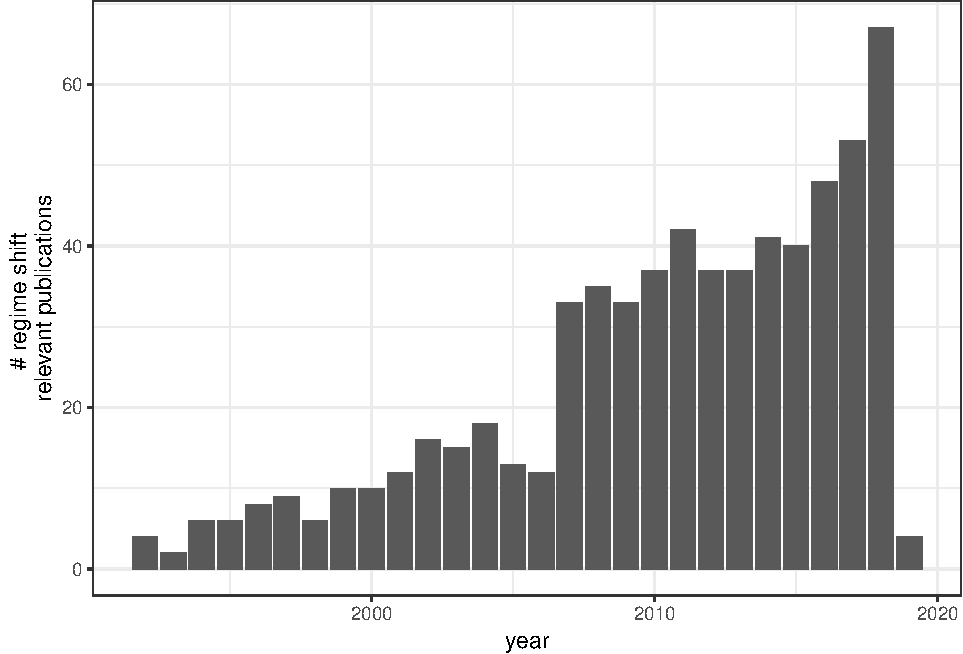
\includegraphics{_myDissertation_files/figure-latex/wosRegimePubsByYear-1.pdf}
\caption{\label{fig:wosRegimePubsByYear}Number of publications by year in
fields `Ecology' and `Biodiversity Conservation' which included terms
related to `regime shift' (total = 654).}
\end{figure}
\section{Results}\label{results}
\begin{Shaded}
\begin{Highlighting}[]
 \KeywordTok{ggplot}\NormalTok{(wos.regime.plotData }\OperatorTok
\StringTok{              }\KeywordTok{group_by}\NormalTok{(journal) }\OperatorTok\StringTok{ }
\StringTok{              }\KeywordTok{summarise}\NormalTok{(}\DataTypeTok{nJrnl =} \KeywordTok{n}\NormalTok{()) }\OperatorTok\StringTok{ }
\StringTok{               }\KeywordTok{filter}\NormalTok{(nJrnl }\OperatorTok{>=}\StringTok{ }\DecValTok{10}\NormalTok{, }
\NormalTok{                      journal }\OperatorTok{!=}\StringTok{ "NA"}\NormalTok{) }\OperatorTok\StringTok{ }
\StringTok{               }\KeywordTok{arrange}\NormalTok{(nJrnl)) }\OperatorTok{+}
\StringTok{  }\KeywordTok{geom_bar}\NormalTok{(}\KeywordTok{aes}\NormalTok{(}\DataTypeTok{x =}\NormalTok{  journal, }\DataTypeTok{y =}\NormalTok{ nJrnl), }\DataTypeTok{stat=} \StringTok{"identity"}\NormalTok{)}\OperatorTok{+}
\StringTok{  }\KeywordTok{ylab}\NormalTok{(}\StringTok{'number of articles'}\NormalTok{) }\OperatorTok{+}\StringTok{ }\KeywordTok{xlab}\NormalTok{(}\StringTok{""}\NormalTok{) }\OperatorTok{+}
\StringTok{  }\KeywordTok{coord_flip}\NormalTok{()}\OperatorTok{+}
\StringTok{  }\KeywordTok{theme_bw}\NormalTok{() }\OperatorTok{+}\StringTok{ }
\StringTok{  }\KeywordTok{theme}\NormalTok{(}\DataTypeTok{axis.text.y =} \KeywordTok{element_text}\NormalTok{( }\DataTypeTok{hjust =} \DecValTok{1}\NormalTok{, }\DataTypeTok{size =} \DecValTok{4}\NormalTok{))}\OperatorTok{+}
\StringTok{  }\KeywordTok{theme}\NormalTok{(}\DataTypeTok{axis.title.x =} \KeywordTok{element_text}\NormalTok{(}\DataTypeTok{size =} \DecValTok{8}\NormalTok{))}
\end{Highlighting}
\end{Shaded}
\begin{figure}
\centering
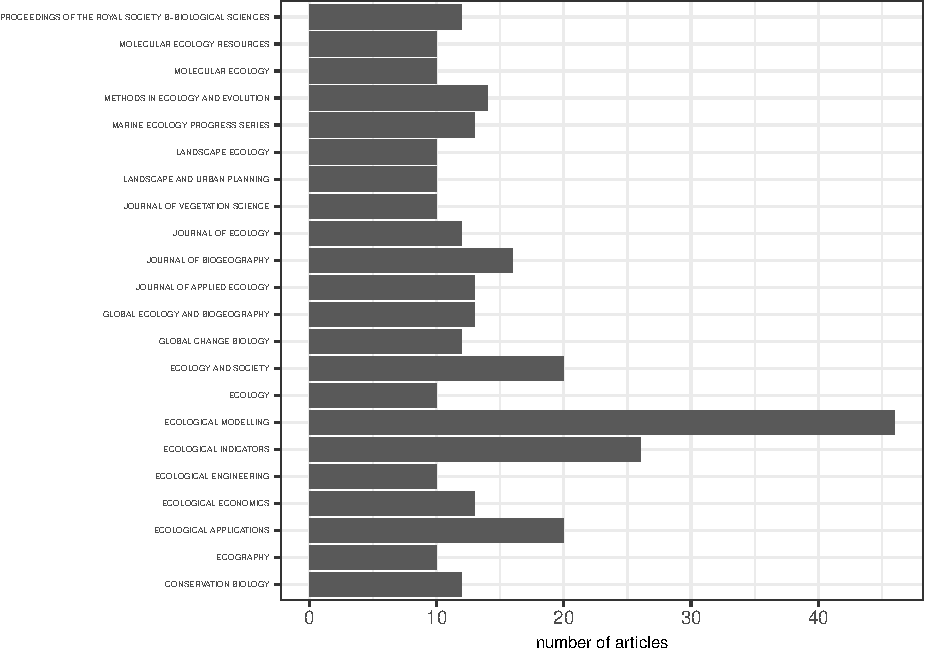
\includegraphics{_myDissertation_files/figure-latex/wosRegimePubsByJrnlmin10Pubs-1.pdf}
\caption{\label{fig:wosRegimePubsByJrnlmin10Pubs}Distribution of the `regime
shift' articles for journals with at least 10 articles.}
\end{figure}
\subsection{Web of Science}\label{web-of-science-1}

The search boolean for WoS boolean \emph{not} including restriction to
fields (WC) `Ecology' and `Conservation Biology' yielded over 20,000
results. Restricting to the abovementioned fields created a manageable
database from which to filter. This search yielded 2,776 articles. 654
of these papers included terms relating to `regime shifts' (Figure
\ref{fig:wosRegimePubsByYear}), many appearing in the journal
\emph{Ecological Modelling} (Figure
\ref{fig:wosRegimePubsByJrnlmin10Pubs}). The rate of publication of
`regime shift' articles is not strongly correlated with the rate of
papers published in `Ecology' and `Biodiversity Conservation' fields
(Figure \ref{fig:wosRegimePubsByYearwithNumEcolPubs}).
\begin{Shaded}
\begin{Highlighting}[]
\KeywordTok{ggplot}\NormalTok{(wos.regime.plotData }\OperatorTok\StringTok{ }
\StringTok{               }\KeywordTok{distinct}\NormalTok{(year, }\DataTypeTok{.keep_all=}\NormalTok{T)) }\OperatorTok{+}
\StringTok{    }\KeywordTok{geom_bar}\NormalTok{(}\KeywordTok{aes}\NormalTok{(}\DataTypeTok{x =}\NormalTok{ year, }\DataTypeTok{y =}\NormalTok{ nRegime.pubs, }\DataTypeTok{color =} \StringTok{"Regime shift"}\NormalTok{), }\DataTypeTok{stat=} \StringTok{"identity"}\NormalTok{ )}\OperatorTok{+}\StringTok{ }
\StringTok{  }\KeywordTok{geom_line}\NormalTok{(wos.all.ecol, }\DataTypeTok{mapping =} \KeywordTok{aes}\NormalTok{(}\DataTypeTok{x =}\NormalTok{ year, }\DataTypeTok{y =}\NormalTok{ nEcol.pubs}\OperatorTok{/}\FloatTok{1e3}\NormalTok{, }\DataTypeTok{color =} \StringTok{"All ecology"}\NormalTok{), }\DataTypeTok{size =} \FloatTok{1.3}\NormalTok{)}\OperatorTok{+}
\StringTok{  }\KeywordTok{scale_y_continuous}\NormalTok{(}\DataTypeTok{sec.axis =} \KeywordTok{sec_axis}\NormalTok{(}\OperatorTok{~}\NormalTok{.}\OperatorTok{*}\DecValTok{1000}\NormalTok{, }\DataTypeTok{name =} \StringTok{"# all ecology publications}\CharTok{\textbackslash{}n}\StringTok{ (line)"}\NormalTok{)) }\OperatorTok{+}\StringTok{ }
\StringTok{  }\KeywordTok{scale_colour_manual}\NormalTok{(}\DataTypeTok{values =} \KeywordTok{c}\NormalTok{(}\StringTok{"red"}\NormalTok{, }\StringTok{"black"}\NormalTok{ )) }\OperatorTok{+}
\StringTok{  }\KeywordTok{labs}\NormalTok{(}\DataTypeTok{y =} \StringTok{"# regime shift }\CharTok{\textbackslash{}n}\StringTok{ relevant publications "}\NormalTok{,}
              \DataTypeTok{x =} \StringTok{"year"}\NormalTok{,}
              \DataTypeTok{colour =} \StringTok{"Publication type"}\NormalTok{)}\OperatorTok{+}\StringTok{ }
\StringTok{  }\KeywordTok{theme}\NormalTok{(}\DataTypeTok{legend.position =} \KeywordTok{c}\NormalTok{(}\DecValTok{1998}\NormalTok{,}\DecValTok{60000}\NormalTok{), }\DataTypeTok{axis.title.y =} \KeywordTok{element_text}\NormalTok{(}\DataTypeTok{size =} \DecValTok{10}\NormalTok{))}
\end{Highlighting}
\end{Shaded}
\begin{figure}
\centering
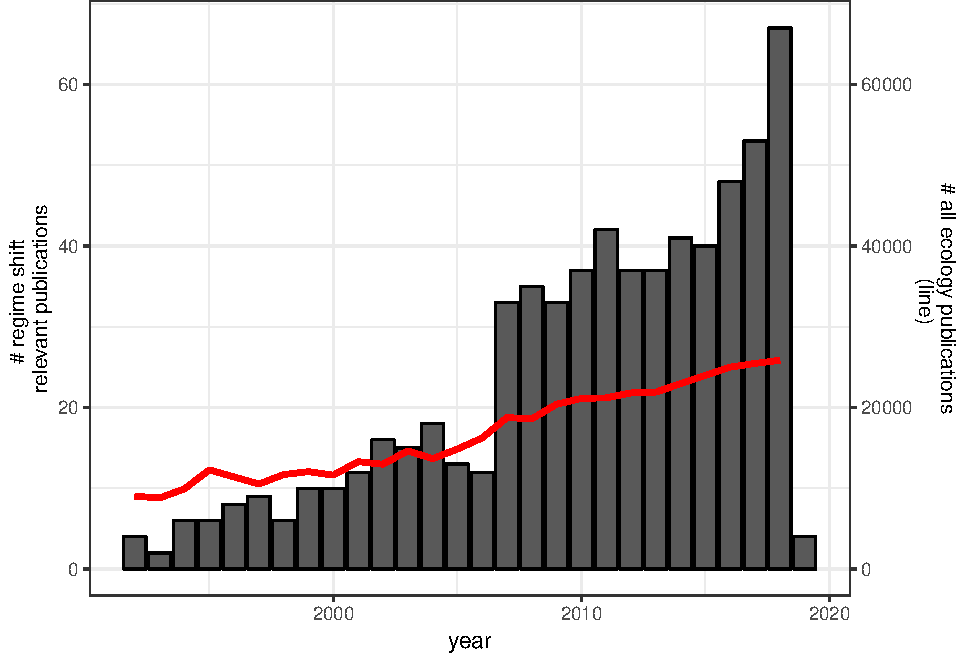
\includegraphics{_myDissertation_files/figure-latex/wosRegimePubsByYearwithNumEcolPubs-1.pdf}
\caption{\label{fig:wosRegimePubsByYearwithNumEcolPubs}Number of
publications by year in fields `Ecology' and `Biodiversity Conservation'
which included terms related to `regime shift' (total = 654).}
\end{figure}
Filtering this WoS results to include only articles mentioning terms
related to `new method' yielded 202 articles. After removing prior
knowledge, only 93 articles remained to be reviewed `by hand' (i.e.,
reading the entire paper). Only 2 `new' methods were identified from the
WoS search (\ref{fig:rdmReviewFlow}).

\subsection{Google Scholar and prior
knowledge}\label{google-scholar-and-prior-knowledge}

Of the 250 articles scanned in Google Scholar, I retained 3 methods. I
was previously aware of an additional 68 articles containing `new'
methods (\ref{fig:rdmReviewFlow}).
\begin{Shaded}
\begin{Highlighting}[]
\NormalTok{webshot}\OperatorTok{::}\KeywordTok{install_phantomjs}\NormalTok{()}
\end{Highlighting}
\end{Shaded}
\begin{verbatim}
phantomjs has been installed to /Users/jessicaburnett/Library/Application Support/PhantomJS
\end{verbatim}
\begin{Shaded}
\begin{Highlighting}[]
\NormalTok{DiagrammeR}\OperatorTok{::}\KeywordTok{grViz}\NormalTok{(}
  \StringTok{"digraph \{}
\StringTok{  graph [layout = dot, rankdir = TB]}

\StringTok{  # define the global styles of the nodes. We can override these in box if we wish}
\StringTok{  node [shape = rectangle, style = filled, fillcolor = White, fixedsize = TRUE, width=2, height=1]}
\StringTok{  data0 [label = 'Web of Science }\CharTok{\textbackslash{}n}\StringTok{ initial search }\CharTok{\textbackslash{}n}\StringTok{ (n = 2,776)', shape = folder, fillcolor = Linen]}
\StringTok{  data1 [label = 'Filtering }\CharTok{\textbackslash{}n}\StringTok{ by title & abstract }\CharTok{\textbackslash{}n}\StringTok{ (n = 202)', ]}
\StringTok{  data2 [label = 'Filter by }\CharTok{\textbackslash{}n}\StringTok{ prior knowledge }\CharTok{\textbackslash{}n}\StringTok{ (n = 93)']}
\StringTok{  data3 [label = 'Filtered by hand }\CharTok{\textbackslash{}n}\StringTok{ (n = 2)']}
\StringTok{  }
\StringTok{  gs1 [label = 'Informal Google }\CharTok{\textbackslash{}n}\StringTok{ Scholar search }\CharTok{\textbackslash{}n}\StringTok{ (n = 250)', shape = folder, fillcolor = Linen]}
\StringTok{  gs2 [label = 'Filtering by hand }\CharTok{\textbackslash{}n}\StringTok{ (n = 3)', shape = circle]}

\StringTok{   }
\StringTok{  prior [label = 'Prior knowledge }\CharTok{\textbackslash{}n}\StringTok{ (n = 68)', shape = circle, fillcolor = Linen]}
\StringTok{  data4 [label = 'Priors + }\CharTok{\textbackslash{}n}\StringTok{ Google Scholar }\CharTok{\textbackslash{}n}\StringTok{ (n = 71)', shape = circle]}
\StringTok{  }
\StringTok{  results [label = 'Final list of }\CharTok{\textbackslash{}n}\StringTok{ methods }\CharTok{\textbackslash{}n}\StringTok{ (n = 73)', shape = circle, fillcolor = Red]}

\StringTok{# edge definitions with the node IDs}
\StringTok{data0 -> data1 ->data2 ->data3 ->results}
\StringTok{gs1 -> gs2 -> data4 -> results}
\StringTok{prior -> data4}

\StringTok{\}"}
\NormalTok{  )}
\end{Highlighting}
\end{Shaded}
\begin{figure}
\centering
\includegraphics{_myDissertation_files/figure-latex/rdmReviewFlow-1.pdf}
\caption{\label{fig:rdmReviewFlow}Flowchart of the litearture review process
for identifying new regime detection methods. *Only the first ten pages
(250 articles) of Google Scholar results were examined. Node shapes:
folder = unfiltered articles; box = articles actively filtered; diamond
= number of articles with new methods.}
\end{figure}
\subsection{List of new methods}\label{list-of-new-methods}
\begin{Shaded}
\begin{Highlighting}[]
\KeywordTok{require}\NormalTok{(kableExtra, }\DataTypeTok{quietly =}\NormalTok{ T)}
\end{Highlighting}
\end{Shaded}
\begin{verbatim}

Attaching package: 'kableExtra'
\end{verbatim}
\begin{verbatim}
The following object is masked from 'package:dplyr':

    group_rows
\end{verbatim}
\begin{Shaded}
\begin{Highlighting}[]
\NormalTok{long_dt <-}\StringTok{ }\NormalTok{finalMetricsList  }\OperatorTok
\StringTok{  }\KeywordTok{mutate}\NormalTok{(}\DataTypeTok{label2 =} \KeywordTok{paste0}\NormalTok{(}\StringTok{"@"}\NormalTok{,myLabel1)) }\OperatorTok
\StringTok{  }\NormalTok{dplyr}\OperatorTok{::}\KeywordTok{select}\NormalTok{(method, type1,label2 )}

\KeywordTok{kable}\NormalTok{(long_dt, }\StringTok{"latex"}\NormalTok{, }\DataTypeTok{longtable =}\NormalTok{ T, }\DataTypeTok{booktabs =}\NormalTok{ T,   }\DataTypeTok{caption =} \StringTok{"Longtable"}\NormalTok{) }\OperatorTok
\CommentTok{# add_header_above(c(" ", "Group 1" = 5, "Group 2" = 6)) %>%}
\StringTok{  }\KeywordTok{kable_styling}\NormalTok{(}\DataTypeTok{latex_options =} \KeywordTok{c}\NormalTok{(}\StringTok{"repeat_header"}\NormalTok{))}
\end{Highlighting}
\end{Shaded}
\begin{longtable}{lll}
\caption{\label{tab:methodsMetricsListTab}Longtable}\\
\toprule
method & type1 & label2\\
\midrule
\endfirsthead
\caption[]{\label{tab:methodsMetricsListTab}Longtable \textit{(continued)}}\\
\toprule
method & type1 & label2\\
\midrule
\endhead
\
\endfoot
\bottomrule
\endlastfoot
Autocorrelation at-lag-1 & metric & @vincent1998technique\\
Autoregressive coefficient of AR(1) & metric & @held2004detection\\
Inverse of AR(1) coefficient & metric & @carpenter2008leading\\
Detrended fluctuation analysis & metric & @livina2007modified\\
Spectral density & metric & @kleinen2003potential\\
\addlinespace
Spectral ratio & metric & @biggs2009turning\\
Spectral exponent & metric & @andersen\_ecological\_2009\\
Standard deviation & metric & @carpenter2006rising\\
Coefficient of variation (CV) & metric & @carpenter2006rising\\
Skewness & metric & @guttal2008changing\\
\addlinespace
Kurtosis & metric & @biggs2009turning\\
Conditional heteroskedasticity & metric & @seekell2011conditional\\
BDS test & metric & @carpenterBrock2011early\\
Time-varying AR(p) model & model & @ives2012detecting\\
Nonparametric drift-diffusion-jump model & model & @carpenter2011early\\
\addlinespace
Potential analysis & model & @ives2012detecting\\
Fourier Analysis & NA & @carpenter2010early\\
T-test & metric & @ducre2003comparison\\
Bayesian approaches & model & @jo2016bayesian\\
Mann-whitney U-test & metric & @mauget2003multidecadal\\
\addlinespace
Wilcoxon rank-sum & metric & @karl1987approach\\
Pettitt test & metric & @pettitt1979non\\
Mann-Kendall test & metric & @goossens1987recognize\\
LePage test & metric & @yonetani1993detection\\
Standard normal homoegeneity & metric & @alexandersson1986homogeneity\\
\addlinespace
Regression-based models & model & @solow1987testing\\
Oerleman's method & metric & @oerlemans1978objective\\
Cumulative deviation test (CUSUM) & metric & @buishand1982some\\
Signal-to-noise ratio & metric & @NA\\
Intervention Analysis & metric & @francis1994decadal\\
\addlinespace
STARS & metric & @buishand1982some\\
MCMC & NA & @NA\\
Quickest detection method (Shiryaev<d0>Roberts statistic) & metric & @moustakides2009numerical\\
Variance Index & metric & @brock\_variance\_2006\\
Spectrum indicator & metric & @NA\\
\addlinespace
Wavelet analysis (decomposition) & NA & @cazelles2008wavelet\\
Downton-Katz test & metric & @karl1987approach\\
Rodionov method & metric & @rodionov\_sequential\_2005\\
Nikiforiv method & metric & @NA\\
Average standard deviates & metric & @ebbesmeyer19911976\\
\addlinespace
Fisher Information & metric & @fath\_regime\_2003\\
Vector-autoregressive method & NA & @solow\_test\_2005\\
Lanzante method & NA & @lanzante1996resistant\\
Free-knot splines \& piecewise linear modelling & NA & @gal2010novel\\
Self-exciting threshold autoregressive state-space model SETARSS(p) & model & @tong1990nonlinear\\
\addlinespace
Smooth transition autoregressive model & model & @see gal2010novel\\
Moving detrended fluctuation analysis (MDFA) & metric & @he2008new\\
Nearest-neighbor statistics & metric & @pawlowski\_identification\_2008\\
Clustering, various & NA & @NA\\
dimension reduction techniques (e.g., PCA) & metric & @NA\\
\addlinespace
Sequential tests/moving windows & metric & @NA\\
Online dynamic linear modelling +  time\_varying autoregressive state\_space models (TVARSS) & models & @parparov2017quantifying\\
Stability Index of the Ecological Units & metric & @parparov2015quantifying\\
Generalized model & model & @lade2012early\\
Threshold Indicator Taxa ANalysis (TITAN) & metric & @baker2010new\\
\addlinespace
Convex model & model & @qi2016resilience\\
Probability density function entropy method & metric & @pawlowski\_identification\_2008\\
Method 1-TBD & NA & @manly2006two\\
method-fuzzy synthetic evaluation (FSE) & NA & @wang2011application\\
Method 2-TBD & NA & @manly2006two\\
\addlinespace
Zonal thresholding & metric* & @yin2017methods\\
Characteristic length scale (CLS) estimation & attractor reconstruction & @NA\\
two-phase regression & metric of a model & @easterling1995new\\
shiftogram & model & @groger2011analyses\\*
\end{longtable}
Using my prior knowledge of the relevant litearture, referring to
previous review articles, and searching both Web of Science and Google
Scholar, I identified 64 unique RDMs (Figure \ref{fig:rdmReviewFlow};
Table \ref{methodsMetricsListTab}).
\begin{Shaded}
\begin{Highlighting}[]
\NormalTok{yearTemp <-}\StringTok{ }\NormalTok{finalMetricsList.bib }\OperatorTok\StringTok{ }
\StringTok{  }\KeywordTok{group_by}\NormalTok{(year) }\OperatorTok\StringTok{ }
\StringTok{  }\KeywordTok{summarise}\NormalTok{(}\DataTypeTok{n =} \KeywordTok{n}\NormalTok{()) }

\KeywordTok{ggplot}\NormalTok{(yearTemp ) }\OperatorTok{+}
\StringTok{  }\KeywordTok{geom_bar}\NormalTok{(}\KeywordTok{aes}\NormalTok{(}\DataTypeTok{x =}\NormalTok{ year, }\DataTypeTok{y =}\NormalTok{n), }\DataTypeTok{stat =} \StringTok{'identity'}\NormalTok{) }\OperatorTok{+}
\StringTok{  }\KeywordTok{ylab}\NormalTok{(}\StringTok{"articles published "}\NormalTok{) }\OperatorTok{+}\StringTok{ }\KeywordTok{xlab}\NormalTok{(}\StringTok{'publication year'}\NormalTok{) }\OperatorTok{+}
\StringTok{  }\KeywordTok{theme_bw}\NormalTok{() }\OperatorTok{+}\StringTok{ }\KeywordTok{theme}\NormalTok{(}\DataTypeTok{axis.text.x =} \KeywordTok{element_text}\NormalTok{(}\DataTypeTok{angle =} \DecValTok{90}\NormalTok{, }\DataTypeTok{hjust =} \DecValTok{1}\NormalTok{, }\DataTypeTok{size =} \DecValTok{12}\NormalTok{))}
\end{Highlighting}
\end{Shaded}
\begin{figure}
\centering
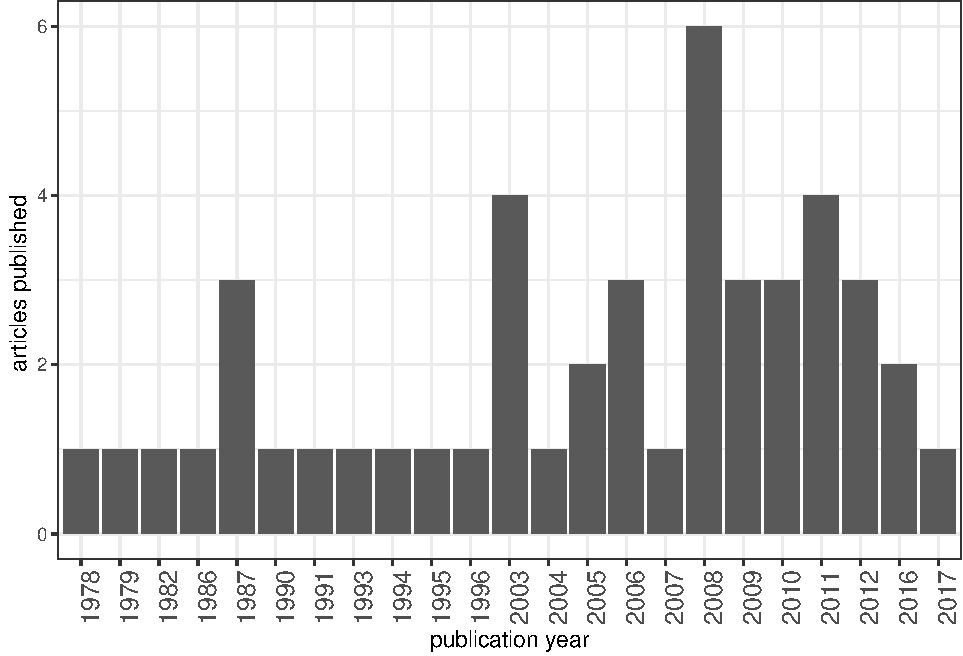
\includegraphics{_myDissertation_files/figure-latex/jrnlYearFig-1.pdf}
\caption{\label{fig:jrnlYearFig}Number of methods publisheed over time.}
\end{figure}
\section{Discussion}\label{discussion}

In this chapter I highlighted the plethora of regime detection metrics
(RDMs) proposed in the literature for analyzing ecological data (Table
\ref{methodsMetricsListTab}). Although multiple reviews of RDMs exist,
they are not comprehensive in their survey of the possible methods. Most
reviews have summarized various aspects of RDMs. For example, Roberts et
al. (2018) summarizes methods capable of handling multiple (c.f. a
single) variable, and Dakos et al. (2015b) review only methods designed
to detect the phenomenon of critical slowing down. Here, I did not
discriminate--rather, I present an exaustive list of the plethora of
methods proposed for detecting ecological detect regime shifts,
\emph{sensu lato}, providing a much-needed update to collection provided
by S. N. Rodionov (2005), and other review papers (Mac Nally et al.,
2014, Scheffer et al. (2015), S. N. Rodionov (2005), Roberts et al.
(2018), Dakos et al. (2015b), Mantua (2004), Litzow \& Hunsicker (2016),
Kefi et al. (2014), Andersen et al. (2009), Boettiger et al. (2013),
Dakos et al. (2015a), Clements \& Ozgul (2018), Filatova et al. (2016),
deYoung et al. (2008)).

\subsection{Barriers to identifying new
RDMs}\label{barriers-to-identifying-new-rdms}

Clearly, as was shown in this chapter (Figure \ref{fig:rdmReviewFlow}),
a systematic review of the ecological literature will likely not yield
anywhere near a comprehensive list of the RDMs proposed and/or used.
This disaparity may be due to both my search methods and to the current
state of regime shift research in ecology.

First, my review restricted articles to articles suggesting they were
introducing a `new method' as n RDM. Avoiding this potential barrier
would have required I review the titles, abstracts, and bodies of over
22,000 articles (Figure \ref{fig:rdmReviewFlow}). Alternatively, this
may also be ameliorated by searching the relevant literature for
\emph{applications} of RDMs to ecological data, however, I suspect this
would similarly yield a large number of articles to review.

Next, only a handful of methods have been introduced to the mainstream
methodological journals in ecology (e.g., \emph{Ecological Modelling},
\emph{Methods in Ecology and Evolution}; Figure \ref{fig:jrnlDistFig}).
Although many mainstream publications (e.g., \emph{Science},
\emph{Ecology Letters}) include applications of some of the methods
identified in this chapter (Table \ref{methodsMetricsListTab}), I argue
that celebrity and `new and shiny' (Steel, Kennedy, Cunningham, \&
Stanovick, 2013) methods may influence which methodological articles are
printed in these popular journals.
\begin{Shaded}
\begin{Highlighting}[]
\CommentTok{# Visualize results}
\NormalTok{jrnlTemp <-}\StringTok{ }\NormalTok{finalMetricsList.bib }\OperatorTok\StringTok{ }
\StringTok{  }\KeywordTok{mutate}\NormalTok{(}\DataTypeTok{journal =} \KeywordTok{ifelse}\NormalTok{(label }\OperatorTok{==}\StringTok{"rodionov_sequential_2005"}\NormalTok{, }\StringTok{"Other"}\NormalTok{, journal), }
         \DataTypeTok{journal =} \KeywordTok{ifelse}\NormalTok{(label }\OperatorTok{==}\StringTok{"tong1990nonlinear"}\NormalTok{, }\StringTok{"Other"}\NormalTok{, journal), }
         \DataTypeTok{journal =} \KeywordTok{ifelse}\NormalTok{(journal }\OperatorTok{==}\StringTok{"International Journal of Climatology: A Journal of the Royal Meteorological Society"}\NormalTok{, }\StringTok{"International Journal of Climatology"}\NormalTok{, journal), }
         \DataTypeTok{journal =} \KeywordTok{ifelse}\NormalTok{(journal }\OperatorTok\StringTok{ }\KeywordTok{c}\NormalTok{(}\OtherTok{NA}\NormalTok{, }\StringTok{"NA"}\NormalTok{), }\StringTok{"Other"}\NormalTok{, journal)) }\OperatorTok\StringTok{ }
\StringTok{  }\KeywordTok{mutate}\NormalTok{(}\DataTypeTok{journal =} \KeywordTok{toupper}\NormalTok{(journal)) }\OperatorTok\StringTok{ }
\StringTok{  }\KeywordTok{group_by}\NormalTok{(journal) }\OperatorTok\StringTok{ }
\StringTok{  }\KeywordTok{summarise}\NormalTok{(}\DataTypeTok{n =} \KeywordTok{n}\NormalTok{()) }

\NormalTok{ggplot2}\OperatorTok{::}\KeywordTok{ggplot}\NormalTok{(jrnlTemp) }\OperatorTok{+}
\StringTok{  }\KeywordTok{geom_bar}\NormalTok{(}\KeywordTok{aes}\NormalTok{(}\DataTypeTok{x =}\NormalTok{ journal, }\DataTypeTok{y =}\NormalTok{n), }\DataTypeTok{stat =} \StringTok{'identity'}\NormalTok{) }\OperatorTok{+}
\StringTok{  }\KeywordTok{ylab}\NormalTok{(}\StringTok{'number of articles'}\NormalTok{) }\OperatorTok{+}\StringTok{ }\KeywordTok{xlab}\NormalTok{(}\StringTok{""}\NormalTok{) }\OperatorTok{+}
\StringTok{  }\KeywordTok{coord_flip}\NormalTok{()}\OperatorTok{+}
\StringTok{  }\KeywordTok{theme_bw}\NormalTok{() }\OperatorTok{+}\StringTok{ }
\StringTok{  }\KeywordTok{theme}\NormalTok{(}\DataTypeTok{axis.text.y =} \KeywordTok{element_text}\NormalTok{( }\DataTypeTok{hjust =} \DecValTok{1}\NormalTok{, }\DataTypeTok{size =} \DecValTok{8}\NormalTok{))}
\end{Highlighting}
\end{Shaded}
\begin{figure}
\centering
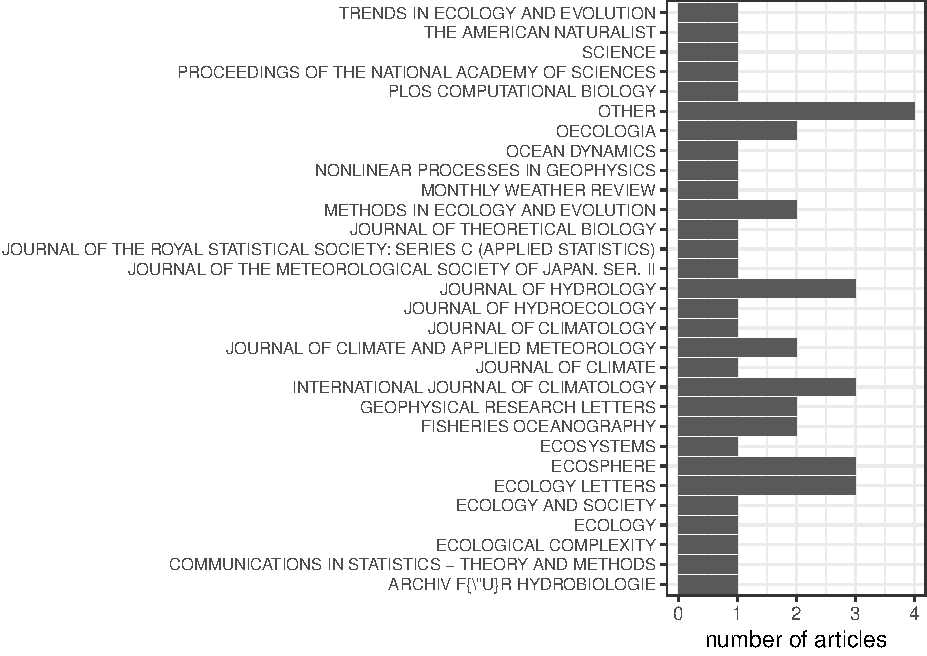
\includegraphics{_myDissertation_files/figure-latex/jrnlDistFig-1.pdf}
\caption{\label{fig:jrnlDistFig}Distribution of identified methods across
publications. Note: books, reports, and articles without original
reference coded as `Other'}
\end{figure}
A critical survey of potetial and realized applications of these methods
would be useful for highlighting the needs of future research and
methodological improvements. Many of the methods presented in Table
\ref{methodsMetricsListTab} have either not been applied to empirical
data at all, or were tested only once (often but not always in the
article introducing the method). Some methods, especially those dubbed
`early warning indicators' (variance, autoregressive model coefficients)
have become relativley mainstream in their application to empirical
data, however, have been shown to be less robust to noisy and nonlinear
systems data (Burthe et al., 2016) and systems not exhibiting
catstrophic shifts (Dutta, Sharma, \& Abbott, 2018). Most other methods
have yet to be rigorously tested on noisy, high dimensional, empirical
data. Further, the methods which are not mainstream but have been
applied to one of these data types have not any statistical indicators
associated with confirming the existence and location of the regime
shift.

As shown this chapter, identifying RDMs using traditional literature
review techniques may prove difficult. Many of the methods identified in
my review were not identified using Web of Science or Google
Scholar--rather, I was either previously aware of most of the methods,
and many others were highlighted in previous RDM reviews {]}. To
facilitate this process, an online, comprehensive database may prove
useful to the practical ecologist.

\subsection{Conclusions}\label{conclusions}

To make the regime detection methods (RDMs) more available and
transparent to the practical ecologist, I recommend the following: 1.
consitent use of fewer methods 1. persistent collection and maintenance
of baseline data (reference data) 1. an on-line database of all RDMs -
open-sourced - linked to the original sources (in ecology and statistics
or mathematics) - linked to applications 1. a critical review of the
current state of RDMs in ecology - including methodological advancements
- especially highlighting where the method fails to perform - including
historical tracking of specific methods to identify which may need to be
retired, rather than resuscitated 1. more empirical applications of
these methods (especially of those only tested on toy and experimental
data) 1. relation of RDMs in ecology to other fields (computer science,
data science, climatology and oceanography)

I suggest below a suite of questions which may provide useful in a
critical review of the characteristics, rigor, and promise of RDMs in
the context of ecological data analysis.
\begin{Shaded}
\begin{Highlighting}[]
\NormalTok{Questions.stat <-}\StringTok{ }\KeywordTok{c}\NormalTok{(}
  \StringTok{"What are the major assumptions about the distribution?"}\NormalTok{,}
  \StringTok{"Does the method explicitly assume stationarity? If not, can it handle non-stationary processes?"}\NormalTok{, }
  \StringTok{"Does the performance of the method change with non-stationarity?"}\NormalTok{,}
  \StringTok{"Can the method handle unstructured data (information)?"}\NormalTok{,}
  \StringTok{"Does the regime shift need to be identified *a priori*?"}\NormalTok{,}
  \StringTok{"Can the method handle multiple regime shifts?"}\NormalTok{,}
  \StringTok{"Does the performance of the method change with non-stationarity?"}\NormalTok{,}
  \StringTok{"What types of regime shifts can the method detect (e.g., stochastic resonance, slow-fast cycles, noise-induced transition)?"}\NormalTok{,}
  \StringTok{"Is it a model- or metric-based method?"}\NormalTok{, }
  \StringTok{"Does it have forecasting potential?"}\NormalTok{,}
  \StringTok{"Can the method handle uneven sampling?"}\NormalTok{,}
  \StringTok{"What are the minimum data requirements (resolution, extent, number of observations)?"}\NormalTok{,}
  \StringTok{"How does the method handle missing data (e.g., new invasions)?"}\NormalTok{, }
  \StringTok{"Does the method assume Eulerian or Lagrangian processes?"}\NormalTok{)}

\NormalTok{Questions.ecol <-}\StringTok{ }\KeywordTok{c}\NormalTok{(}
  \StringTok{"Has the method been tested on empirical data? If so, to what rigor?"}\NormalTok{,}
  \StringTok{"What is the impact of losing state variables on long-term predictions (e.g., species extinction)?"}\NormalTok{,}
  \StringTok{"Can the method identify drivers?"}\NormalTok{,}
  \StringTok{"What assumptions does the method make about the system?"}\NormalTok{, }
  \StringTok{"What types of regime shifts are possible in the system?"}\NormalTok{, }
  \StringTok{"Are regime shift(s) suspected *a priori*?"}\NormalTok{,}
  \StringTok{"What lag(s) exist in the data (system)?"}\NormalTok{,}
  \StringTok{"Would a positive forecast change management action?"}\NormalTok{,}
  \StringTok{"Do predictions translate to other systems?"}\NormalTok{,}
  \StringTok{"Can we interpolate data if necessary? If so, what does this mean for inference?"}\NormalTok{,}
  \StringTok{"In which discipline(s) beyond ecology has the method been tested?"}
\NormalTok{  )}

\NormalTok{Questions =}\StringTok{ }\KeywordTok{tibble}\NormalTok{(}\DataTypeTok{Type =} \KeywordTok{c}\NormalTok{(}\StringTok{"Methodological"}\NormalTok{, }\KeywordTok{rep}\NormalTok{(}\StringTok{""}\NormalTok{, }\KeywordTok{length}\NormalTok{(Questions.stat)}\OperatorTok{-}\DecValTok{1}\NormalTok{),}\StringTok{"Ecological"}\NormalTok{  , }\KeywordTok{rep}\NormalTok{(}\StringTok{""}\NormalTok{, }\KeywordTok{length}\NormalTok{(Questions.ecol)}\OperatorTok{-}\DecValTok{1}\NormalTok{)), }
                       \DataTypeTok{Questions =} \KeywordTok{c}\NormalTok{(Questions.stat, Questions.ecol))}
\KeywordTok{require}\NormalTok{(kableExtra, }\DataTypeTok{quietly =}\NormalTok{ T)}
\KeywordTok{kable}\NormalTok{(Questions, }\StringTok{"latex"}\NormalTok{, }\DataTypeTok{longtable =}\NormalTok{ T, }\DataTypeTok{booktabs =}\NormalTok{ T,   }\DataTypeTok{caption =} \StringTok{"Potential questions for a comprehensive review of the ecological regime detection metrics literature."}\NormalTok{) }\OperatorTok
\StringTok{ }\KeywordTok{kable_styling}\NormalTok{(}\DataTypeTok{full_width =}\NormalTok{ F) }\OperatorTok
\StringTok{ }\KeywordTok{column_spec}\NormalTok{(}\DecValTok{1}\NormalTok{, }\DataTypeTok{bold =}\NormalTok{ T, }\DataTypeTok{border_right =}\NormalTok{ T) }\OperatorTok
\StringTok{  }\CommentTok{# CANNOT figure out how to use COLLAPSE AND column_spec width at the same time........}
\StringTok{ }\CommentTok{# collapse_rows(columns = 1, valign = "middle", latex_hline = "major") %>%}
\StringTok{ }\KeywordTok{column_spec}\NormalTok{(}\DecValTok{2}\NormalTok{, }\DataTypeTok{bold =}\NormalTok{ F, }\DataTypeTok{width =} \StringTok{"30em"}\NormalTok{)}
\end{Highlighting}
\end{Shaded}
\begin{longtable}{>{\bfseries}l|>{\raggedright\arraybackslash}p{30em}}
\caption{\label{tab:nextStepsTab}Potential questions for a comprehensive review of the ecological regime detection metrics literature.}\\
\toprule
Type & Questions\\
\midrule
Methodological & What are the major assumptions about the distribution?\\
 & Does the method explicitly assume stationarity? If not, can it handle non-stationary processes?\\
 & Does the performance of the method change with non-stationarity?\\
 & Can the method handle unstructured data (information)?\\
 & Does the regime shift need to be identified *a priori*?\\
\addlinespace
 & Can the method handle multiple regime shifts?\\
 & Does the performance of the method change with non-stationarity?\\
 & What types of regime shifts can the method detect (e.g., stochastic resonance, slow-fast cycles, noise-induced transition)?\\
 & Is it a model- or metric-based method?\\
 & Does it have forecasting potential?\\
\addlinespace
 & Can the method handle uneven sampling?\\
 & What are the minimum data requirements (resolution, extent, number of observations)?\\
 & How does the method handle missing data (e.g., new invasions)?\\
 & Does the method assume Eulerian or Lagrangian processes?\\
Ecological & Has the method been tested on empirical data? If so, to what rigor?\\
\addlinespace
 & What is the impact of losing state variables on long-term predictions (e.g., species extinction)?\\
 & Can the method identify drivers?\\
 & What assumptions does the method make about the system?\\
 & What types of regime shifts are possible in the system?\\
 & Are regime shift(s) suspected *a priori*?\\
\addlinespace
 & What lag(s) exist in the data (system)?\\
 & Would a positive forecast change management action?\\
 & Do predictions translate to other systems?\\
 & Can we interpolate data if necessary? If so, what does this mean for inference?\\
 & In which discipline(s) beyond ecology has the method been tested?\\
\bottomrule
\end{longtable}
\chapter{A guide to Fisher Information for Ecologists}\label{fiGuide}

\emph{This chapter is intended for submission to the publication
\emph{Methods in Ecology and Evolution}.\footnote{Co-authors include:
  N.B. Price, A.J. Tyre, C.R. Allen, T. Eason, D.G. Angeler, and D.
  Twidwell}}
\begin{Shaded}
\begin{Highlighting}[]
\CommentTok{# Model parameters}
\NormalTok{parameters <-}\StringTok{ }\KeywordTok{c}\NormalTok{(}
  \DataTypeTok{g1 =} \DecValTok{1}\NormalTok{,}
  \DataTypeTok{m2 =} \DecValTok{1}\NormalTok{,}
  \DataTypeTok{l12 =} \FloatTok{0.01}\NormalTok{,}
  \DataTypeTok{g21 =} \FloatTok{0.01}\NormalTok{,}
  \DataTypeTok{k =} \DecValTok{625}\NormalTok{,}
  \DataTypeTok{B =} \FloatTok{0.005}
\NormalTok{)}

\CommentTok{# Initial conditions}
\NormalTok{state <-}\StringTok{ }\KeywordTok{c}\NormalTok{(}
  \DataTypeTok{x1 =} \FloatTok{277.7815}\NormalTok{, }
  \DataTypeTok{x2 =} \FloatTok{174.551}
\NormalTok{)}

\CommentTok{# System differential equations (eq. 7.17 and 7.18)}
\NormalTok{deq <-}\StringTok{ }\ControlFlowTok{function}\NormalTok{(t, state, parameters) \{}
  \KeywordTok{with}\NormalTok{(}\KeywordTok{as.list}\NormalTok{(}\KeywordTok{c}\NormalTok{(state, parameters)), \{}
\NormalTok{    dx1dt <-}\StringTok{ }\NormalTok{g1 }\OperatorTok{*}\StringTok{ }\NormalTok{x1 }\OperatorTok{*}\StringTok{ }\NormalTok{(}\DecValTok{1} \OperatorTok{-}\StringTok{ }\NormalTok{(x1 }\OperatorTok{/}\StringTok{ }\NormalTok{k)) }\OperatorTok{-}\StringTok{ }\NormalTok{(l12 }\OperatorTok{*}\StringTok{ }\NormalTok{x1 }\OperatorTok{*}\StringTok{ }\NormalTok{x2) }\OperatorTok{/}\StringTok{ }\NormalTok{(}\DecValTok{1} \OperatorTok{+}\StringTok{ }\NormalTok{B }\OperatorTok{*}\StringTok{ }\NormalTok{x1)}
\NormalTok{    dx2dt <-}\StringTok{ }\NormalTok{(g21 }\OperatorTok{*}\StringTok{ }\NormalTok{x1 }\OperatorTok{*}\StringTok{ }\NormalTok{x2) }\OperatorTok{/}\StringTok{ }\NormalTok{(}\DecValTok{1} \OperatorTok{+}\StringTok{ }\NormalTok{B }\OperatorTok{*}\StringTok{ }\NormalTok{x1) }\OperatorTok{-}\StringTok{ }\NormalTok{m2 }\OperatorTok{*}\StringTok{ }\NormalTok{x2}
    \KeywordTok{list}\NormalTok{(}\KeywordTok{c}\NormalTok{(dx1dt, dx2dt))}
\NormalTok{  \})}
\NormalTok{\}}
\end{Highlighting}
\end{Shaded}
\begin{Shaded}
\begin{Highlighting}[]
\KeywordTok{require}\NormalTok{(deSolve)}
\end{Highlighting}
\end{Shaded}
\begin{verbatim}
Loading required package: deSolve
\end{verbatim}
\begin{Shaded}
\begin{Highlighting}[]
\CommentTok{# Vector of times}
\NormalTok{TT <-}\StringTok{  }\FloatTok{11.145}
\NormalTok{times <-}\StringTok{ }\KeywordTok{seq}\NormalTok{(}\DecValTok{0}\NormalTok{, TT, }\DataTypeTok{by =}\NormalTok{ TT}\OperatorTok{/}\FloatTok{1e3}\NormalTok{)}

\CommentTok{# Solve system differential equations}
\NormalTok{out <-}\StringTok{ }\KeywordTok{ode}\NormalTok{(}
  \DataTypeTok{y =}\NormalTok{ state,}
\NormalTok{  times}
\NormalTok{  =}\StringTok{ }\NormalTok{times,}
  \DataTypeTok{func =}\NormalTok{ deq,}
  \DataTypeTok{parms =}\NormalTok{ parameters,}
  \DataTypeTok{rtol =} \FloatTok{1e-10}\NormalTok{,}
  \DataTypeTok{method =} \StringTok{"ode45"}
\NormalTok{)}

\CommentTok{# Convert to data frame}
\NormalTok{sysSol <-}\StringTok{ }\KeywordTok{tibble}\NormalTok{(}\DataTypeTok{t =}\NormalTok{ out[,}\DecValTok{1}\NormalTok{], }\DataTypeTok{x1 =}\NormalTok{ out[,}\DecValTok{2}\NormalTok{], }\DataTypeTok{x2 =}\NormalTok{ out[,}\DecValTok{3}\NormalTok{]) }
\end{Highlighting}
\end{Shaded}
\section{Abstract}\label{abstract-1}

Ecological regime shifts are increasingly prevalent in the Anthropocene.
The number of methods proposed to detect these shifts are on the rise
yet few are capable detecting regime shifts without a priori knowledge
of the shift or are capable of handling high-dimensional and noisy data.
A variation of Fisher Information (FI) in a dataset was proposed as a
method for detecting changes in the orderliness of ecological systems.
Although FI has been described in multiple research articles, previous
presentations do not highlight a key component of FI that may make the
metric easier to understand by practitioners. We use a two-species
predator prey model to describe the concepts required to calculate FI.
We hope this work will serve as a useful explanation of the FI metric
for those seeking to understand it in the ecological systems and regime
shifts.

\section{Introduction}\label{introduction-1}

Changes in the feedback(s) governing ecosystem processes can trigger
unexpected and sometimes undesirable responses in environmental
conditions (Scheffer, Carpenter, Foley, Folke, \& Walker, 2001; Walther
et al., 2002). Ecologists often refer to such changes as regime shifts,
but this term is used interchangeably in the literature with state
change, state transition, or alternative state (Andersen et al., 2009).
Climate change and globalization are triggering novel and unexpected
changes in ecosystems, and the rapidity with which these changes occur
make predictive modeling difficult. Although detecting regime shifts
becomes more difficult as we increase the extent and complexity of the
system in question , advances in the collection and analysis of
ecological data may improve our ability to detect impending regime
shifts in time for intervention (Jorgensen \& Svirezhev, 2004).

Although multiple quantitative approaches are proposed as regime shift
detection methods ,few are consistently applied to terrestrial
ecological data. We classify a regime shift detection methods (DMs)
broadly as either model-based or model-free (Boettiger \& Hastings,
2012; Dakos et al., 2012; Hastings \& Wysham, 2010). Model-based methods
incorporate mathematical (mechanistic) representations of the system
(Hefley, Tyre, \& Blankenship, 2013) and carry strict assumptions, which
are often violated by real systems (Abadi, Gimenez, Arlettaz, \& Schaub,
2010). In addition to assumption violations nullifying parts of the
model, model misspecification may yield spurious results {[}Charles T.
Perretti, Munch, \& Sugihara (2013).

Model-free (or metric-based detectin ethods (e.g., descriptive
statistics, cross-correlation mapping) require fewer assumptions to
implement than do model-based DMs (Dakos et al., 2012). The most widely
used model-free methods for detecting ecological regime shifts include
descriptive statistics of one or a few components of a system, such as
variance, skewness, and mean value (Andersen et al., 2009; Mantua, 2004;
S. Rodionov \& Overland, 2005) and composite measures which handle
multivariable data, including principal components analysis (Petersen et
al., 2008), clustering algorithms (G. Beaugrand, 2004), exergy (B. D.
Fath \& Cabezas, 2004), and Fisher Information (Cabezas \& Fath, 2002;
Karunanithi, Cabezas, Frieden, \& Pawlowski, 2008).

Fisher Information, hereafter FI is a model-free composite measure of
any number of variables (Fisher, 1922), and is proposed as an early
warning signal for ecological regime shift detection system
sustainability (D. A. L. Mayer, Pawlowski, Fath, \& Cabezas, 2007,
Karunanithi et al. (2008), Eason and Cabezas 2012, Eason et al. 2014a).
Three definitions of FI exist: I. A measure of the ability of the data
to estimate a parameter.\\
II. The amount of information extracted from a set of measurements (Roy
Frieden, 1998).\\
III. A measure representing the dynamic order/organization of a system
(Cabezas \& Fath, 2002).

The application of FI to complex ecological systems was posed as part of
the `Sustainable Regimes Hypothesis,' stating a system is sustainable,
or is in a stable dynamic state, if over some period of time the average
value of FI does not drastically change (Cabezas \& Fath, 2002). This
concept can be described using an ecological example. Consider the
simple diffusion of a population released from a point source at
\(t = 0\). This process can be described by a bivariate normal
distribution, \(p(x,y\vert t)\). As the time since release (as \(t\)
increases) increases the spread of the distribution, \(p(x,y\vert t)\),
becomes larger (less concentrated about the mean) because the animals
have moved further from the release location. FI will decrease in value
as t increases, because \(p(x,y\vert t)\) contains less information
(higher uncertainty) about where the animals will be located. As
\(t \rightarrow \infty\), the animals will be relatively uniformly
distributed across the environment and \(p(x,y\vert t)\) will carry no
information about the location of the animals. Consequently, as
\(t \rightarrow \infty\), FI will approach zero. This system is not in a
stable dynamic state because FI is decreasing with time.

In contrast, imagine a population varying around a carrying capacity
following a simple logistic growth model. As long as the average system
parameters (r and K and their variances) are stationary (not changing
with time), then the logarithm of population size will have a normal
distribution (check this!!!might need some different model). The FI
measured over any selected window of time will be constant, indicating
that the system is in a stable dynamic state. A perturbation to the
population size due to disturbance will also not affect FI, as long as
the disturbance does not change the distributions of r and K, and the
perturbations themselves occur with some stationary probability
distribution.

Although the concept of FI is firmly grounded in physics (B. R. Frieden,
1998), the concepts behind its application to ecological systems remain
elusive to the average ecologist. We aim to elucidate the statistical
concept of FI and the steps required to calculate it as a measure of
`ecosystem order' and as a regime shift detection method (Cabezas \&
Fath, 2002; B. D. Fath, Cabezas, \& Pawlowski, 2003). We believe a
concise and accessible synthesis of the topic, along with reproducible
code, will aid the ecologists' understanding of this metric and will
advance our understanding of its usefulness as an indicator of
ecological regime shifts. We reproduce the analyses presented in (B. D.
Fath et al., 2003) and D. A. L. Mayer et al. (2007) to fully explain
these concept of and steps for calculating this form of Fisher
Information. We hope this work will serve as a useful explanation of the
FI metric for those seeking to understand it in the ecological regime
shift context and will stimulate research using this and other
multivariate, model-free, and composite measures to understand
ecological regime shifts.

\subsection{On Fisher Information}\label{on-fisher-information}

Two methods exist for calculating Fisher Information (FI) as applied to
ecological systems data, which we refer to as the
\emph{derivatives-based} method, first appearing in Cabezas \& Fath
(2002), and the \emph{binning} method, first appearing in Karunanithi et
al. (2008). The binning method was proposed as an alternative to the
derivatives-based method for handling noisy and sparse data, and
requires additional calculations and system-specific decisions, and for
these reasons we focus solely on the derivatives-based method. The
general form of FI can be found in (B. D. Fath et al., 2003) and (D. A.
L. Mayer et al., 2007), and although others can be found, we refer the
reader to Cabezas \& Fath (2002) for a complete derivation of FI, and to
@ref(\#fiBiblio) for applications of Fisher Information in other fields.

\subsection{Notation}\label{notation}

A capital letter (e.g., \(A\)) denotes a random variable; an asterisk
superscript (\(^*\)) indicate a particular realization; \emph{bold
notation} indicates that the state of the system is defined in more than
one dimension.

\subsection{Steps for calculating Fisher Information
(FI)}\label{steps-for-calculating-fisher-information-fi}

To calculate FI for a system with more than one state variable, we first
estimate the probability of observing the system \(p(x)\) in a given
state, \(x\), over time period \(T\). The probability density function,
\(p(x)\), is then directly used to calculate the derivatives-based FI.
We use bold notation to indicate that the state of the system is defined
in more than one dimension (e.g., the state of a predator prey system is
defined in two dimensions by the number of predators and number of
prey). Here, we describe these steps and present the numerical
calculation of FI using a two-species predator-prey model {[}B. D. Fath
et al. (2003); mayer\_applications\_2007{]}, hereafter referred to as
the `model system':
\begin{equation} 
  dx_1 = g_{1}x_{1}(1-\frac{x_1}{k})- \frac{l_{12} x_{1} x_{2}}{1+\beta x_{1}} \\
  dx_2 = \frac{g_{21}x_1 x_2}{1+\beta x_1} - m_2 x_2)
  \label{eq:predprey}
\end{equation}
The specified parameters for the model system are \(g_1=m_2=1\),
\(l_12=g_12 = 0.01\) , \(k=625\) ,and \(\beta=0.005\) (see B. D. Fath et
al., 2003; B. R. Frieden \& Gatenby, 2007; D. A. L. Mayer et al., 2007).
The initial conditions (predator and prey abundances) for the model
system were not provided in the original references. Using package
\emph{deSolve} in Program R (v 3.3.2) to solve the model system
\eqref{eq:predprey} we found \(x_1 = 277.7815\) and \(x_1= 174.551\)
provided reasonable results. We found that a complete cycle of the
system corresponds to approximately 11.145 time units.
\begin{Shaded}
\begin{Highlighting}[]
\CommentTok{# Plot system trajectory}
\KeywordTok{ggplot}\NormalTok{(}\DataTypeTok{data =}\NormalTok{ sysSol, }\KeywordTok{aes}\NormalTok{(}\DataTypeTok{x =}\NormalTok{ x1, }\DataTypeTok{y =}\NormalTok{ x2)) }\OperatorTok{+}
\StringTok{  }\KeywordTok{geom_path}\NormalTok{() }\OperatorTok{+}
\StringTok{  }\KeywordTok{labs}\NormalTok{(}\DataTypeTok{x =} \StringTok{"prey, x1"}\NormalTok{, }\DataTypeTok{y =} \StringTok{"predator, x2"}\NormalTok{) }\OperatorTok{+}
\StringTok{  }\KeywordTok{coord_fixed}\NormalTok{()}
\end{Highlighting}
\end{Shaded}
\begin{figure}
\centering
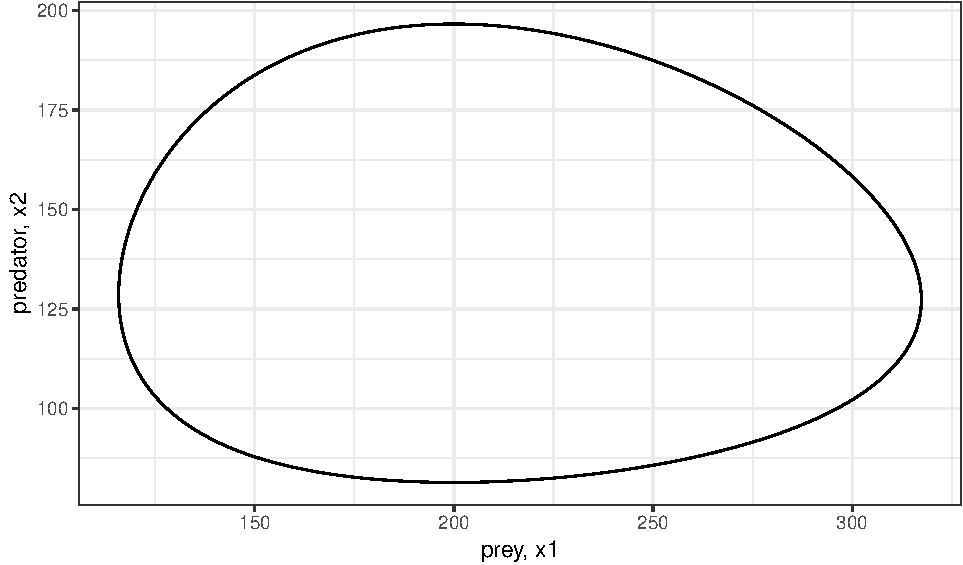
\includegraphics{_myDissertation_files/figure-latex/pp1Period-1.pdf}
\caption{\label{fig:pp1Period}Phase space plot of two-species Lotka-Volterra
predator-prey system over a single period (\textasciitilde{}11.145 time
units.}
\end{figure}
\subsection{Concepts behind the
calculations}\label{concepts-behind-the-calculations}

Although the numerical steps for calculating the derivatives-based FI
are relatively straightforward, the concepts required to interpret the
measure in the context of multiple variables is more complex. Here, we
thoroughly discuss the concepts and assumptions behind FI calculation.
Below, steps do not represent steps within the calculation, they
represent the major concepts required

\subsubsection{\texorpdfstring{\textbf{Step 1. Probability of observing
the system in a particular state,
\(p(x)\)}}{Step 1. Probability of observing the system in a particular state, p(x)}}\label{step-1.-probability-of-observing-the-system-in-a-particular-state-px}
\begin{Shaded}
\begin{Highlighting}[]
\CommentTok{# Plot probability of observing the system in a particular state}
\KeywordTok{ggplot}\NormalTok{(}\DataTypeTok{data =}\NormalTok{ sysSol, }\KeywordTok{aes}\NormalTok{(}\DataTypeTok{x =}\NormalTok{ x1, }\DataTypeTok{y =}\NormalTok{ x2)) }\OperatorTok{+}
\StringTok{  }\KeywordTok{geom_bin2d}\NormalTok{(}\KeywordTok{aes}\NormalTok{(}\DataTypeTok{fill =}\NormalTok{ ..density..), }\DataTypeTok{color =} \StringTok{"black"}\NormalTok{, }\DataTypeTok{drop =}\NormalTok{ T, }\DataTypeTok{bins =} \DecValTok{20}\NormalTok{) }\OperatorTok{+}
\StringTok{  }\KeywordTok{scale_fill_distiller}\NormalTok{(}\DataTypeTok{palette =} \StringTok{"YlOrRd"}\NormalTok{) }\OperatorTok{+}
\StringTok{  }\KeywordTok{labs}\NormalTok{(}\DataTypeTok{x =} \StringTok{"prey, x1"}\NormalTok{, }\DataTypeTok{y =} \StringTok{"predator, x2"}\NormalTok{, }\DataTypeTok{fill =} \StringTok{"p(x)"}\NormalTok{) }\OperatorTok{+}
\StringTok{  }\KeywordTok{coord_fixed}\NormalTok{()}
\end{Highlighting}
\end{Shaded}
\begin{figure}
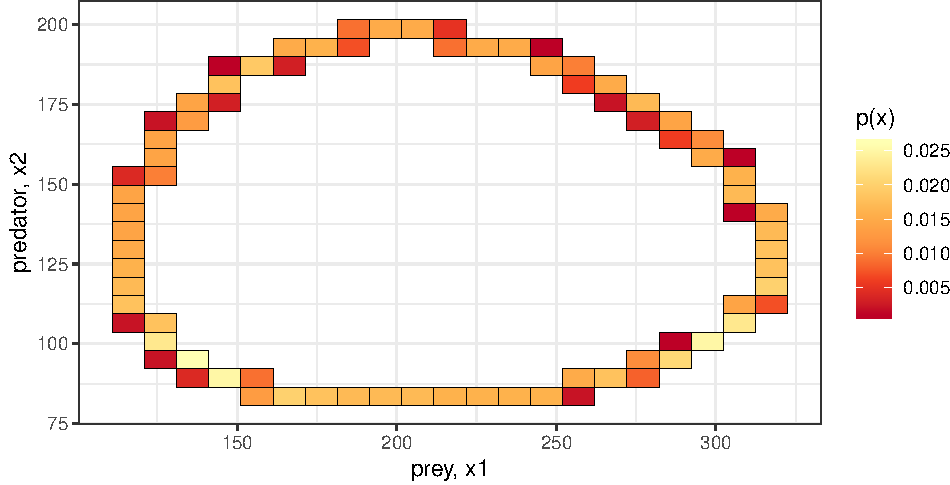
\includegraphics[width=0.85\linewidth]{_myDissertation_files/figure-latex/2D-hist-1} \caption{A 2-dimensional histogram of the probability of observing a system in a particular state, $p(x)$, of the 2-species Lotka-Volterra predator prey system over a single period (~11.145 time units).}\label{fig:2D-hist}
\end{figure}
Fisher Information (FI) is defined with respect to a probability
distribution. In the derivatives-based method, FI is calculated for a
probability of observing a system (as defined by one or more state
variables) in a particular state, \(p(x)\), over some period of time,
(\(0 to t_{end}\)). In other words \(p(x)\) is the probability that, at
a specific point in time (\(t_{obs}^*\)) we will observe the system in a
particular state, \(x^*\). The time at which we observe the system is a
random variable, \(t_{obs} ~ Uniform(0,t_{end})\). To be clear, the
study system is assumed to be deterministic and we assume no observation
error, however, the observed state of the system, \(x(T_{obs})\), is a
random variable because it is a function of the random observation time,
\(x^*= x(t_{obs}^*)\). The state of the model system, x, is defined in
two dimensions by the number of predators and the number of prey
\eqref{eq:predprey} and is easily visualized
\ref{fig:pp1Period}.Therefore, the probability of observing a particular
state is a two-dimensional joint distribution \ref{fig:2d-hist}.

A single state of the model system is defined by the number of predators
and prey at a given point in time such that for any given point in time
\(x(t)=[x_1 (t),x_2 (t)]\). At some random time between 0 and
\(t_{end}\) {[}\(T_{obs} ~ Uniform(0,t_{end})\){]} we can count the
number of predators and the number of prey to determine the state of the
model system. We must assume the system is deterministic and there is no
observation error. We can then calculate the probability of observing a
particular predator and prey abundance combination, \(p(x)\). Under
these assumptions, the only possible states of the system are defined by
the system's observed trajectory, the model parameters, and the initial
conditions. Therefore, the support of the probability distribution
\ref{fig:2D-hist} is the trajectory of the system.
\begin{Shaded}
\begin{Highlighting}[]
\NormalTok{knitr}\OperatorTok{::}\KeywordTok{include_graphics}\NormalTok{(}\StringTok{'./chapterFiles/fiGuide/figures/stringFig.png'}\NormalTok{)}
\end{Highlighting}
\end{Shaded}
\begin{figure}
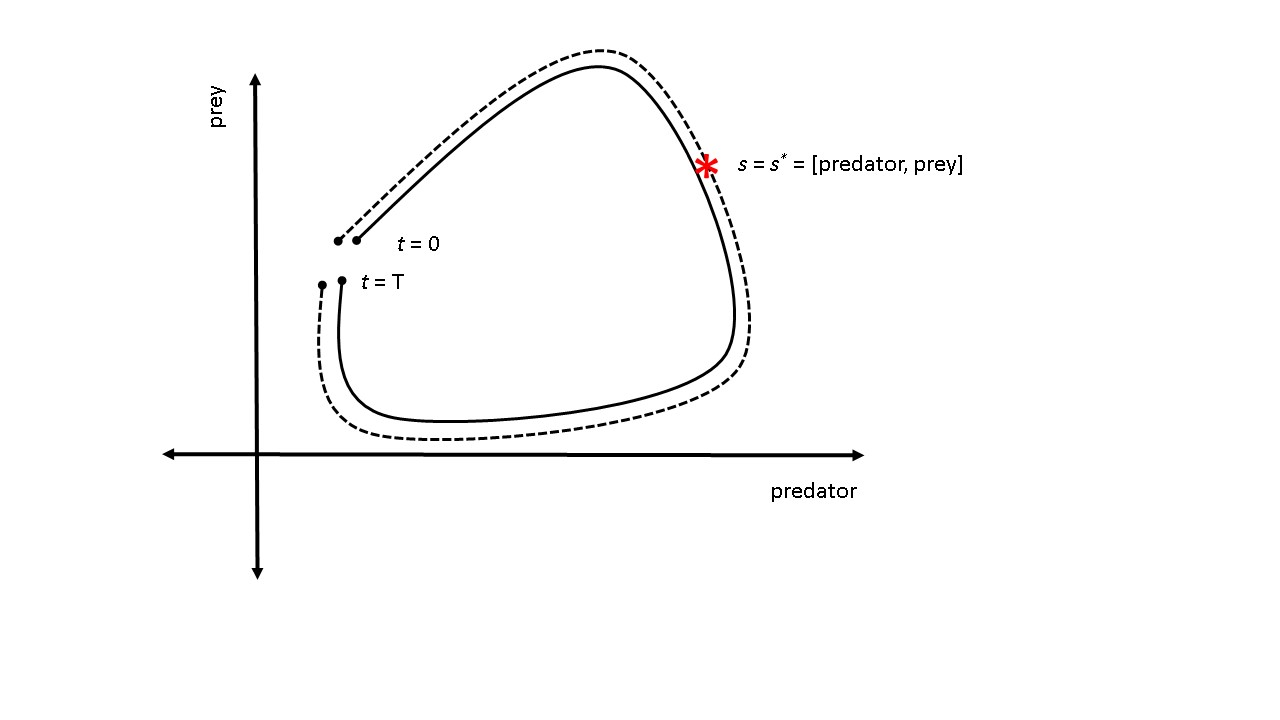
\includegraphics[width=17.78in]{./chapterFiles/fiGuide/figures/stringFig} \caption{A single cycle of a hypothetical two-species system over time period $t = 0$ to $t = T$. $s^*$ is the state of the system at some point in time. The dotted line represents the distance travelled by the system in phase space over its trajectory during time $(0, T)$.}\label{fig:stringFig}
\end{figure}
\subsubsection{\texorpdfstring{\textbf{Step 2.} Distance traveled by the
system,
\(s\)}{Step 2. Distance traveled by the system, s}}\label{step-2.-distance-traveled-by-the-system-s}

Distance traveled by the system, s. We can now move from an
n-dimensional representation of the probability distribution to a
one-dimensional representation. To better understand this, imagine
placing a string over the path of the entire trajectory from
\(0 to t_{end}\) \ref{fig:stringFig}. If we know the number of predators
and prey at a particular point in time \((t_{obs}^*)\) then we can mark
that location on the string (see asterisk in \ref{fig:stringFig}. Next,
imagine picking up the string and laying the string flat along a ruler.
The length, s, of the entire string measures the total distance traveled
by the system in phase space. The mark we made on the string (denoted
\(*\)) lies at a distance \(s^*\) between 0 and \(s\). We call this
length the distance traveled by the system, \(s^*\). In this context,
\(s^*\) in phase space represents a measure of cumulative change in
state. We note that the distance traveled in phase space increases
monotonically with time. If the system never revisits the same state
(i.e., the trajectory never overlaps or intersects itself), then every
unique system state (i.e., point on the trajectory) is mapped to a
unique value of distance traveled. Therefore, \(p(x)\) (n-dimensional)
is equivalent to the probability that the system is at distance s, i.e.,
\(p(x)=p(s)\), (where \(p(s)\) is one dimensional; Cabezas, Pawlowski,
Mayer, \& Hoagland (2005)). However, if the system revisits previous
states, then a unique system state may be mapped to different values of
distance traveled and the relationship between \(p(x)\) and \(p(s)\) is
not one-to-one. We calculated the distance traveled s of the model
system over a single cycle (11.145 time units; \ref{fig:distSpeedAccel}.
\begin{Shaded}
\begin{Highlighting}[]
\CommentTok{# Initial conditions including distance}
\NormalTok{state_highO <-}\StringTok{ }\KeywordTok{c}\NormalTok{(}
  \DataTypeTok{x1 =} \FloatTok{277.7815}\NormalTok{, }
  \DataTypeTok{x2 =} \FloatTok{174.551}\NormalTok{,}
  \DataTypeTok{dx1dt =} \OperatorTok{-}\FloatTok{48.6}\NormalTok{,}
  \DataTypeTok{dx2dt =} \FloatTok{28.3}\NormalTok{,}
  \DataTypeTok{d2x1dt2 =} \OperatorTok{-}\FloatTok{23.3}\NormalTok{,}
  \DataTypeTok{d2x2dt2 =} \OperatorTok{-}\FloatTok{10.5}\NormalTok{,}
  \DataTypeTok{s =} \DecValTok{0}
\NormalTok{)}

\CommentTok{# Model parameters}
\NormalTok{parameters_highO <-}\StringTok{ }\KeywordTok{c}\NormalTok{(}
  \DataTypeTok{g1 =} \DecValTok{1}\NormalTok{,}
  \DataTypeTok{m2 =} \DecValTok{1}\NormalTok{,}
  \DataTypeTok{l12 =} \FloatTok{0.01}\NormalTok{,}
  \DataTypeTok{g21 =} \FloatTok{0.01}\NormalTok{,}
  \DataTypeTok{k =} \DecValTok{625}\NormalTok{,}
  \DataTypeTok{B =} \FloatTok{0.005}
\NormalTok{)}

\CommentTok{# System differential equations including higher order terms and distance}
\NormalTok{deq_highO <-}\StringTok{ }\ControlFlowTok{function}\NormalTok{(t, state, parameters) \{}
  \KeywordTok{with}\NormalTok{(}\KeywordTok{as.list}\NormalTok{(}\KeywordTok{c}\NormalTok{(state, parameters)), \{}
    
  \CommentTok{# 1st derivatives}
\NormalTok{  dx1dt <-}
\StringTok{  }\NormalTok{g1 }\OperatorTok{*}\StringTok{ }\NormalTok{x1 }\OperatorTok{*}\StringTok{ }\NormalTok{(}\DecValTok{1} \OperatorTok{-}\StringTok{ }\NormalTok{(x1 }\OperatorTok{/}\StringTok{ }\NormalTok{k)) }\OperatorTok{-}\StringTok{ }\NormalTok{(l12 }\OperatorTok{*}\StringTok{ }\NormalTok{x1 }\OperatorTok{*}\StringTok{ }\NormalTok{x2) }\OperatorTok{/}\StringTok{ }\NormalTok{(}\DecValTok{1} \OperatorTok{+}\StringTok{ }\NormalTok{B }\OperatorTok{*}\StringTok{ }\NormalTok{x1)}
  
\NormalTok{  dx2dt <-}\StringTok{ }\NormalTok{(g21 }\OperatorTok{*}\StringTok{ }\NormalTok{x1 }\OperatorTok{*}\StringTok{ }\NormalTok{x2) }\OperatorTok{/}\StringTok{ }\NormalTok{(}\DecValTok{1} \OperatorTok{+}\StringTok{ }\NormalTok{B }\OperatorTok{*}\StringTok{ }\NormalTok{x1) }\OperatorTok{-}\StringTok{ }\NormalTok{m2 }\OperatorTok{*}\StringTok{ }\NormalTok{x2}
  
  \CommentTok{# 2nd derivatives}
\NormalTok{  d2x1dt2 <-}
\StringTok{  }\NormalTok{(B }\OperatorTok{*}\StringTok{ }\NormalTok{l12 }\OperatorTok{*}\StringTok{ }\NormalTok{x1 }\OperatorTok{*}\StringTok{ }\NormalTok{x2 }\OperatorTok{*}\StringTok{ }\NormalTok{dx1dt) }\OperatorTok{/}\StringTok{ }\NormalTok{(B }\OperatorTok{*}\StringTok{ }\NormalTok{x1 }\OperatorTok{+}\StringTok{ }\DecValTok{1}\NormalTok{) }\OperatorTok{^}\StringTok{ }\DecValTok{2} \OperatorTok{-}\StringTok{ }\NormalTok{(g1 }\OperatorTok{*}\StringTok{ }\NormalTok{x1 }\OperatorTok{*}\StringTok{ }\NormalTok{dx1dt) }\OperatorTok{/}\StringTok{ }\NormalTok{k }\OperatorTok{-}\StringTok{ }\NormalTok{(l12 }\OperatorTok{*}
\StringTok{  }\NormalTok{x1 }\OperatorTok{*}\StringTok{ }\NormalTok{dx2dt) }\OperatorTok{/}\StringTok{ }\NormalTok{(B }\OperatorTok{*}\StringTok{ }\NormalTok{x1 }\OperatorTok{+}\StringTok{ }\DecValTok{1}\NormalTok{) }\OperatorTok{-}\StringTok{ }\NormalTok{(l12 }\OperatorTok{*}\StringTok{ }\NormalTok{x2 }\OperatorTok{*}\StringTok{ }\NormalTok{dx1dt) }\OperatorTok{/}\StringTok{ }\NormalTok{(B }\OperatorTok{*}\StringTok{ }\NormalTok{x1 }\OperatorTok{+}\StringTok{ }\DecValTok{1}\NormalTok{) }\OperatorTok{-}\StringTok{ }\NormalTok{g1 }\OperatorTok{*}\StringTok{ }\NormalTok{(x1 }\OperatorTok{/}
\StringTok{  }\NormalTok{k }\OperatorTok{-}\StringTok{ }\DecValTok{1}\NormalTok{) }\OperatorTok{*}\StringTok{ }\NormalTok{dx1dt}
  
\NormalTok{  d2x2dt2 <-}
\StringTok{  }\NormalTok{(g21 }\OperatorTok{*}\StringTok{ }\NormalTok{x1 }\OperatorTok{*}\StringTok{ }\NormalTok{dx2dt) }\OperatorTok{/}\StringTok{ }\NormalTok{(B }\OperatorTok{*}\StringTok{ }\NormalTok{x1 }\OperatorTok{+}\StringTok{ }\DecValTok{1}\NormalTok{) }\OperatorTok{-}\StringTok{ }\NormalTok{m2 }\OperatorTok{*}\StringTok{ }\NormalTok{dx2dt }\OperatorTok{+}\StringTok{ }\NormalTok{(g21 }\OperatorTok{*}\StringTok{ }\NormalTok{x2 }\OperatorTok{*}\StringTok{ }\NormalTok{dx1dt) }\OperatorTok{/}\StringTok{ }\NormalTok{(B }\OperatorTok{*}
\StringTok{  }\NormalTok{x1 }\OperatorTok{+}\StringTok{ }\DecValTok{1}\NormalTok{) }\OperatorTok{-}\StringTok{ }\NormalTok{(B }\OperatorTok{*}\StringTok{ }\NormalTok{g21 }\OperatorTok{*}\StringTok{ }\NormalTok{x1 }\OperatorTok{*}\StringTok{ }\NormalTok{x2 }\OperatorTok{*}\StringTok{ }\NormalTok{dx1dt) }\OperatorTok{/}\StringTok{ }\NormalTok{(B }\OperatorTok{*}\StringTok{ }\NormalTok{x1 }\OperatorTok{+}\StringTok{ }\DecValTok{1}\NormalTok{) }\OperatorTok{^}\StringTok{ }\DecValTok{2}
  
  \CommentTok{# 3rd derivatives}
\NormalTok{  d3x1dt3 <-}
\StringTok{  }\NormalTok{(}\DecValTok{2} \OperatorTok{*}\StringTok{ }\NormalTok{B }\OperatorTok{*}\StringTok{ }\NormalTok{l12 }\OperatorTok{*}\StringTok{ }\NormalTok{x2 }\OperatorTok{*}\StringTok{ }\NormalTok{dx1dt }\OperatorTok{^}\StringTok{ }\DecValTok{2}\NormalTok{) }\OperatorTok{/}\StringTok{ }\NormalTok{(B }\OperatorTok{*}\StringTok{ }\NormalTok{x1 }\OperatorTok{+}\StringTok{ }\DecValTok{1}\NormalTok{) }\OperatorTok{^}\StringTok{ }\DecValTok{2} \OperatorTok{-}\StringTok{ }\NormalTok{(}\DecValTok{2} \OperatorTok{*}\StringTok{ }\NormalTok{g1 }\OperatorTok{*}\StringTok{ }\NormalTok{dx1dt }\OperatorTok{^}\StringTok{ }\DecValTok{2}\NormalTok{) }\OperatorTok{/}
\StringTok{  }\NormalTok{k }\OperatorTok{-}\StringTok{ }\NormalTok{(l12 }\OperatorTok{*}\StringTok{ }\NormalTok{x1 }\OperatorTok{*}\StringTok{ }\NormalTok{d2x2dt2) }\OperatorTok{/}\StringTok{ }\NormalTok{(B }\OperatorTok{*}\StringTok{ }\NormalTok{x1 }\OperatorTok{+}\StringTok{ }\DecValTok{1}\NormalTok{) }\OperatorTok{-}\StringTok{ }\NormalTok{(l12 }\OperatorTok{*}\StringTok{ }\NormalTok{x2 }\OperatorTok{*}\StringTok{ }\NormalTok{d2x1dt2) }\OperatorTok{/}\StringTok{ }\NormalTok{(B }\OperatorTok{*}\StringTok{ }\NormalTok{x1 }\OperatorTok{+}\StringTok{ }\DecValTok{1}\NormalTok{) }\OperatorTok{-}\StringTok{ }\NormalTok{(}\DecValTok{2} \OperatorTok{*}
\StringTok{  }\NormalTok{l12 }\OperatorTok{*}\StringTok{ }\NormalTok{dx1dt }\OperatorTok{*}\StringTok{ }\NormalTok{dx2dt) }\OperatorTok{/}\StringTok{ }\NormalTok{(B }\OperatorTok{*}\StringTok{ }\NormalTok{x1 }\OperatorTok{+}\StringTok{ }\DecValTok{1}\NormalTok{) }\OperatorTok{-}\StringTok{ }\NormalTok{(g1 }\OperatorTok{*}\StringTok{ }\NormalTok{x1 }\OperatorTok{*}\StringTok{ }\NormalTok{d2x1dt2) }\OperatorTok{/}\StringTok{ }\NormalTok{k }\OperatorTok{-}\StringTok{ }\NormalTok{g1 }\OperatorTok{*}\StringTok{ }\NormalTok{(x1 }\OperatorTok{/}
\StringTok{  }\NormalTok{k }\OperatorTok{-}\StringTok{ }\DecValTok{1}\NormalTok{) }\OperatorTok{*}\StringTok{ }\NormalTok{d2x1dt2 }\OperatorTok{+}\StringTok{ }\NormalTok{(B }\OperatorTok{*}\StringTok{ }\NormalTok{l12 }\OperatorTok{*}\StringTok{ }\NormalTok{x1 }\OperatorTok{*}\StringTok{ }\NormalTok{x2 }\OperatorTok{*}\StringTok{ }\NormalTok{d2x1dt2) }\OperatorTok{/}\StringTok{ }\NormalTok{(B }\OperatorTok{*}\StringTok{ }\NormalTok{x1 }\OperatorTok{+}\StringTok{ }\DecValTok{1}\NormalTok{) }\OperatorTok{^}\StringTok{ }\DecValTok{2} \OperatorTok{-}\StringTok{ }\NormalTok{(}\DecValTok{2} \OperatorTok{*}
\StringTok{  }\NormalTok{B }\OperatorTok{^}\StringTok{ }\DecValTok{2} \OperatorTok{*}\StringTok{ }\NormalTok{l12 }\OperatorTok{*}\StringTok{ }\NormalTok{x1 }\OperatorTok{*}\StringTok{ }\NormalTok{x2 }\OperatorTok{*}\StringTok{ }\NormalTok{dx1dt }\OperatorTok{^}\StringTok{ }\DecValTok{2}\NormalTok{) }\OperatorTok{/}\StringTok{ }\NormalTok{(B }\OperatorTok{*}\StringTok{ }\NormalTok{x1 }\OperatorTok{+}\StringTok{ }\DecValTok{1}\NormalTok{) }\OperatorTok{^}\StringTok{ }\DecValTok{3} \OperatorTok{+}\StringTok{ }\NormalTok{(}\DecValTok{2} \OperatorTok{*}\StringTok{ }\NormalTok{B }\OperatorTok{*}\StringTok{ }\NormalTok{l12 }\OperatorTok{*}\StringTok{ }\NormalTok{x1 }\OperatorTok{*}
\StringTok{  }\NormalTok{dx1dt }\OperatorTok{*}\StringTok{ }\NormalTok{dx2dt) }\OperatorTok{/}\StringTok{ }\NormalTok{(B }\OperatorTok{*}\StringTok{ }\NormalTok{x1 }\OperatorTok{+}\StringTok{ }\DecValTok{1}\NormalTok{) }\OperatorTok{^}\StringTok{ }\DecValTok{2}
  
\NormalTok{  d3x2dt3 <-}
\StringTok{  }\NormalTok{(g21 }\OperatorTok{*}\StringTok{ }\NormalTok{x1 }\OperatorTok{*}\StringTok{ }\NormalTok{d2x2dt2) }\OperatorTok{/}\StringTok{ }\NormalTok{(B }\OperatorTok{*}\StringTok{ }\NormalTok{x1 }\OperatorTok{+}\StringTok{ }\DecValTok{1}\NormalTok{) }\OperatorTok{-}\StringTok{ }\NormalTok{m2 }\OperatorTok{*}\StringTok{ }\NormalTok{d2x2dt2 }\OperatorTok{+}\StringTok{ }\NormalTok{(g21 }\OperatorTok{*}\StringTok{ }\NormalTok{x2 }\OperatorTok{*}\StringTok{ }\NormalTok{d2x1dt2) }\OperatorTok{/}
\StringTok{  }\NormalTok{(B }\OperatorTok{*}\StringTok{ }\NormalTok{x1 }\OperatorTok{+}\StringTok{ }\DecValTok{1}\NormalTok{) }\OperatorTok{+}\StringTok{ }\NormalTok{(}\DecValTok{2} \OperatorTok{*}\StringTok{ }\NormalTok{g21 }\OperatorTok{*}\StringTok{ }\NormalTok{dx1dt }\OperatorTok{*}\StringTok{ }\NormalTok{dx2dt) }\OperatorTok{/}\StringTok{ }\NormalTok{(B }\OperatorTok{*}\StringTok{ }\NormalTok{x1 }\OperatorTok{+}\StringTok{ }\DecValTok{1}\NormalTok{) }\OperatorTok{-}\StringTok{ }\NormalTok{(}\DecValTok{2} \OperatorTok{*}\StringTok{ }\NormalTok{B }\OperatorTok{*}\StringTok{ }\NormalTok{g21 }\OperatorTok{*}
\StringTok{  }\NormalTok{x2 }\OperatorTok{*}\StringTok{ }\NormalTok{dx1dt }\OperatorTok{^}\StringTok{ }\DecValTok{2}\NormalTok{) }\OperatorTok{/}\StringTok{ }\NormalTok{(B }\OperatorTok{*}\StringTok{ }\NormalTok{x1 }\OperatorTok{+}\StringTok{ }\DecValTok{1}\NormalTok{) }\OperatorTok{^}\StringTok{ }\DecValTok{2} \OperatorTok{-}\StringTok{ }\NormalTok{(B }\OperatorTok{*}\StringTok{ }\NormalTok{g21 }\OperatorTok{*}\StringTok{ }\NormalTok{x1 }\OperatorTok{*}\StringTok{ }\NormalTok{x2 }\OperatorTok{*}\StringTok{ }\NormalTok{d2x1dt2) }\OperatorTok{/}\StringTok{ }\NormalTok{(B }\OperatorTok{*}
\StringTok{  }\NormalTok{x1 }\OperatorTok{+}\StringTok{ }\DecValTok{1}\NormalTok{) }\OperatorTok{^}\StringTok{ }\DecValTok{2} \OperatorTok{+}\StringTok{ }\NormalTok{(}\DecValTok{2} \OperatorTok{*}\StringTok{ }\NormalTok{B }\OperatorTok{^}\StringTok{ }\DecValTok{2} \OperatorTok{*}\StringTok{ }\NormalTok{g21 }\OperatorTok{*}\StringTok{ }\NormalTok{x1 }\OperatorTok{*}\StringTok{ }\NormalTok{x2 }\OperatorTok{*}\StringTok{ }\NormalTok{dx1dt }\OperatorTok{^}\StringTok{ }\DecValTok{2}\NormalTok{) }\OperatorTok{/}\StringTok{ }\NormalTok{(B }\OperatorTok{*}\StringTok{ }\NormalTok{x1 }\OperatorTok{+}\StringTok{ }\DecValTok{1}\NormalTok{) }\OperatorTok{^}\StringTok{ }\DecValTok{3} \OperatorTok{-}\StringTok{ }\NormalTok{(}\DecValTok{2} \OperatorTok{*}
\StringTok{  }\NormalTok{B }\OperatorTok{*}\StringTok{ }\NormalTok{g21 }\OperatorTok{*}\StringTok{ }\NormalTok{x1 }\OperatorTok{*}\StringTok{ }\NormalTok{dx1dt }\OperatorTok{*}\StringTok{ }\NormalTok{dx2dt) }\OperatorTok{/}\StringTok{ }\NormalTok{(B }\OperatorTok{*}\StringTok{ }\NormalTok{x1 }\OperatorTok{+}\StringTok{ }\DecValTok{1}\NormalTok{) }\OperatorTok{^}\StringTok{ }\DecValTok{2}
  
  \CommentTok{# Derivative of distance (i.e., tangential velocity)}
\NormalTok{  dsdt <-}\StringTok{ }\KeywordTok{sqrt}\NormalTok{(dx1dt }\OperatorTok{^}\StringTok{ }\DecValTok{2} \OperatorTok{+}\StringTok{ }\NormalTok{dx2dt }\OperatorTok{^}\StringTok{ }\DecValTok{2}\NormalTok{)}
  
  \KeywordTok{list}\NormalTok{(}\KeywordTok{c}\NormalTok{(dx1dt, dx2dt, d2x1dt2, d2x2dt2, d3x1dt3, d3x2dt3, dsdt))}
\NormalTok{  \})}
\NormalTok{\}}

\CommentTok{# Solve system differential equations (now with distance)}
\NormalTok{out_highO <-}\StringTok{ }\KeywordTok{ode}\NormalTok{(}
  \DataTypeTok{y =}\NormalTok{ state_highO,}
  \DataTypeTok{times =}\NormalTok{ times,}
  \DataTypeTok{func =}\NormalTok{ deq_highO,}
  \DataTypeTok{parms =}\NormalTok{ parameters_highO,}
  \DataTypeTok{rtol =} \FloatTok{1e-10}\NormalTok{,}
  \DataTypeTok{method =} \StringTok{"ode45"}
\NormalTok{)}

\CommentTok{# Convert to data frame}
\NormalTok{sysSol_highO <-}
\StringTok{  }\KeywordTok{tibble}\NormalTok{(}\DataTypeTok{t =}\NormalTok{ out_highO[, }\DecValTok{1}\NormalTok{],}
             \DataTypeTok{x1 =}\NormalTok{ out_highO[, }\DecValTok{2}\NormalTok{],}
             \DataTypeTok{x2 =}\NormalTok{ out_highO[, }\DecValTok{3}\NormalTok{],}
             \DataTypeTok{dx1dt =}\NormalTok{ out_highO[,}\DecValTok{4}\NormalTok{],}
             \DataTypeTok{dx2dt =}\NormalTok{ out_highO[,}\DecValTok{5}\NormalTok{],}
             \DataTypeTok{d2x1dt2 =}\NormalTok{ out_highO[,}\DecValTok{6}\NormalTok{],}
             \DataTypeTok{d2x2dt2 =}\NormalTok{ out_highO[,}\DecValTok{7}\NormalTok{],}
             \DataTypeTok{s =}\NormalTok{ out_highO[, }\DecValTok{8}\NormalTok{]) }\OperatorTok\StringTok{  }
\StringTok{  }\CommentTok{# Calculate derivatives and pdf}
\StringTok{  }\KeywordTok{mutate}\NormalTok{(}\DataTypeTok{dsdt =} \KeywordTok{sqrt}\NormalTok{(dx1dt}\OperatorTok{^}\DecValTok{2} \OperatorTok{+}\StringTok{ }\NormalTok{dx2dt}\OperatorTok{^}\DecValTok{2}\NormalTok{),}
         \DataTypeTok{d2sdt2 =}\NormalTok{ (}\DecValTok{1}\OperatorTok{/}\NormalTok{dsdt)}\OperatorTok{*}\NormalTok{(dx1dt}\OperatorTok{*}\NormalTok{d2x1dt2 }\OperatorTok{+}\StringTok{ }\NormalTok{dx2dt}\OperatorTok{*}\NormalTok{d2x2dt2),}
         \DataTypeTok{p =}\NormalTok{ (}\DecValTok{1}\OperatorTok{/}\NormalTok{TT)}\OperatorTok{*}\NormalTok{(}\DecValTok{1}\OperatorTok{/}\NormalTok{dsdt))}
\end{Highlighting}
\end{Shaded}
\begin{Shaded}
\begin{Highlighting}[]
\CommentTok{# Plot distance traveled}
\NormalTok{p1 <-}\StringTok{ }\KeywordTok{ggplot}\NormalTok{(}\DataTypeTok{data =}\NormalTok{ sysSol_highO, }\KeywordTok{aes}\NormalTok{(}\DataTypeTok{x =}\NormalTok{ t, }\DataTypeTok{y =}\NormalTok{ s)) }\OperatorTok{+}
\StringTok{  }\KeywordTok{geom_line}\NormalTok{() }\OperatorTok{+}
\StringTok{  }\KeywordTok{labs}\NormalTok{(}\DataTypeTok{x =} \StringTok{"time"}\NormalTok{, }\DataTypeTok{y =} \StringTok{"distance"}\NormalTok{)}

\CommentTok{# Plot velocity}
\NormalTok{p2 <-}\StringTok{ }\KeywordTok{ggplot}\NormalTok{(}\DataTypeTok{data =}\NormalTok{ sysSol_highO, }\KeywordTok{aes}\NormalTok{(}\DataTypeTok{x =}\NormalTok{ t, }\DataTypeTok{y =}\NormalTok{ dsdt)) }\OperatorTok{+}
\StringTok{  }\KeywordTok{geom_line}\NormalTok{() }\OperatorTok{+}
\StringTok{  }\KeywordTok{labs}\NormalTok{(}\DataTypeTok{x =} \StringTok{"time"}\NormalTok{, }\DataTypeTok{y =} \StringTok{"speed"}\NormalTok{)}

\CommentTok{# Plot acceleration}
\NormalTok{p3 <-}\StringTok{ }\KeywordTok{ggplot}\NormalTok{(}\DataTypeTok{data =}\NormalTok{ sysSol_highO, }\KeywordTok{aes}\NormalTok{(}\DataTypeTok{x =}\NormalTok{ t, }\DataTypeTok{y =}\NormalTok{ d2sdt2)) }\OperatorTok{+}
\StringTok{  }\KeywordTok{geom_line}\NormalTok{() }\OperatorTok{+}
\StringTok{  }\KeywordTok{labs}\NormalTok{(}\DataTypeTok{x =} \StringTok{"time"}\NormalTok{, }\DataTypeTok{y =} \StringTok{"acceleration"}\NormalTok{)}

\CommentTok{# Grid plot}
\NormalTok{gridExtra}\OperatorTok{::}\KeywordTok{grid.arrange}\NormalTok{(p1, p2, p3, }\DataTypeTok{ncol=}\DecValTok{1}\NormalTok{)}
\end{Highlighting}
\end{Shaded}
\begin{figure}
\centering
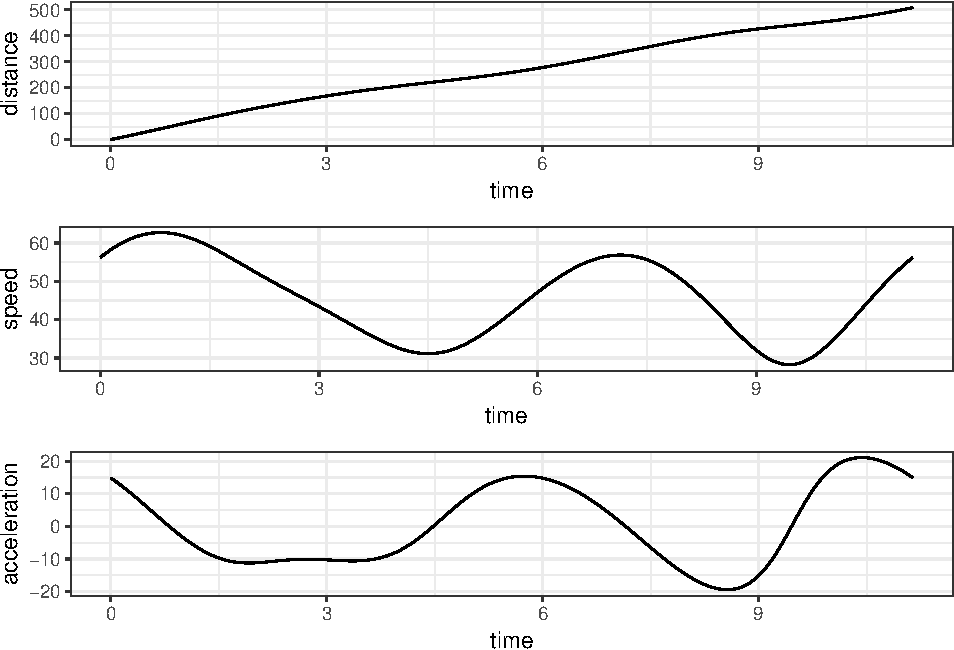
\includegraphics{_myDissertation_files/figure-latex/distSpeedAccel-1.pdf}
\caption{\label{fig:distSpeedAccel}From top to bottom, distance traveled in
phase space, speed tangential to system trajectory, acceleration
tangential to system trajectory.}
\end{figure}
\subsubsection{\texorpdfstring{\textbf{Step 3.} \(p(s)\) as a function
of the rate of change of
\(s\)}{Step 3. p(s) as a function of the rate of change of s}}\label{step-3.-ps-as-a-function-of-the-rate-of-change-of-s}

In previous presentations of FI, the relationship between the state of
the system (n-dimensional) and the distance traveled (1-dimensional) was
not always emphasized (Cabezas \& Fath, 2002). Here we use x to denote
the state of the system and s to denote the distance traveled to
emphasize this distinction. If a system travels at a constant speed over
the entire time period, then the system is equally likely to be in any
state along the trajectory (\(s\) is linear and \(p(s)\) is uniform).
Referring to our model system, if the number of predators and prey are
linearly related, then the speed of the system is constant. For
non-linear systems, the distribution above the string will not be
uniform \ref{fig:stringFig}. Rather, it will change depending on the
amount of time the system spends in each state. It follows that \(p(s)\)
is proportional to the inverse of the rate of change of distance
traveled (i.e., the speed along the path in phase space).

We will now demonstrate this using our model system as an example.
Suppose the abundances of the predator and their prey in our model
system predictably operate at carrying capacity. Over a relatively short
period of time the prey abundance quickly declines after a severe
weather event (a pulse disturbance; (Bender et al. 1984), but quickly
recovers. Intuitively, the absolute rate of change at time points near
the disturbance will be larger than during time periods long before or
long after the disturbance. It is therefore more likely that the system
will be (observed) in a state where prey and predators are operating
approximately at carrying capacity than in a state with relatively low
prey abundance. Mathematically, the time, \(t*\), at which we calculate
the abundances of prey and predators is a uniform random variable, and
the distance traveled by the system, \(s^*\), is a function of time, is
differentiable, and monotonically increases. Therefore, the probability
density function of the distance traveled
\(p(s)=\frac{1}{T}\frac{1}{s'}\), where \(s'= \frac{ds}{dt}\) is the
speed of the system (the speed tangential to the trajectory; the first
derivative of the distance traveled; instantaneous rate of change of
\(s\)). We calculated the speed (the first derivative;
\ref{fig:distSpeedAccel} and acceleration (the second derivative;
\ref{fig:distSpeedAccel} of the distance traveled s by the model system
over a single cycle using function ode in package deSolve (Soetaert et
al. 2010) in Program R (R Core Team 2016).

\subsubsection{\texorpdfstring{\textbf{Step 4.} Calculate the
derivatives-based Fisher
Information}{Step 4. Calculate the derivatives-based Fisher Information}}\label{step-4.-calculate-the-derivatives-based-fisher-information}

Now that we understand how to calculate both the distance traveled,
\(s\), and its probability density, \(p(s)\), calculating the
derivatives-based FI is straightforward and computationally inexpensive
\eqref{eq:fiDerivs}. There are several comparable equations for
calculating the shift-invariant FI, and some may offer numerical
advantages over others. Equation \eqref{eq:fiAdapted} is the general form
and Equation \eqref{eq:fi73c} is the amplitude form for FI (in D. A. L.
Mayer et al. (2007), respectively). Although these formulations are
equivalent, \eqref{eq:fi73c} is most readily calculated when the
differential equations for the system are known, obviating any advantage
of a model-free metric.
\begin{equation}   
    I = \frac{1}{T} \int_0^T dt\left[\frac{s''^2}{s'^4}\right]^2 \\  
  \label{eq:fiDerivs}  
\end{equation}
\begin{equation} 
    I = \int \frac{ds}{p(s)}\left[\frac{dp(s)}{ds}\right]^2  \\
    \label{eq:fiAdapted}
\end{equation}
\begin{equation} 
    I = 4 \int ds\left[\frac{dq(s)}{ds}\right]^2 \\
\label{eq:fi73c}
\end{equation}
This article is interested in the Fisher Information calculated for a
distribution of distance traveled, \(s\), by the entire system. We
calculated the Fisher Information value using Equation \eqref{eq:fiDerivs}
over a single period of the model system (\eqref{eq:predprey}). We
calculated Fisher Information to be \(5.3\) x \(10^{-5}\) which is
consistent with the results of Mayer et al. (2007).

\section{Case Study}\label{case-study}

Mayer et al. (2007) calculated FI for a predator-prey system for several
discrete values of carrying capacity of prey. The results of this study
showed that FI was different for systems with different carrying
capacities. However, this study did not address the central question of
how FI changes during a regime shift. As an extension of the original
study, we simulate a regime shift by modeling a situation where carrying
capacity is abruptly decreased. To simulate an abrupt change in carrying
capacity, we assume carrying capacity is described by Eq. 6 where \(k1\)
is the initial carrying capacity, \(k2\) is the final carrying capacity,
\(t*\) is the time of the regime shift, and alpha is a parameter that
controls how quickly the regime shift occurs. The hyperbolic tangent
function simulates a smooth, continuous change in carrying capacity
while still allowing for the change to occur suddenly. To incorporate
the change in carrying capacity into the system differential equations
we define the rate of change of carrying capacity as given by
\eqref{eq:mayerCase}.\\
\begin{equation}  
  k(t) = k_1  - 0.5(k_1-k_2)(\tanh(\alpha (t-t^*))+1)     \\
  k'(t) = 0.5\alpha (k_1-k_2)(\tanh(\alpha(t-t^*))^2 +1)      \\ 
\label{eq:mayerCase}
\end{equation}
\begin{Shaded}
\begin{Highlighting}[]
\CommentTok{# Equation 7.3b}
\NormalTok{p <-}\StringTok{ }\NormalTok{sysSol_highO}\OperatorTok{$}\NormalTok{p}
\NormalTok{s <-}\StringTok{ }\NormalTok{sysSol_highO}\OperatorTok{$}\NormalTok{s}
\NormalTok{dp <-}\StringTok{ }\KeywordTok{lead}\NormalTok{(p)}\OperatorTok{-}\NormalTok{p}
\NormalTok{ds <-}\StringTok{ }\KeywordTok{lead}\NormalTok{(s)}\OperatorTok{-}\NormalTok{s}
\NormalTok{dpds <-}\StringTok{ }\NormalTok{dp}\OperatorTok{/}\NormalTok{ds}
\NormalTok{ind <-}\StringTok{ }\DecValTok{1}\OperatorTok{:}\NormalTok{(}\KeywordTok{length}\NormalTok{(s)}\OperatorTok{-}\DecValTok{1}\NormalTok{)}
\NormalTok{FI_}\FloatTok{7.}\NormalTok{3b <-}\StringTok{ }\NormalTok{caTools}\OperatorTok{::}\KeywordTok{trapz}\NormalTok{(s[ind], (}\DecValTok{1}\OperatorTok{/}\NormalTok{p[ind])}\OperatorTok{*}\NormalTok{dpds[ind]}\OperatorTok{^}\DecValTok{2}\NormalTok{)}

\CommentTok{# Equation 7.3c}
\NormalTok{q <-}\StringTok{ }\KeywordTok{sqrt}\NormalTok{(sysSol_highO}\OperatorTok{$}\NormalTok{p)}
\NormalTok{s <-}\StringTok{ }\NormalTok{sysSol_highO}\OperatorTok{$}\NormalTok{s}
\NormalTok{dq <-}\StringTok{ }\KeywordTok{lead}\NormalTok{(q)}\OperatorTok{-}\NormalTok{q}
\NormalTok{ds <-}\StringTok{ }\KeywordTok{lead}\NormalTok{(s)}\OperatorTok{-}\NormalTok{s}
\NormalTok{dqds <-}\StringTok{ }\NormalTok{dq}\OperatorTok{/}\NormalTok{ds}
\NormalTok{ind <-}\StringTok{ }\DecValTok{1}\OperatorTok{:}\NormalTok{(}\KeywordTok{length}\NormalTok{(s)}\OperatorTok{-}\DecValTok{1}\NormalTok{)}
\NormalTok{FI_}\FloatTok{7.}\NormalTok{3c <-}\StringTok{ }\DecValTok{4}\OperatorTok{*}\NormalTok{caTools}\OperatorTok{::}\KeywordTok{trapz}\NormalTok{(s[ind], dqds[ind]}\OperatorTok{^}\DecValTok{2}\NormalTok{)}

\CommentTok{# Equation 7.12}
\NormalTok{t <-}\StringTok{ }\NormalTok{sysSol_highO}\OperatorTok{$}\NormalTok{t}
\NormalTok{dsdt <-}\StringTok{ }\NormalTok{sysSol_highO}\OperatorTok{$}\NormalTok{dsdt}
\NormalTok{d2sdt2 <-}\StringTok{ }\NormalTok{sysSol_highO}\OperatorTok{$}\NormalTok{d2sdt2}
\NormalTok{ind <-}\StringTok{ }\DecValTok{1}\OperatorTok{:}\NormalTok{(}\KeywordTok{length}\NormalTok{(s)}\OperatorTok{-}\DecValTok{1}\NormalTok{)}
\NormalTok{FI_}\FloatTok{7.12}\NormalTok{ <-}\StringTok{ }\NormalTok{(}\DecValTok{1}\OperatorTok{/}\NormalTok{TT)}\OperatorTok{*}\NormalTok{caTools}\OperatorTok{::}\KeywordTok{trapz}\NormalTok{(t[ind], d2sdt2}\OperatorTok{^}\DecValTok{2} \OperatorTok{/}\StringTok{ }\NormalTok{dsdt}\OperatorTok{^}\DecValTok{4}\NormalTok{)}

\CommentTok{# Results}
\CommentTok{# FI_7.3b}
\CommentTok{# FI_7.3c}
\CommentTok{# FI_7.12}
\end{Highlighting}
\end{Shaded}
\begin{Shaded}
\begin{Highlighting}[]
\CommentTok{# Carrying capacity}
\NormalTok{k <-}\StringTok{ }\KeywordTok{seq}\NormalTok{(}\DecValTok{625}\NormalTok{, }\DecValTok{800}\NormalTok{, }\DataTypeTok{by =} \DecValTok{25}\NormalTok{)}

\CommentTok{# Initial conditions}
\NormalTok{x1_ini <-}\StringTok{ }\KeywordTok{c}\NormalTok{(}\FloatTok{277.7815}\NormalTok{,}
          \FloatTok{314.6527}\NormalTok{,}
          \FloatTok{303.6386}\NormalTok{,}
          \FloatTok{175.4664}\NormalTok{,}
          \FloatTok{50.72788}\NormalTok{,}
          \FloatTok{135.6263}\NormalTok{,}
          \FloatTok{571.6995}\NormalTok{,}
          \FloatTok{166.9751}\NormalTok{)}
\NormalTok{x2_ini <-}\StringTok{ }\KeywordTok{c}\NormalTok{(}\FloatTok{174.551}\NormalTok{,}
          \FloatTok{191.5272}\NormalTok{,}
          \FloatTok{226.0233}\NormalTok{,}
          \FloatTok{270.6772}\NormalTok{,}
          \FloatTok{133.5784}\NormalTok{,}
          \FloatTok{32.24493}\NormalTok{,}
          \FloatTok{65.22751}\NormalTok{,}
          \FloatTok{345.6978}\NormalTok{)}

\CommentTok{# Loop over k's}
\NormalTok{results_kstudy <-}\StringTok{ }\OtherTok{NULL}
\NormalTok{FI_}\FloatTok{7.}\NormalTok{3b <-}\StringTok{ }\OtherTok{NULL}
\ControlFlowTok{for}\NormalTok{(i }\ControlFlowTok{in} \DecValTok{1}\OperatorTok{:}\KeywordTok{length}\NormalTok{(k))\{}
  
  \CommentTok{# Update parameters}
\NormalTok{  parameters[}\StringTok{"k"}\NormalTok{] <-}\StringTok{ }\NormalTok{k[i]}
\NormalTok{  state[}\StringTok{"x1"}\NormalTok{] <-}\StringTok{ }\NormalTok{x1_ini[i]}
\NormalTok{  state[}\StringTok{"x2"}\NormalTok{] <-}\StringTok{ }\NormalTok{x2_ini[i]}
\NormalTok{  state[}\StringTok{"s"}\NormalTok{] =}\StringTok{ }\DecValTok{0}
  
  \CommentTok{# System differential equations including higher order terms and distance}
\NormalTok{  deq_kstudy <-}\StringTok{ }\ControlFlowTok{function}\NormalTok{(t, state, parameters) \{}
    \KeywordTok{with}\NormalTok{(}\KeywordTok{as.list}\NormalTok{(}\KeywordTok{c}\NormalTok{(state, parameters)), \{}
\NormalTok{      dx1dt <-}\StringTok{ }\NormalTok{g1 }\OperatorTok{*}\StringTok{ }\NormalTok{x1 }\OperatorTok{*}\StringTok{ }\NormalTok{(}\DecValTok{1} \OperatorTok{-}\StringTok{ }\NormalTok{(x1 }\OperatorTok{/}\StringTok{ }\NormalTok{k)) }\OperatorTok{-}\StringTok{ }\NormalTok{(l12 }\OperatorTok{*}\StringTok{ }\NormalTok{x1 }\OperatorTok{*}\StringTok{ }\NormalTok{x2) }\OperatorTok{/}\StringTok{ }\NormalTok{(}\DecValTok{1} \OperatorTok{+}\StringTok{ }\NormalTok{B }\OperatorTok{*}\StringTok{ }\NormalTok{x1)}
      
\NormalTok{      dx2dt <-}\StringTok{ }\NormalTok{(g21 }\OperatorTok{*}\StringTok{ }\NormalTok{x1 }\OperatorTok{*}\StringTok{ }\NormalTok{x2) }\OperatorTok{/}\StringTok{ }\NormalTok{(}\DecValTok{1} \OperatorTok{+}\StringTok{ }\NormalTok{B }\OperatorTok{*}\StringTok{ }\NormalTok{x1) }\OperatorTok{-}\StringTok{ }\NormalTok{m2 }\OperatorTok{*}\StringTok{ }\NormalTok{x2}
      
\NormalTok{      dsdt <-}\StringTok{ }\KeywordTok{sqrt}\NormalTok{(dx1dt}\OperatorTok{^}\DecValTok{2} \OperatorTok{+}\StringTok{ }\NormalTok{dx2dt}\OperatorTok{^}\DecValTok{2}\NormalTok{)}
      
      \KeywordTok{list}\NormalTok{(}\KeywordTok{c}\NormalTok{(dx1dt, dx2dt, dsdt))}
\NormalTok{    \})}
\NormalTok{  \}}
  
  \CommentTok{# Vector of times}
\NormalTok{  TT <-}\StringTok{  }\FloatTok{13.1}
\NormalTok{  times <-}\StringTok{ }\KeywordTok{seq}\NormalTok{(}\DecValTok{0}\NormalTok{, TT, }\DataTypeTok{by =}\NormalTok{ TT}\OperatorTok{/}\FloatTok{1e3}\NormalTok{)}
  
  \CommentTok{# Solve system differential equations (now with distance)}
\NormalTok{  out_kstudy <-}\StringTok{ }\KeywordTok{ode}\NormalTok{(}
    \DataTypeTok{y =}\NormalTok{ state,}
    \DataTypeTok{times =}\NormalTok{ times,}
    \DataTypeTok{func =}\NormalTok{ deq_kstudy,}
    \DataTypeTok{parms =}\NormalTok{ parameters,}
    \DataTypeTok{rtol =} \FloatTok{1e-10}\NormalTok{,}
    \DataTypeTok{method =} \StringTok{"ode45"}
\NormalTok{  )}
  
  \CommentTok{# Convert to data frame}
\NormalTok{  sysSol_kstudy <-}
\StringTok{    }\KeywordTok{tibble}\NormalTok{(}\DataTypeTok{k =} \KeywordTok{as.factor}\NormalTok{(k[i]),}
               \DataTypeTok{t =}\NormalTok{ out_kstudy[, }\DecValTok{1}\NormalTok{],}
               \DataTypeTok{x1 =}\NormalTok{ out_kstudy[, }\DecValTok{2}\NormalTok{],}
               \DataTypeTok{x2 =}\NormalTok{ out_kstudy[, }\DecValTok{3}\NormalTok{],}
               \DataTypeTok{s =}\NormalTok{ out_kstudy[, }\DecValTok{4}\NormalTok{])}
  
  \CommentTok{# Remove any overlap in trajectories}
\NormalTok{  maxT <-}\StringTok{ }\NormalTok{(sysSol_kstudy }\OperatorTok\StringTok{ }
\StringTok{             }\KeywordTok{mutate}\NormalTok{(}\DataTypeTok{startDist =} \KeywordTok{sqrt}\NormalTok{((x1}\OperatorTok{-}\NormalTok{x1_ini[i])}\OperatorTok{^}\DecValTok{2} \OperatorTok{+}\StringTok{ }\NormalTok{(x2}\OperatorTok{-}\NormalTok{x2_ini[i])}\OperatorTok{^}\DecValTok{2}\NormalTok{)) }\OperatorTok\StringTok{ }
\StringTok{             }\KeywordTok{filter}\NormalTok{(t }\OperatorTok{>}\StringTok{ }\DecValTok{10}\NormalTok{, t }\OperatorTok{<}\StringTok{ }\DecValTok{15}\NormalTok{) }\OperatorTok\StringTok{ }
\StringTok{             }\KeywordTok{filter}\NormalTok{(startDist }\OperatorTok{==}\StringTok{ }\KeywordTok{min}\NormalTok{(startDist)))}\OperatorTok{$}\NormalTok{t}

\NormalTok{  sysSol_kstudy <-}\StringTok{ }\NormalTok{sysSol_kstudy }\OperatorTok\StringTok{ }
\StringTok{    }\KeywordTok{filter}\NormalTok{(t }\OperatorTok{<=}\StringTok{ }\NormalTok{maxT)}
  
\NormalTok{  sysSol_kstudy <-}\StringTok{ }
\StringTok{    }\NormalTok{sysSol_kstudy }\OperatorTok\StringTok{ }
\StringTok{    }\KeywordTok{mutate}\NormalTok{(}\DataTypeTok{dsdt =}\NormalTok{ (}\KeywordTok{lead}\NormalTok{(s)}\OperatorTok{-}\NormalTok{s)}\OperatorTok{/}\NormalTok{(}\KeywordTok{lead}\NormalTok{(t)}\OperatorTok{-}\NormalTok{t),}
           \DataTypeTok{p =}\NormalTok{ (}\DecValTok{1}\OperatorTok{/}\NormalTok{maxT)}\OperatorTok{*}\NormalTok{(}\DecValTok{1}\OperatorTok{/}\NormalTok{dsdt)) }\OperatorTok\StringTok{ }
\StringTok{    }\KeywordTok{filter}\NormalTok{(}\OperatorTok{!}\KeywordTok{is.na}\NormalTok{(dsdt))}
  
  
  \CommentTok{# Fisher information}
\NormalTok{  p <-}\StringTok{ }\NormalTok{sysSol_kstudy}\OperatorTok{$}\NormalTok{p}
\NormalTok{  s <-}\StringTok{ }\NormalTok{sysSol_kstudy}\OperatorTok{$}\NormalTok{s}
\NormalTok{  dp <-}\StringTok{ }\KeywordTok{lead}\NormalTok{(p)}\OperatorTok{-}\NormalTok{p}
\NormalTok{  ds <-}\StringTok{ }\KeywordTok{lead}\NormalTok{(s)}\OperatorTok{-}\NormalTok{s}
\NormalTok{  dpds <-}\StringTok{ }\NormalTok{dp}\OperatorTok{/}\NormalTok{ds}
\NormalTok{  ind <-}\StringTok{ }\DecValTok{1}\OperatorTok{:}\NormalTok{(}\KeywordTok{length}\NormalTok{(s)}\OperatorTok{-}\DecValTok{1}\NormalTok{)}
\NormalTok{  FI_}\FloatTok{7.}\NormalTok{3b[i] <-}\StringTok{ }\NormalTok{caTools}\OperatorTok{::}\KeywordTok{trapz}\NormalTok{(s[ind], (}\DecValTok{1}\OperatorTok{/}\NormalTok{p[ind])}\OperatorTok{*}\NormalTok{dpds[ind]}\OperatorTok{^}\DecValTok{2}\NormalTok{)}
  
  \CommentTok{# Bind results}
\NormalTok{  results_kstudy <-}\StringTok{ }\KeywordTok{rbind}\NormalTok{(results_kstudy, sysSol_kstudy)}
\NormalTok{\}}
\end{Highlighting}
\end{Shaded}
\begin{Shaded}
\begin{Highlighting}[]
\NormalTok{knitr}\OperatorTok{::}\KeywordTok{include_graphics}\NormalTok{(}\StringTok{'./chapterFiles/fiGuide/figures/kByTime.png'}\NormalTok{)}
\end{Highlighting}
\end{Shaded}
\begin{figure}
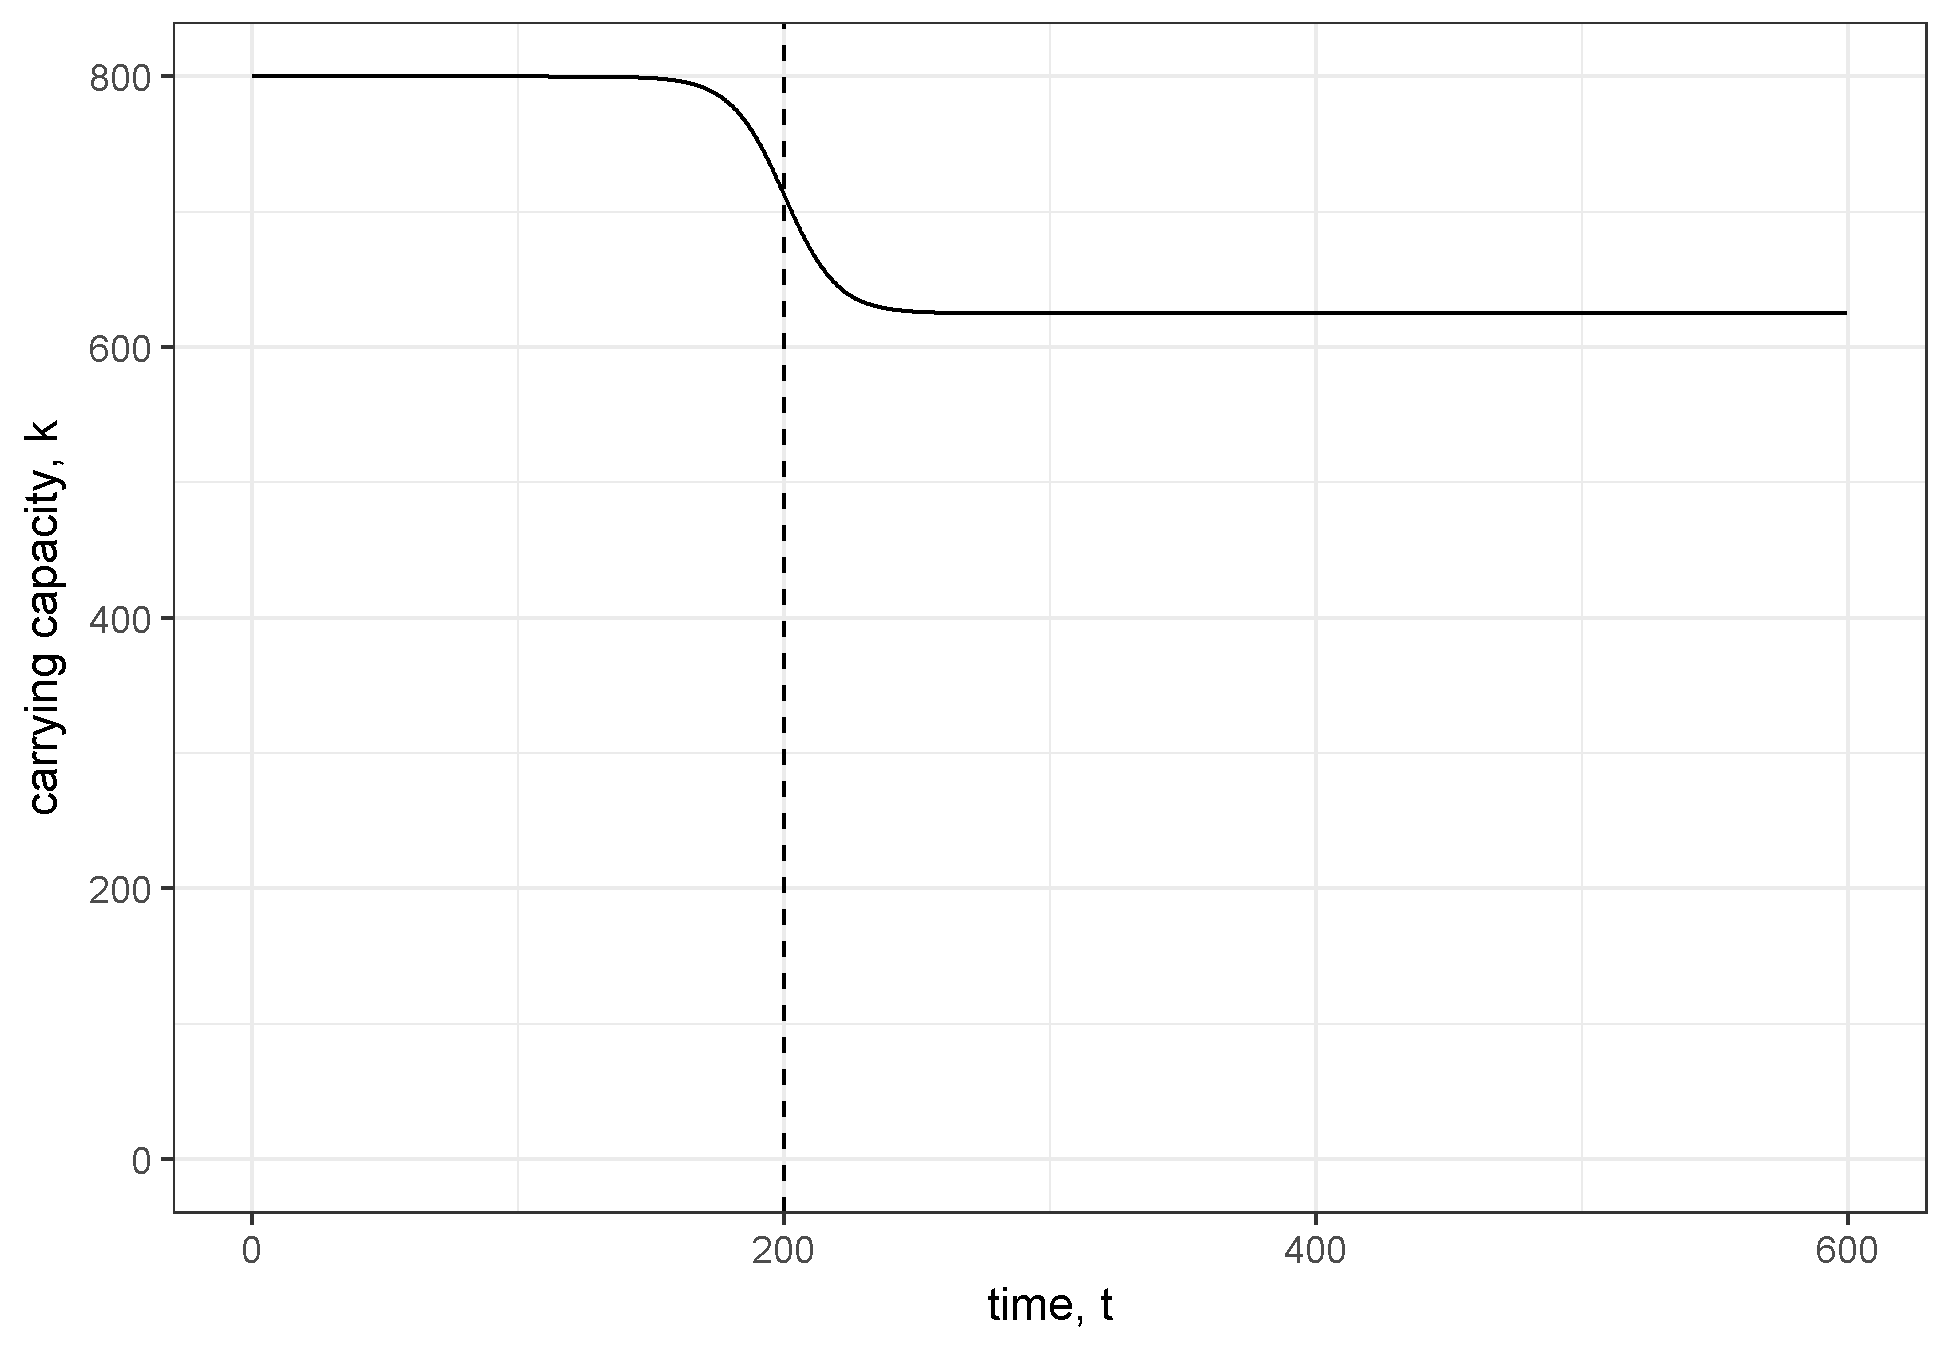
\includegraphics[width=27.08in]{./chapterFiles/fiGuide/figures/kByTime} \caption{Carrying capacity over time with a regime shift occuring around time 200.}\label{fig:kByTime}
\end{figure}
\begin{Shaded}
\begin{Highlighting}[]
\CommentTok{# Plot trajectories}
\KeywordTok{ggplot}\NormalTok{(}\DataTypeTok{data =}\NormalTok{ results_kstudy, }\KeywordTok{aes}\NormalTok{(}\DataTypeTok{x =}\NormalTok{ x1, }\DataTypeTok{y =}\NormalTok{ x2, }\DataTypeTok{color =}\NormalTok{ k)) }\OperatorTok{+}
\StringTok{  }\KeywordTok{geom_path}\NormalTok{() }\OperatorTok{+}
\StringTok{  }\KeywordTok{labs}\NormalTok{(}\DataTypeTok{x =} \StringTok{"prey, x1"}\NormalTok{, }\DataTypeTok{y =} \StringTok{"predator, x2"}\NormalTok{) }\OperatorTok{+}
\StringTok{  }\KeywordTok{coord_fixed}\NormalTok{()}
\end{Highlighting}
\end{Shaded}
\begin{figure}
\centering
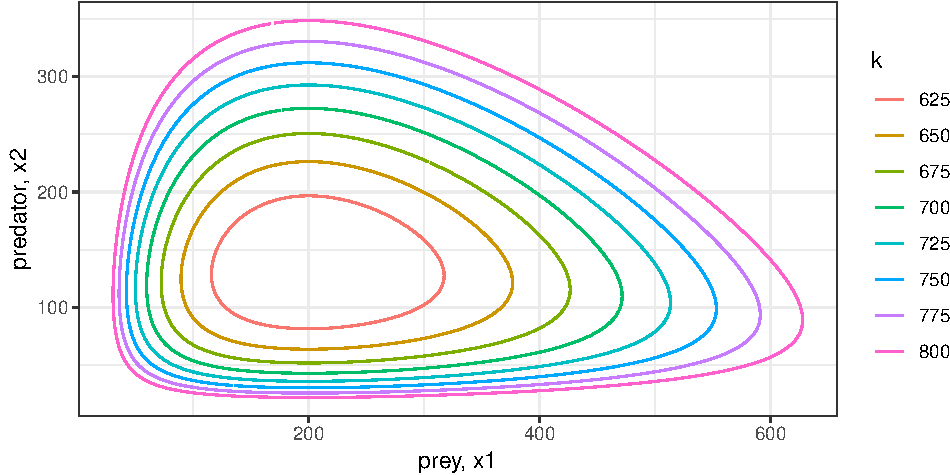
\includegraphics{_myDissertation_files/figure-latex/kTrajectories-1.pdf}
\caption{\label{fig:kTrajectories}Phase space plot of system trajectories
for different values of k}
\end{figure}
We assumed an initial carrying capacity of 800 and a final carrying
capacity of 625 which corresponds to the range of carrying capacities
explored by Mayer et al. (2007). We simulated a time series of 600 time
units with a regime change after 200 time units. We used an alpha value
of 0.05. The time series for carrying capacity is shown in
\ref{fig:kByTime} and the system trajectory in phase space is shown in
\ref{fig:kTrajectories}. The distance travelled in phase space (i.e.,
cumulative change in state) is shown in \ref{fig:distOverTime} and the
speed of the system (i.e., rate of change) is shown in
\ref{fig:dsdtOverTime}.
\begin{Shaded}
\begin{Highlighting}[]
\NormalTok{knitr}\OperatorTok{::}\KeywordTok{include_graphics}\NormalTok{(}\StringTok{'./chapterFiles/fiGuide/figures/dsdtOverTime.png'}\NormalTok{)}
\end{Highlighting}
\end{Shaded}
\begin{figure}
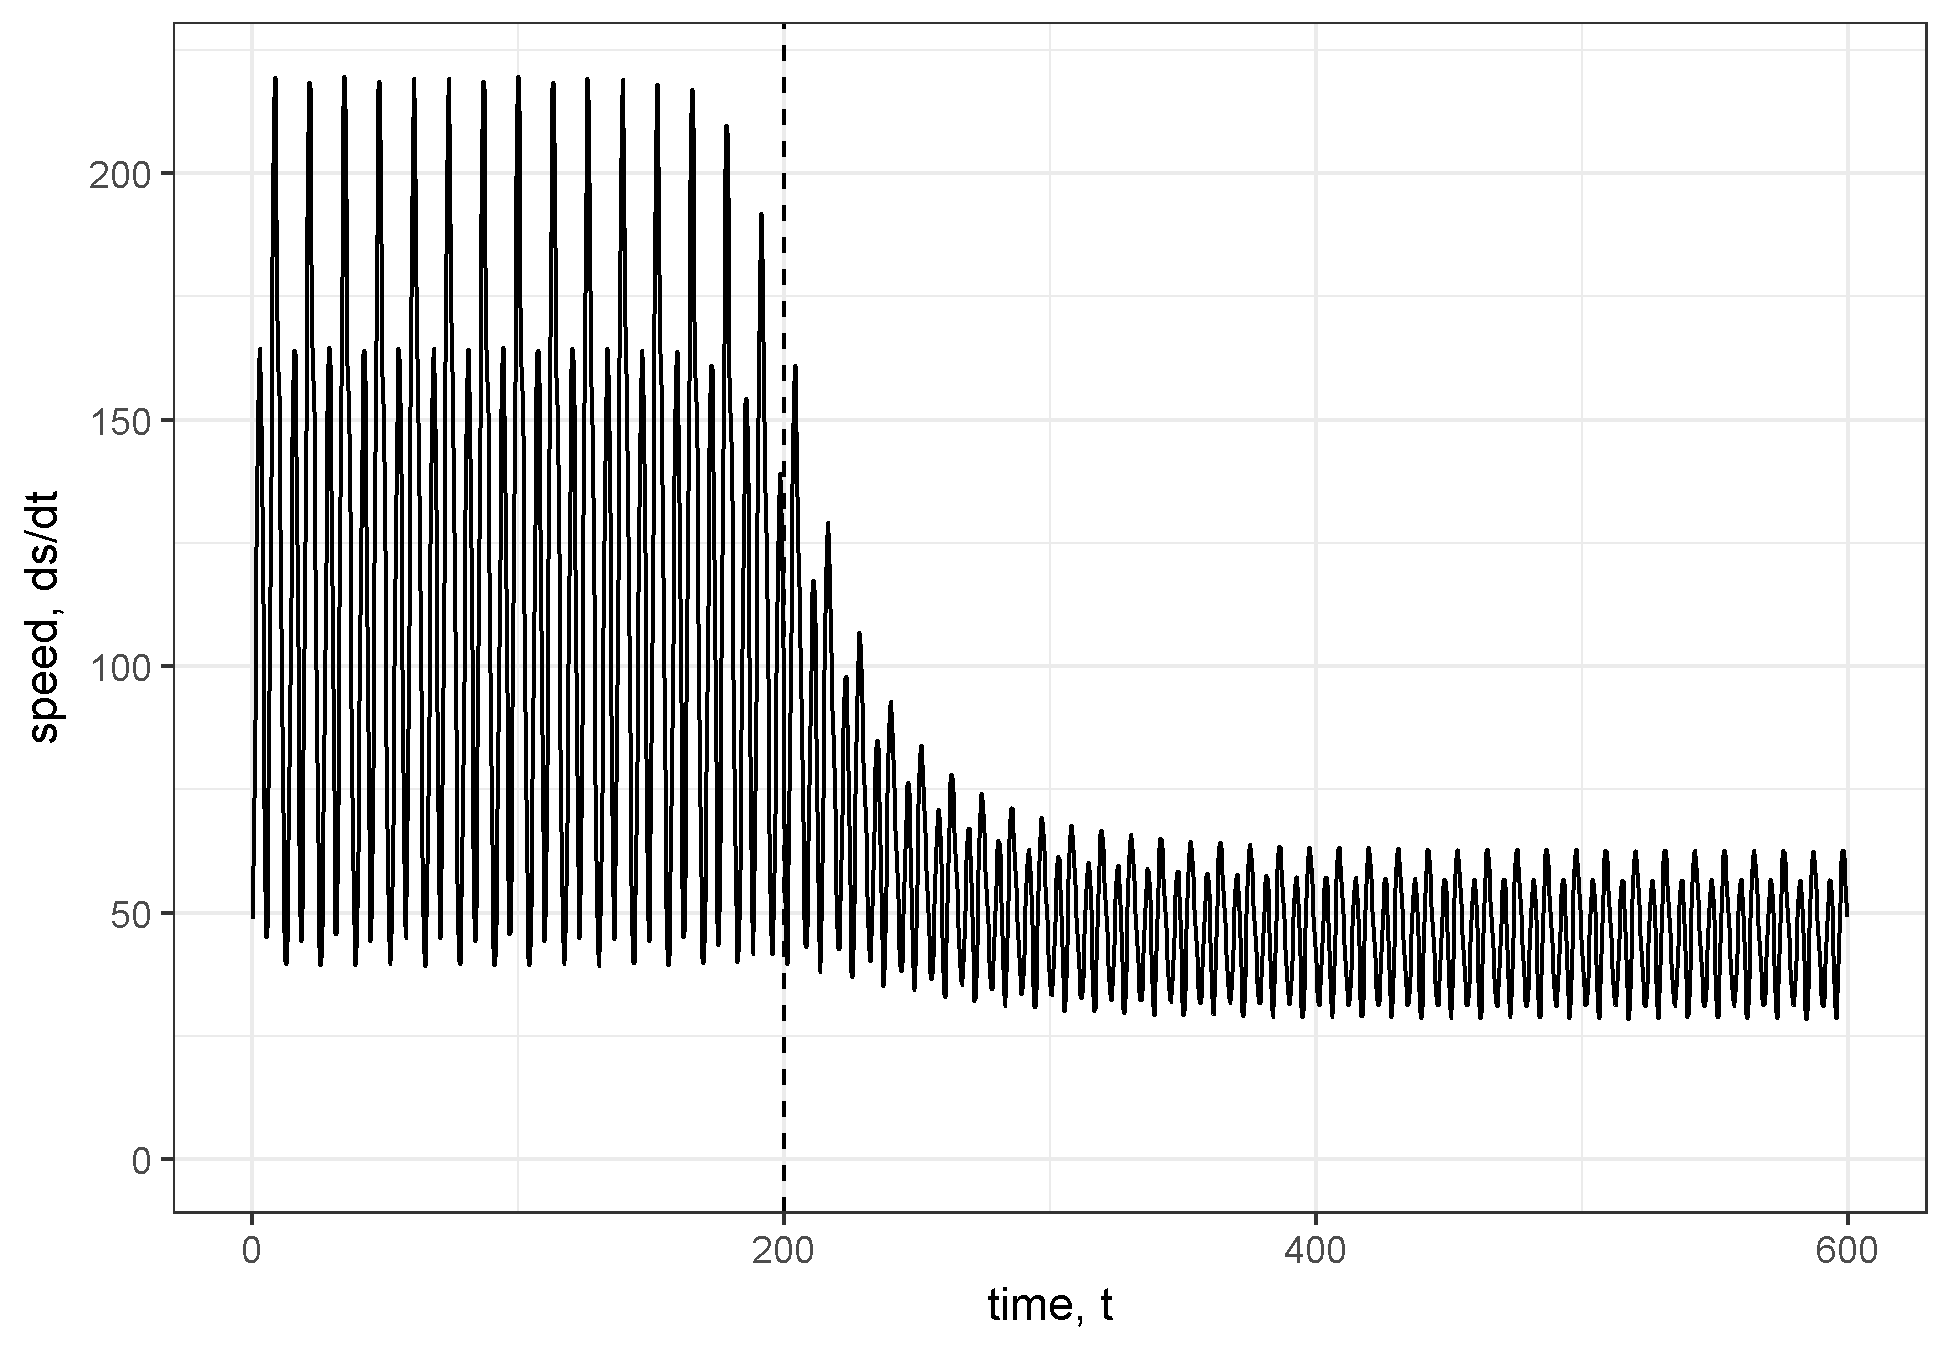
\includegraphics[width=27.08in]{./chapterFiles/fiGuide/figures/dsdtOverTime} \caption{Speed of the system (rate of change) in phase space. Dashed vertical line at time 200 indicates location of regime shift.}\label{fig:dsdtOverTime}
\end{figure}
We calculated FI for the distribution of distance travelled over a
series of non-overlapping time windows. Multiple sources suggest the
length of the time window should be equal to one system period such that
FI is constant for a periodic system (Cabezas \& Fath, 2002; D. A. L.
Mayer et al., 2007). However, the system period is different before,
during, and after the regime shift. Therefore, we performed two separate
calculations of FI using window sizes corresponding to the initial and
final period of the system (\(13.061\) and \(11.135\), respectively).
The change in FI over time is shown in \ref{fig:fiOverTime}.
\begin{Shaded}
\begin{Highlighting}[]
\NormalTok{knitr}\OperatorTok{::}\KeywordTok{include_graphics}\NormalTok{(}\StringTok{'./chapterFiles/fiGuide/figures/fiOverTime.png'}\NormalTok{)}
\end{Highlighting}
\end{Shaded}
\begin{figure}
\includegraphics[width=27.08in]{./chapterFiles/fiGuide/figures/fiOverTime} \caption{Fisher Information calculated for non-overlapping time windows. Two different window sizes were used as indicated by color. Dashed vertical line at time 200 indicates approximate location of regime shift.}\label{fig:fiOverTime}
\end{figure}
\section{Conclusions}\label{conclusions-1}

We simulated a regime shift caused by a change in carrying capacity
(\(K\)) within a simulated, two-species Lotka-Volterra system. We
applied the Fisher Information (FI) method for regime shift detection to
the simulated time series data. The predator-prey system was modeled as
deterministic and the time series data was free from measurement and
observation error. Despite this, the estimated FI had high variation
over time, and results were dependent on the size of the time window
used (winsize) in the calculation \ref{fig:fiOverTime}. The FI method
for regime shift detection is based on the cumulative change in the
state of the system (i.e., distance traveled in phase space) and the
rate of change of the system (i.e., speed tangential to trajectory in
phase space). The distance travelled metric, \(s\), and its speed,
\(dsdt\), appear better visual indicators of the regime shift than FI
{[}\ref{fig:distOverTime}; \ref{fig:dsdtOverTime}{]}.

In our explanation of the FI concept and calculation, we emphasize the
distinction between the \emph{state of the system} and the
\emph{distance traveled in phase space}. There are several reasons worth
emphasizing this. First, there may not always be a one-to-one
relationship between the probability of observing a system in a
particular state and the probability of observing a system at a
particular distance along the trajectory. In these situations the
interpretation of FI may be less clear than if a one-to-one relationship
existed. Second, this distinction facilitates the separation of the
dimensionality reduction step (calculating distance traveled in phase
space, \(s\)) from the subsequent steps related specifically to FI.
Third, the distinction suggests that the \textbf{value of FI as a regime
shift detection method is related to the rate of change of the system}
(i.e., velocity and acceleration tangential to system trajectory in
phase space). In particular, the distribution for which FI is calculated
is simply the distribution of the distance traveled in phase space, when
time is assumed to be uniformly distributed over a given interval.

Our results suggest that insights can be gained directly from the
calculation of distance traveled and associated rates of change.
Consequently, these insights preclude the need to calculate beyond Step
3 (described above). This result also supports the use of the distance
travelled metric, or the derivatives-based Fisher Information
\label{eq:fiDerivs}.

One remaining issue that is prevalent across ecological field studies is
the assumption that the system is observed without error. Although
ecological data rarely fulfill this assumption, this does not suggest
that FI is useless as a metric of system stability. The primary
difficulty with noisy data, especially with observations in integer form
(e.g.~count data), is that the denominator in can easily be zero for
some pair of observations, making FI an infinite value within windows
which contain two or more adjacent zero observations. One possible
solution is to smooth the multidimensional vector of observations prior
to calculating the derivatives, or to treat any sequential identical
value as missing, and simply use a larger time step for that portion of
the window calculation.

The utility of Fisher Information in ecological studies is also stunted
by its interpretability. This metric is unitless, making its values
relative only within-sample (e.g., within a single time series).
Further, interpreting the results within-sample is currently a
qualitative effort (B. D. Fath et al., 2003; Mantua, 2004). When the FI
of a system is increasing, the system is said to be moving toward a more
orderly state, and most presentations of FI posit sharp changes in FI,
regardless of the directionality of the change, may indicate a regime
shift (Cabezas \& Fath, 2002; Karunanithi et al., 2008; T. L. Spanbauer
et al., 2014). Due to the qualitative nature of these interpretations of
Fisher Information, intimate knowledge of the system in question and the
potential driver(s) of the observed regime shift are required to confirm
presence of a shift.

\section{Acknowledgements}\label{acknowledgements}

I thank T. Eason, H. Cabezas and B. Roy Frieden for early discussions
regarding Fisher Information.

\chapter{An application of Fisher Information to spatially-explicit
avian community data}\label{fisherSpatial}
\begin{Shaded}
\begin{Highlighting}[]
\NormalTok{## Only run this if you need to calculate more metrics, or fix them.}
\CommentTok{# source('/chapterFiles/fisherSpatial/04-chap-binning_analysis.R')}
\NormalTok{figDir <-}\StringTok{ "./chapterFiles/fisherSpatial/figures"}
\NormalTok{figDissDir <-}\StringTok{ "./chapterFiles/fisherSpatial/figures/figsCalledInDiss"}
\end{Highlighting}
\end{Shaded}
\section{Introduction}\label{introduction-2}

Ecosystems are open, dynamical systems which arguably cannot be fully
represented by deterministic models. Despite the complexity of most
ecological systems, some patterns have emerged in certain statistical
representations. An uptick in recent years of studies of \textbf{regime
shifts}\footnote{see \ref{glossary} for a definition} in ecology
{[}\ref{wosRegimePubsByYear}{]} has spurred an increase in the number of
`new' methods for detecting ecological regime shifts
{[}\ref{rdmReview}{]}, some of which are proposed as indicators of
`spatial' regime shifts (Butitta, Carpenter, Loken, Pace, \& Stanley,
2017, Kefi et al. (2014), Sundstrom et al. (2017b), ({\textbf{???}}), W.
Brock \& Carpenter (2006)).

As defined in \ref{Glossary}, a regime shift is largely considered an
abrupt and persistent change in a system's structure or functioning.
Following this definition and without any associated \textbf{pressures}
\ref{Glossary}, it is not yet clear whether identifying a `spatial
regime' using a snapshot of a system (a single or short period of time
relative to the time scale of the pressure) is pragmatic. One spatial
regime detection measure (hereafter, SRDM) is variance (W. Brock \&
Carpenter, 2006), despite its controversial applicability to temporal
data ({\textbf{???}}, Dutta et al. (2018), Charles T Perretti \& Munch
(2012), ({\textbf{???}}), Bestelmeyer et al. (2011)).

Defining the spatial regime shift is important since observations of
non-random spatial processes (e.g., land cover), could manifest as
either rapid shift (e.g.~an ecotone) or a gradual change (slow mixing
along a gradient). Consequently, and because most RDMs signal abrupt
change, only the former may be identified as ``regime shifts'' using
SRDMs. For the concept of spatial regimes to be ecologically useful,
potential pressures must be associated with system structure over space
\emph{and} time. Additionally and perhaps more importantly, the
processes driving the observed information (drivers, pressures ) should
be such that a statistically identified regime shift will roughly
correspond with the time scale on which the pressure(s) operate.

Although it is suggested that statistical and pragmatic models and
methods are advanced more rapidly by bottom-up approaches, i.e.~case
studies (see DeAngelis \& Yurek, 2017), to my knowledge no studies have
yet to test the rigor of SRDMs using spatially-explicit empirical data.
The objective of this chapter is to determine the utility of Fisher
Information (Eq. \eqref{eq:fiDerivs}) as a spatial regime detection
measure. This chapter is also supported by original software developed
for implementation in Program R, which is publicly available
{[}\ref{burnett2019regime}{]}.

\section{Methods}\label{methods-1}

\subsection{Data: North American Breeding Bird
Survey}\label{data-north-american-breeding-bird-survey}

I use community abundance data from long-term monitoring programs to
identify spatial and temporal regimes using the Fisher Information (FI)
derivatives method (see Eq. \ref{derivatives}). The NABBS trains citizen
scientist volunteers to annually collect data using a standardized
roadside, single observer point count protocol and has been collecting
data regularly across North America (\ref{fig:bbsPoints}) since 1966.
The roadside surveys consist of 50 point counts (by sight and sound)
along an approximately 24.5 mile stretch of road. Due to strict reliane
on volunteers, some routes are not covered every year. Additionally,
some routes are moved or discontinued, and some routes are not sampled
in a given year. Route-year combinations which are missing years but are
not discontinued are treated as missing data. Although NABBS volunteers
identify all species as possible, persistent biases exist in this
protocol. To reduce the influence of potential sampling bias, I removed
waterfowl, waders, and shore species (AOU species codes 0000 through
2880).
\begin{Shaded}
\begin{Highlighting}[]
\NormalTok{knitr}\OperatorTok{::}\KeywordTok{include_graphics}\NormalTok{(}\KeywordTok{paste0}\NormalTok{(figDissDir, }\StringTok{"/bbsRoutesUsed.png"}\NormalTok{))}
\end{Highlighting}
\end{Shaded}
\begin{figure}
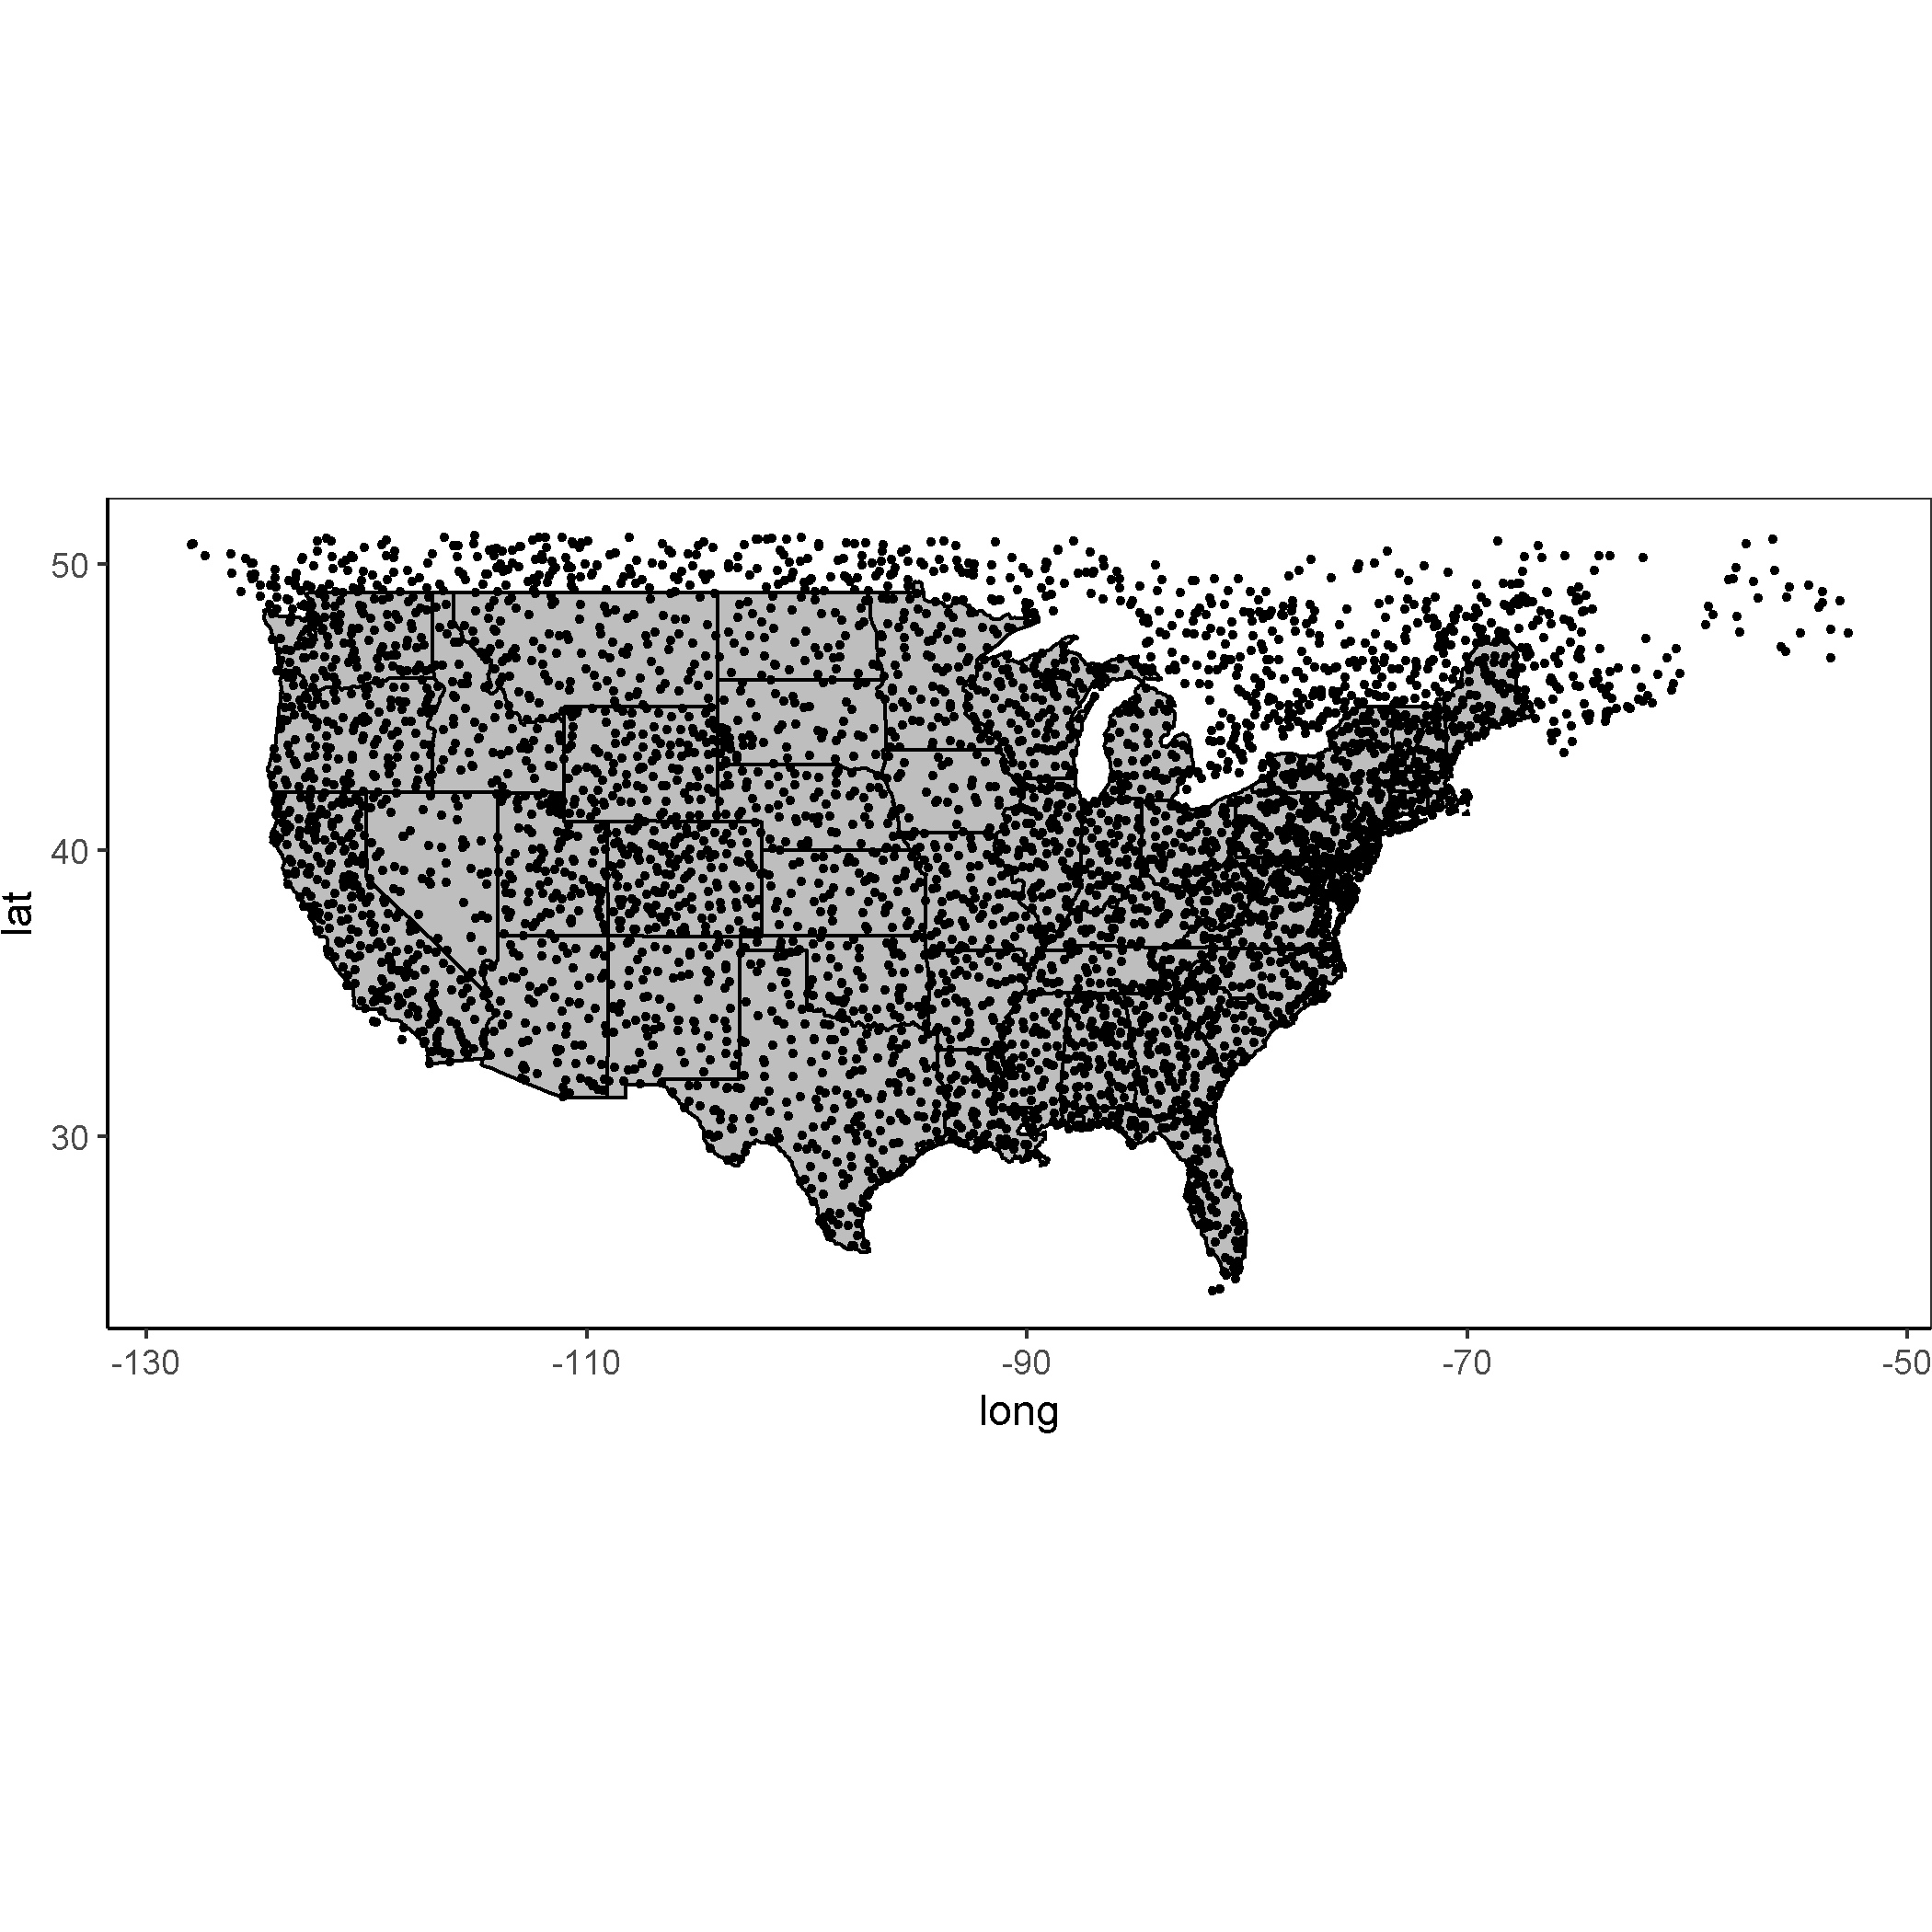
\includegraphics[width=30.03in]{./chapterFiles/fisherSpatial/figures/figsCalledInDiss/bbsRoutesUsed} \caption{Locations of Breeding Bird Survey routes sampled between 1966 and 2017.}\label{fig:bbsPoints}
\end{figure}
\subsection{Study areas}\label{study-areas}

Although the NABBS conducts surveys throughout much of North America, I
limited analyses to the continental United States and parts of southern
Canada. NABBS coverage of the boreal forests of Canada are sparse in
space, and many routes in Mexico have fewer than 25 years of
observations. I identified two strip-transects across large swaths of
the continental United States-one running in a South-North direction,
the other running East-West-and two individual NABBS sites (routes) to
conduct spatial and temporal regime shift analyses, respectively. The
South-North and East-West transects are hereafter referred to as spatial
transects, and the NABBS sampling sites are referred to as routes (see
section `Building spatial transects', below).
\begin{figure}

{\centering 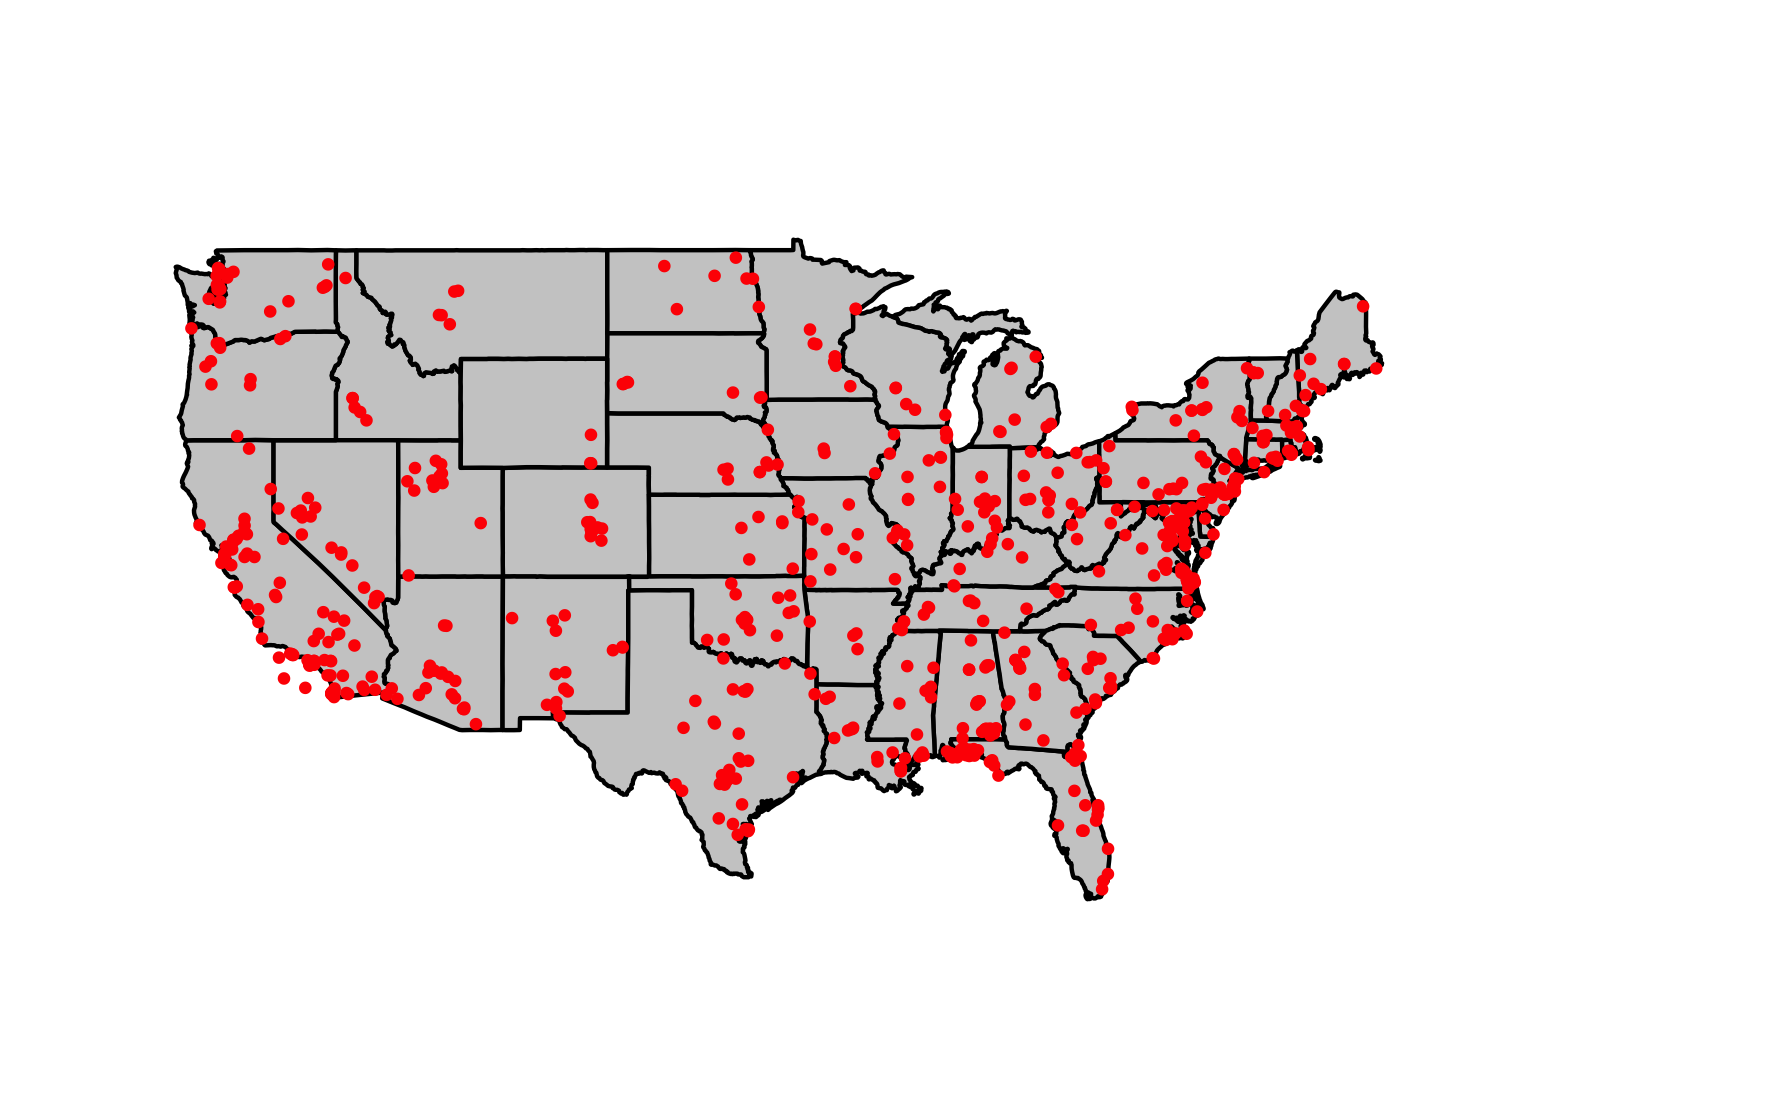
\includegraphics[width=30.03in]{./chapterFiles/fisherSpatial/figures/figsCalledInDiss/milBases} 

}

\caption{Locations of U.S. military bases in our study area.}\label{fig:milBases}
\end{figure}
\subsubsection{Military bases as study
sites}\label{military-bases-as-study-sites}

The Mission of the US Department of Defense is to provide military
forces to deter war and protect the security of the country, and a
primary objective of individual military bases is to maintain military
readiness. To maintain readiness, military bases strictly monitor and
manage their natural resources. Military bases vary in size and nature,
and are heterogeneously distributed across the continental United States
(See \ref{fig:ewRouteMap}). The spread of these bases
(\ref{fig:milBases}), coupled with the top-down management of base-level
natural resources presumably influences the inherent difficulties
associated with collaborative management within and across military
bases and other natural resource management groups (e.g., state
management agencies, non-profit environmental groups.

Much like other actively managed landscapes, miltiary bases are
typically surrounded by non- or improperly-managed lands. Natural
resource managers of military bases face environmental pressures within
and surrounding their properties, yet their primary objectives are very
different. Natural resource managers of military bases, whose primary
objective is to maintain military readiness, are especially concerned
with if and how broad-scale external forcings might influence their
lands. Prominent concerns include invasive species, wildlife disease,
and federally protected species (personal communication with Department
of Defense natural resource managers at Eglin Air Force and Fort Riley
military bases). For these reasons, natural resource managers attempt to
create buffers along their perimeters (e.g., live fire/ammunitions
suppression, wide fire breaks). Identifying the proximity of military
bases to historic and modern ecological shifts may provide insight into
the effectiveness of their natural resource management efforts.

\subsubsection{Focal military bases}\label{focal-military-bases}

The NABBS routes chosen for analyses in this Chapter lie within or near
two two US Department of Defense properties: Fort Riley military base
(located at approximately \(39.110474^{\circ}\), \(-96.809677^{\circ}\);
Kansas, USA) and Eglin Air Force base (located at approximately
\(30.459588^{\circ}\), \(-86.548459^{\circ}\); Florida USA). These
military bases were used for research conducted under the a grant funded
by the Department of Defense's Strategic Environmental Research and
Development Program (SERDP; RSCON-15-01:RC 3150).

Eglin Air Force and Fort Riley military bases
(\ref{fig:basesOfInterestMap}) serve as ideal reference sites for this
study. The natural resource management teams are active on each base and
have been for at least two decades and each uses wildfire as a
management technique. Fort Riley military base is especially relevant to
regime shift detection method exploratory analysis. Woody encroachment
of the Central Great Plains over the last century has triggered shifts
in dominant vegetative cover and diversity (Ratajczak et al. 2012) in
the area surrounding Fort Riley military base (e.g., Van Auken 2009).
This phenomena should present itself as a regime boundary should Fisher
Information be a robust regime shift detection method. Eglin Air Force
base is embedded within a heavily developed matrix, and consequently has
experienced less pronounced effects at broad spatial extent and over
longer periods. Therefore, the ecological communities (and the data)
surrounding Eglin Air Force base may exhibit a greater amount of noise,
making the effect size of a regime shift and consequently the effect
size smaller and more difficult to detect. For these reasons, Eglin Air
Force and Fort Riley military bases are ideal locations for an
exploratory analysis of the Fisher Information as an SRDM.
\begin{figure}

{\centering 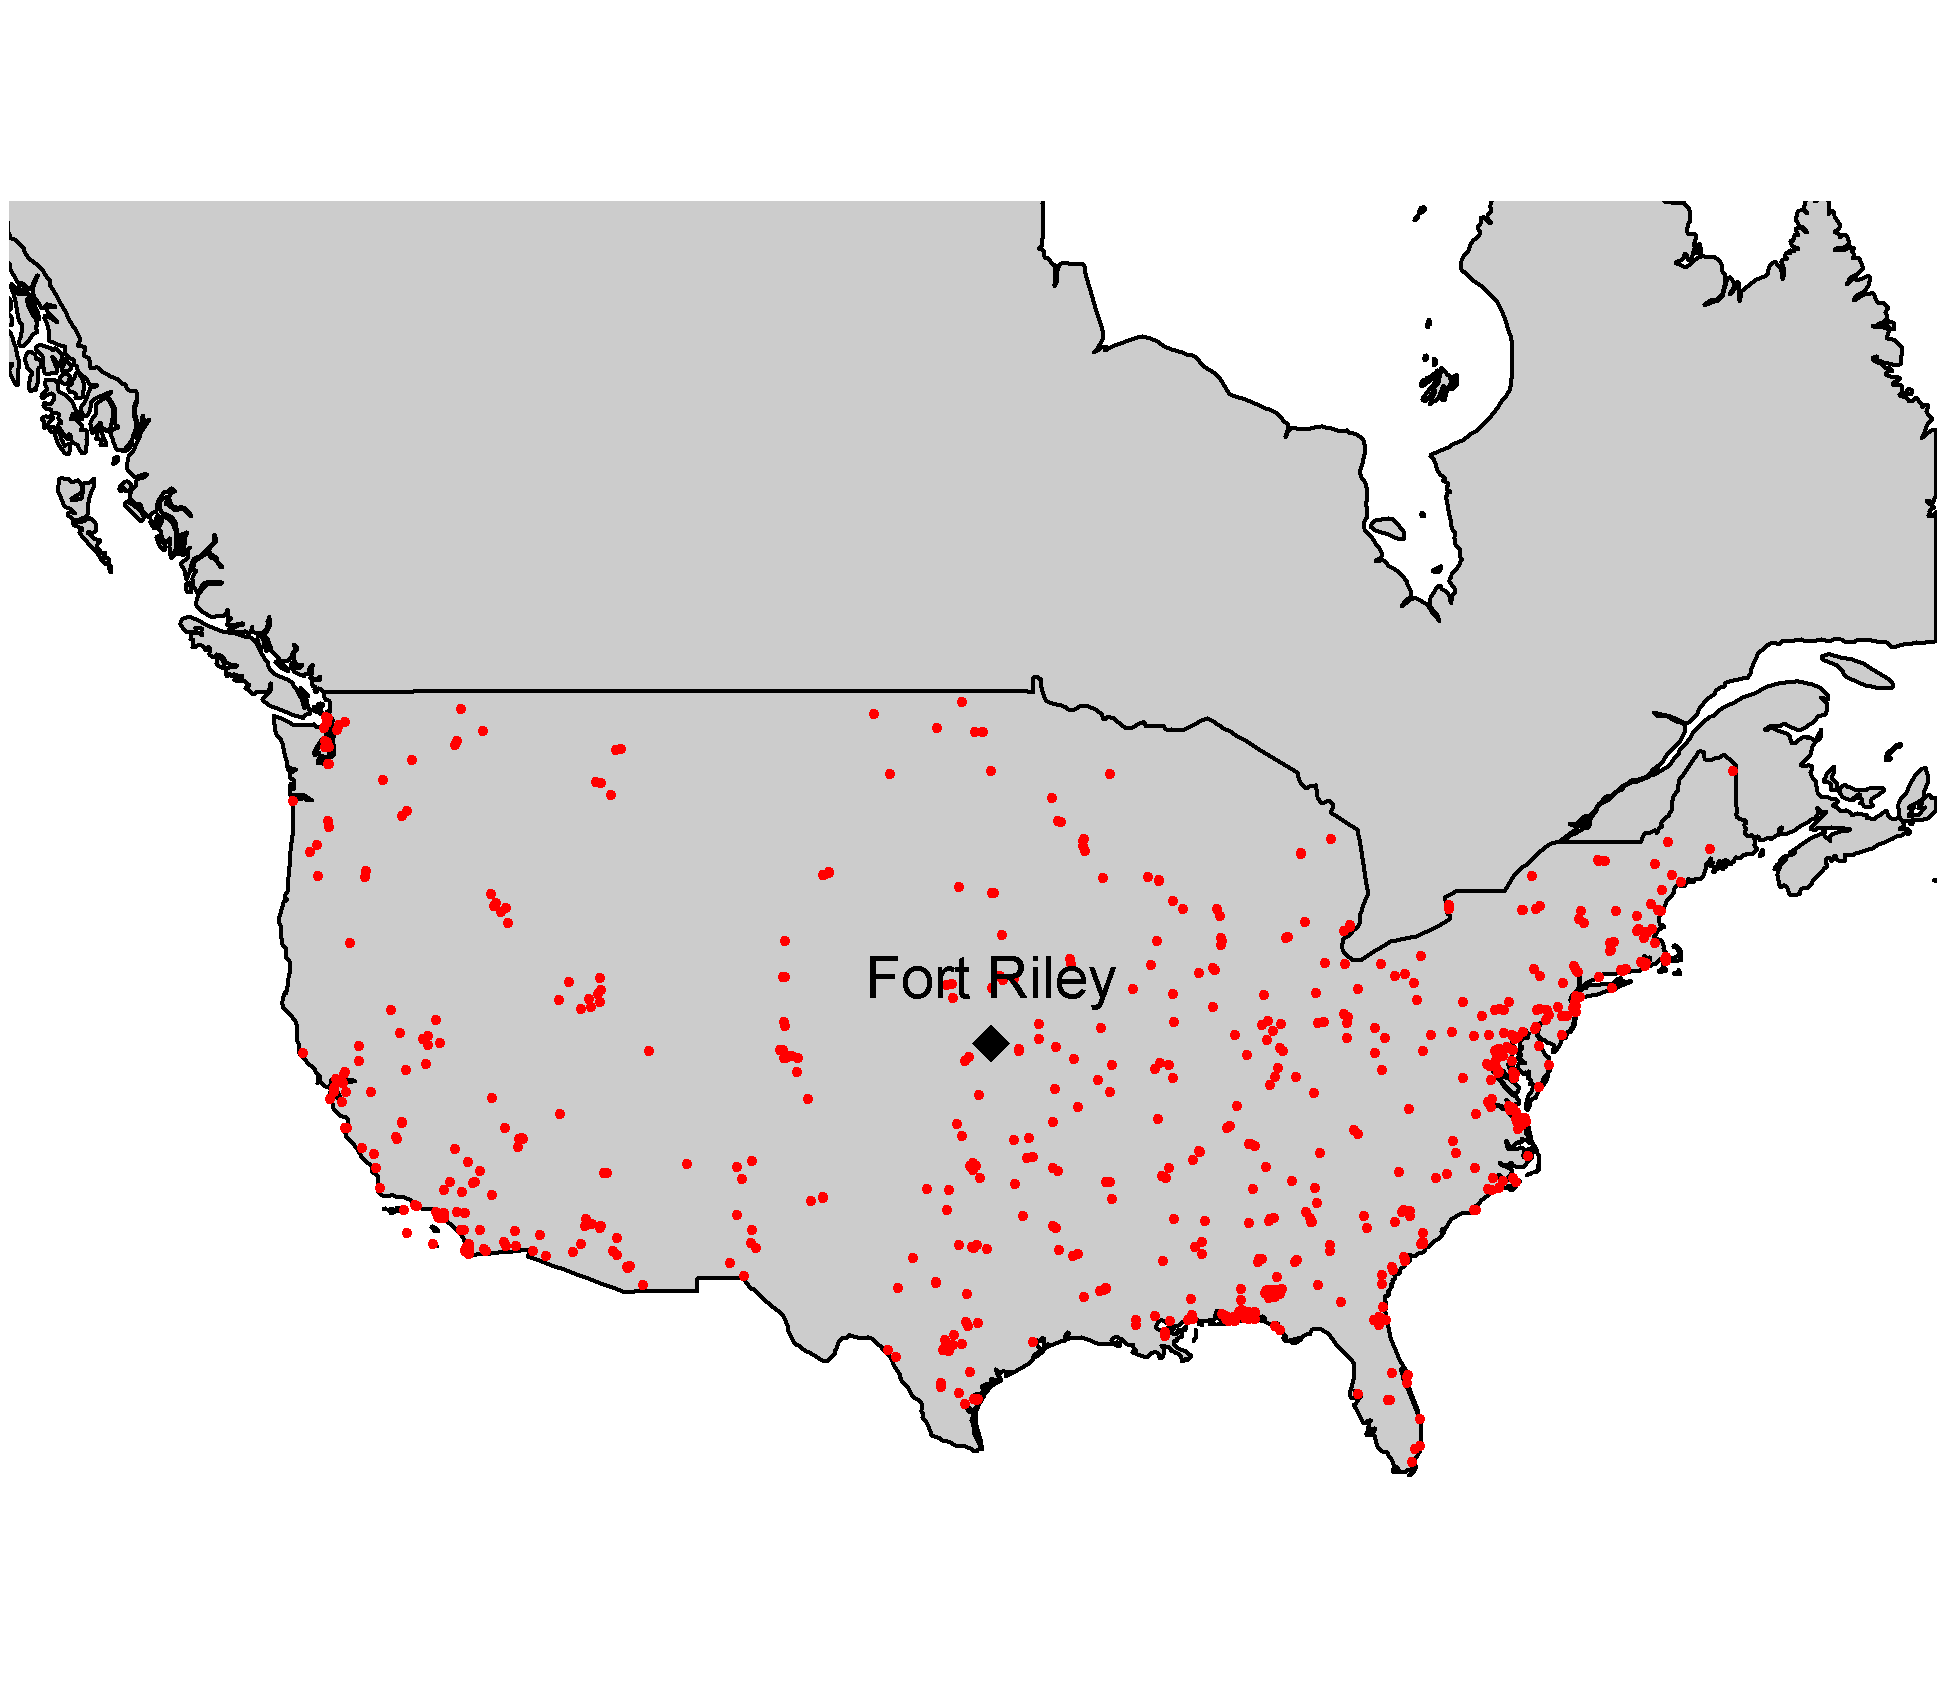
\includegraphics[width=30.03in]{./chapterFiles/fisherSpatial/figures/figsCalledInDiss/basesOfInterestMap} 

}

\caption{Locations of focal U.S. military bases, Eglin Air Force Base (AFB) and Fort Riley Military Base.}\label{fig:basesOfInterestMap}
\end{figure}
\subsubsection{Spatial sampling grid}\label{spatial-sampling-grid}

To my knowledge, Sundstrom et al. (2017a) is the only study to use the
Fisher Information binning method on spatially-referenced data. The
authors of this study hand-picked NABBS routes to be included in their
samples such that their metrics should detect `regime changes' when
adjacent sampling points represented different ecoregions (broad-scale
vegetation classification system). The authors also suggest each
ecoregion is similarly represented, having a similar number of NABBS
routes within each ecoregion in the analysis. However, this method of
handpicking routes resulted in a transect which was neither North-South
nor East-West running (see Sundstrom et al. (2017a)), but rather
zigzagged across a midwestern region.

I constructed a gridded system across much of the continental United
States and Canada to ameliorate potential effects of site selection
bias. This method allows one to overlay regime detection metric results
over various vegetation characteristic maps (e.g., ecoregions), rather
than fit the sampling scheme to an ecoregion. The former also allows for
comparison of results across time, and is especially useful when
vegetation zones, or ecoregions, shift over time.

The gridded system comprises North-South and East-West running transects
transects running in either North-South or East-West directions. Here, I
examine in detail only a single North-South and a single East-West
transect, such that they contain the Eglin Air force and Fort Riley
military bases, respectively.
\begin{figure}

{\centering 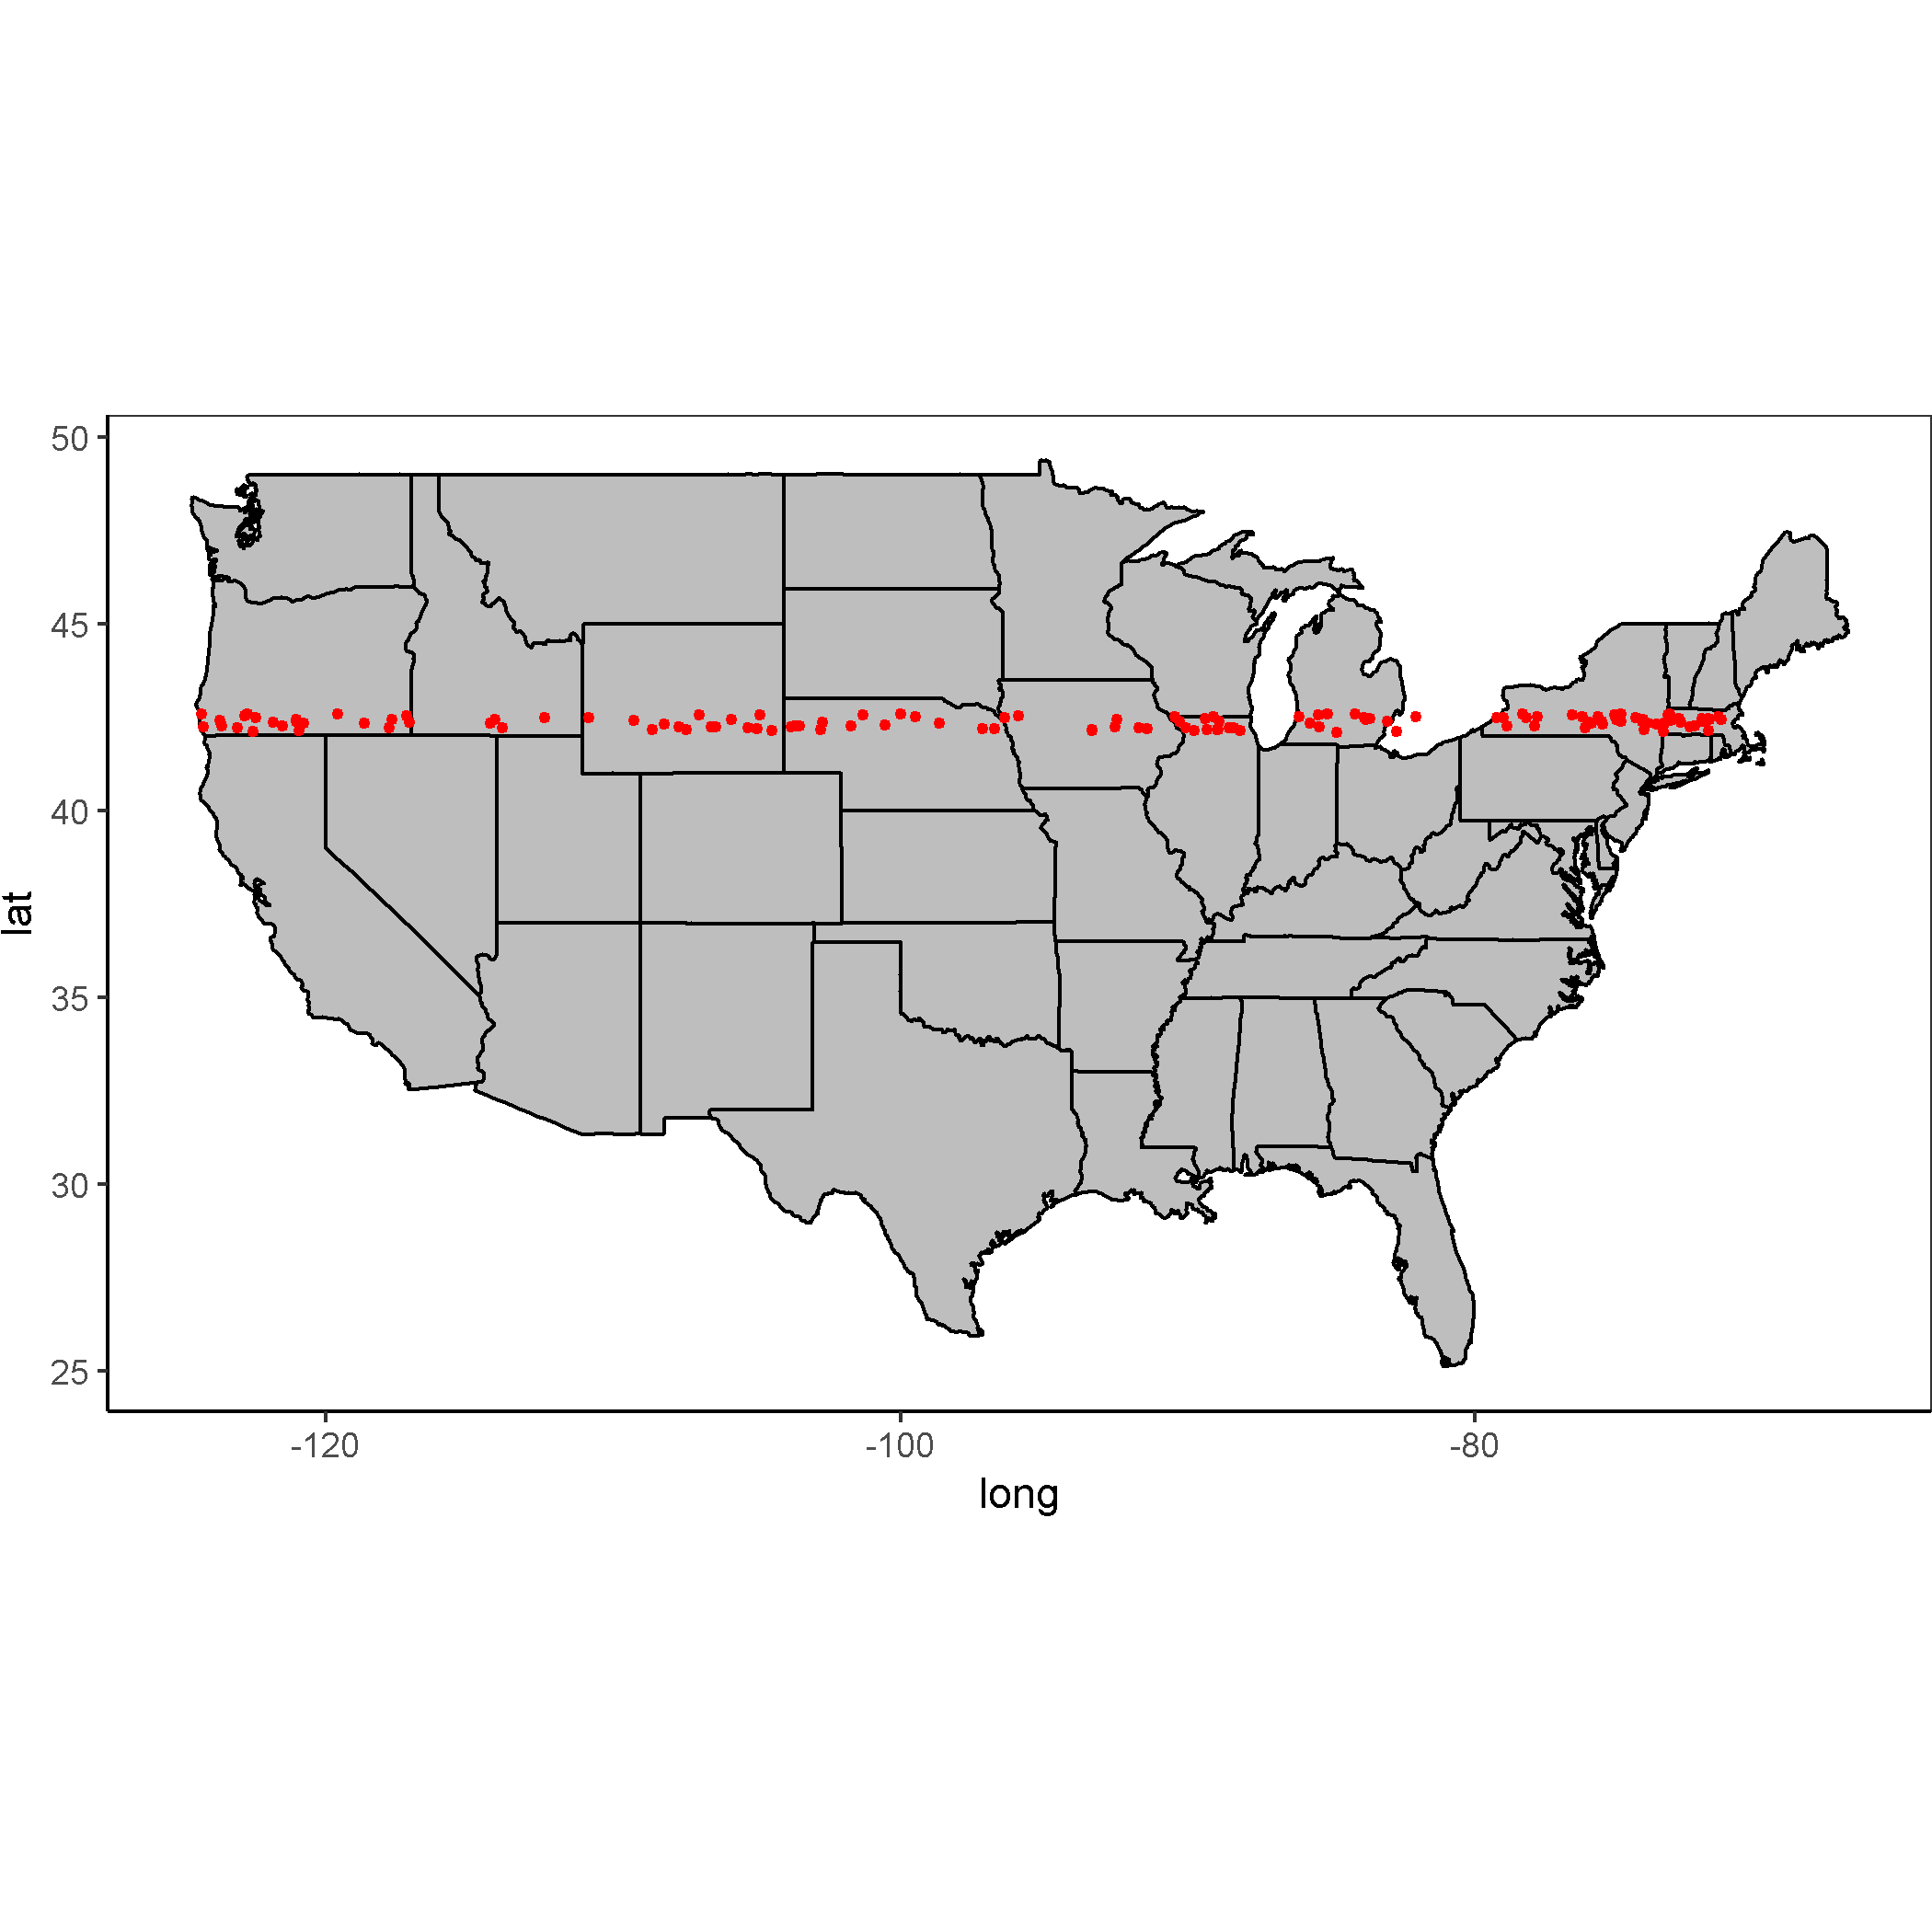
\includegraphics[width=30.03in]{./chapterFiles/fisherSpatial/figures/figsCalledInDiss/transectSamplingEx_row18} 

}

\caption{A single East-West transect of Breeding Bird Survey routes used to calculate the Fisher Information binning measure. Military base locations can be used to visually estimate the proximity [of Department of Defense properties] to potential regime boundaries.}\label{fig:ewRouteMap}
\end{figure}
\subsubsection{Selecting routes for temporal
analysis}\label{selecting-routes-for-temporal-analysis}

Temporal analysis consisted of time series of annually collected data at
the level of an individual NABBS route. I analyzed two NABBS routes near
the Eglin Air Force base-one to the East and one to the West.

\subsection{Calculating regime detection
measures}\label{calculating-regime-detection-measures}

Fisher Information, \(I(\theta)\), was developed in 1922 by Ronald
Fisher as a measure of the amount of information that an observable
variable, X, reveals about an unknown parameter, \(\theta\). Fisher
Information is a measure of indeterminacy (Fisher 1922) and is defined
as,
\begin{equation} 
I(\theta) = \int \frac{dy}{p(y|\theta)}\left[\frac{dp(y|\theta)}{d\theta}\right]^2
\label{eq:fiGeneral1922}
\end{equation}
where \(p(y|\theta)\) is the probability density of obtaining the data
in presence of \(\theta\). The Fisher Information measure (FIM) is used
to calculate the covariance matrix associated with the likelihood,
\(p(y|\theta)\). Fisher Information is described as Extreme Physical
Information (EPI; Frieden and Soffer 1995, Kibble 1999, Frieden et al.
2002), a measure that has been used to track the complexity of systems
in many scientific disciplines including, physics, cancer research,
electrical engineering, and, recently, complex systems theory and
ecology

Fisher Information as gathered from observational data provides insight
as to the dynamic order of a system, where an orderly system is one with
constant (i.e., unchanging) observation points, and one whose nature is
highly predictable. A disorderly system is just the opposite, where each
next data point is statistically unpredictable. In ecological systems,
patterns are assumed to be a realization of ecosystem order; therefore,
oneshould expect orderliness in a system with relatively stable
processes and feedbacks. Orderliness, however, does not necessarily
infer long-term predictability. \eqref{eq:fiGeneral1922} is next adapted
to estimate the dynamic order of an entire system, \(s\), as
\begin{equation} 
I = \int \frac{ds}{p(s)}\left[\frac{dp(s)}{ds}\right]^2
\end{equation}
where \(p(s)\) is the probability density for \(s\). Here, a relatively
high Fisher Information value (\(I\)) infers higher dynamic order,
whereas a lower value (approaching zero) infers less orderliness. To
limit the potential values of \(I\) in real data, we can calculate the
amount of Fisher Information by re-expressing it in terms of a
probability amplitude function \(q(s)\) (Fath et al. 2003, Mayer et al.
2007, eq. 7.3):
\begin{equation}
I = 4 \int ds\left[\frac{dq(s)}{ds}\right]^2
\end{equation}
A form specific to the pdf of distance travelled by the entire system,
which I call the `derivatives' method, is defined as (D. A. L. Mayer et
al., 2007, eq. 7.12):
\begin{equation}
I = \frac{1}{T} \int_0^T dt\left[\frac{s''^2}{s'^4}\right]^2
\end{equation}
, where T is the number of equally spaced time points over which the
data are integrated. Numerical calculation of \(I\) using the binning
method (Eq. \eqref{eq:fiAmplitude} and \eqref{eq:derivativesFI}) each
incorporate a moving-window procedure for calculating the probability of
the system, \(p(s)\), as being in one of an unidentified number of
states (\(s\)). Although previously applied to spatially-explicit
terrestrial community data,the binning method (Eq. \ref{derivatives})
requires multiple parameters to be defined \emph{a priori}, which have
been shown to influence inference based on the metric. I therefore
calculated FI using the derivatives equation (Eq. \ref{fiDerivs}).

The binning procedure allows for a single point in time or space to be
categorized into more than one state, which violating the properties of
alternative stable states theory. The size of states (see Eason and
Cabezas 2012) measure is required to construct p(s). In the case of high
dimensional data, a univariate binning procedure of p(s) is not
intuitive (i.e., reducing a multivariable system to a single probability
distribution rather than constructing a multivariate probability
distribution). Importantly, when using community or abundance data, rare
or highly abundant species can influence the size of states criterion,
thus influencing the assignment of each point into states. Finally, Eq.
\eqref{eq:fiAmplitude} assumes equal spacing (in space or time) between
sampling points. Each of these violations can be avoided by using Eq.
\eqref{eq:derivativesFI}; Cabezas and Fath 2002, Fath et al. 2003) to
calculate the Fisher Information measure (see Chapter @derivatives for
discussion on this topic). The derivatives method (Eq.
\eqref{eq:derivativesFI}) estimates the trajectory of the system's state
by calculating the integral of the ratio of the system's acceleration
and speed in state space (B. D. Fath et al., 2003).

\section{Results}\label{results-1}

\section{Discussion}\label{discussion-1}

Current methods for identifying ecological regime changes in noisy,
complex data are imperfect and require strict assumptions and detailed
knowledge of the system. The Fisher Information binning measure was
introduced to avoid some analytical issues related to complex and noisy
data in the analaysis of ecological data (Karunanithi et al. 2008). This
study found that the Fisher Information binning measure and other
analytical techniques have a long way to go prior to being ready for
ubiquitous application. It is vital for the user to understand the
assumptions of estimating dynamic order and identifying regime changes
in ecological systems using Fisher Information as the feasibility of
calculating I using noisy data is still being explored (Sundstrom et al.
2017). There are three primary assumptions required when using Fisher
Information to estimate relative orderliness within ecological data
(Mayer et al. 2007):\\
1. the order or state(s) (\(s\)) of the system is observable, 1. any
observable change in the information observed in the data represents
reality and the variables used in the analyses will not produce false
negatives, and 1. changes in \(I\) presumed to be regime shifts do not
represent the peaks of cyclic (periodic) patterns.

The first assumption is one of philosophical debate and is thus not
controllable. To attempt to control for false negatives, the user should
take caution in her choice of input variables. In the the case of a very
large, multivariate dataset, relativization and/or variable reduction
measures may be useful (Rodionov 2005). To account for cyclic behavior
in the data, we can take measures to ensure our integration periods
capture at one full cycle of the system (Mayer et al. 2007). Increasing
the integration period may also alleviate some issues of noisiness.

Although the current calculation of Fisher Information for complex
systems is a relatively straightforward process and is mathematically
grounded, care should be taken when applying to ecological data due to
its often sparse and noisy nature. Further, the boundaries of
interpretation of \(I\) for identifying ecological regime shifts are
still under exploration.

Is it possible to identify regiem changes with as many as 25 points
across space, for large regions? The lack of patterns identified using
Fisher Information may also be duet o the fact that (1) tehse data were
designed to identify species trends, not cahnges in communities across
space, (2) even wiht !\textasciitilde{}30 poiunts across space, is this
sufficeint \# of observations to identify regime changes in space? If
this were time, would 30 years, e.g., be enough to observe cahgnes
induced by slow drivers? No.

Using these methods, e.g., Fisher Ifnormation, to identify rapid shfits
in bird communities is not sufficient to suggest a regime shift. In
accordance with Mac Nally et al. (2014), sufficient evidence of a regiem
shift must also include statistical evidence of drivers or pressures.

Even if statistical methods/RDMs suggest that regime shifts have
occurredc across large spatial extents, such as our East-West transect
of avian communities, there is no way to test using a BACI, since the
environmental conditions presumably driving observed changes at large
spatial scales are NOT limited only to our transect.

I think that, due to the short time period of our study
(\textasciitilde{}30 years), we can not suggest regime shifts have
occurred, since anthropogenic influences on environmental conditions
have yet to or have only recently begun. This study can help to provide
baseline measures for what RDM measures look like across space, for our
community, but cannot make inference beyond this.

While the birds in our communities may be self-sustaining, if the
habitat or charactersitics providing opportunity adn resources to these
birds are relics, then the birds will appear as non-self-sustaining.

\section{Unused text}\label{unused-text}

\subsection{Interpreting the Fisher Information binning
method}\label{interpreting-the-fisher-information-binning-method}

Here I define a potential regime change as a point in time or space that
exhibits a relatively large change in the Fisher Information value and
which has a non-zero first derivative. Regime shifts are identified as
data changing from one state to another, thus, rapid shifts in the value
of I should indicate the points, in time or space, at which the system
undergoes reorganization. Spatial and temporal Fisher Information
calculation does not vary, but interpretation of either differ in that a
spatial analysis will identify a spatial regime boundary (Sundstrom et
al. 2017) in space within a single year (or a single aggregation of
years). Analysis of temporal data will identify a point(s) in time at
which a system in a specific location undergoes a regime shift. I follow
the methods outlined in the relevant literature for interpreting the
Fisher Information binning measure (e.g., Karunanithi et al. 2008, Eason
and Cabezas 2012, Sundstrom et al. 2017).

Interpreting the Fisher Information binning measure is currently a
qualitative effort. I interpret an increase in I as increasing system
order (Mantua 2004), and periods of relatively high values of I as the
system occurring in a single state, or fluctuating around a single
attractor. A rapid change in I indicates the system is no longer orderly
and may be undergoing a reorganization phase (Holling 1992). Whether
Fisher Information can identify a switch among basins of attraction
within a single, stable state (or around a single attractor) remains
unknown, as does the number of states which a system can occupy.

When a system occurs within any number of states equally, i.e., p(s) is
equal for each state, both the derivative, (\(\frac{dq(s)}{ds}\), and
\(I\) are zero. As \((\frac{dq(s)}{ds} \rightarrow \infty)\), we infer
the system is approaching a stable state, and as
\(\frac{dq(s)}{ds} \rightarrow 0\) the system is showing no preference
for a single stable state and is on an unpredictable trajectory.
\eqref{eq:fiAmplitude} bounds the potential values of Fisher Information
at \([0, 8]\), whereas \eqref{eq:fiGeneral1922}, \eqref{eq:fi73c}, and
\eqref{eq:derivativesFI} have are positively unbounded \([0, \infty)\). If
the Fisher Information is assumed to represent the probability of the
system being observed in some state, s, then the absolute value of the
Fisher Information binning measure is relative within a single datum
(system). Thus, trends in Fisher Information should be interpreted
relatively, but not absolutely.

Authors of a recent case study of spatial regime shifts
{[}\ref{sunstrom2017detecting}{]} suggest that using the Fisher
Information (binning) method (Eq. \eqref{eq:fiAdapted})

Applications of these quantitative methods to real systems data, coupled
with expert knowledge, are required to advance regime change theory.

\chapter{Distance travelled}\label{distance-chapter}

\chapter{Introduction}\label{introduction-3}

Defining a regime shift

There are different types fo regime shifts, and \textbf{why those
differences matter}
\begin{itemize}
\tightlist
\item
  only ???regime shifts??? that are also ???critical transitions???
  should show ???critical slowing down???
  \begin{itemize}
  \tightlist
  \item
    so that???s an important \emph{technical distinction} if you???re
    trying to use \emph{???early warning signals???}.\\
  \end{itemize}
\item
  There are mutiple types og \textbf{critical transitions}
  \begin{itemize}
  \tightlist
  \item
    these results in very different changes in time series\\
  \item
    in some contexts, this doesn't really matter
  \end{itemize}
\end{itemize}
\chapter{Methodology}\label{methodology}

\chapter{Case study}\label{case-study-1}

\chapter{Discussion}\label{discussion-2}

\appendix

\chapter*{Appendix A}\label{rRDM}
\addcontentsline{toc}{chapter}{Appendix A}

This appendix contains the vignette associated with the R Package,
\texttt{rRDM}. Development source code for this package is available on
GitHub as a compressed file,
\url{https://github.com/TrashBirdEcology/rRDM/archive/master.zip} or
\url{https://github.com/TrashBirdEcology/rRDM}.

\chapter*{Catch-all, unused, to be removed from
pdf}\label{catch-all-unused-to-be-removed-from-pdf}
\addcontentsline{toc}{chapter}{Catch-all, unused, to be removed from
pdf}

To be useful to practitioners it may be necessary to move beyond
heuristic methods, to methods which supply statistical signifiances or
probabilites.

Leading indicators/regime detection measures of regime shifts using
univariate data are well-tested on both theoretical and empirical data
(e.g. Burthe et al., 2016). Among the most widely used RDMs indicators
applied to time-series data include an index of variance, moments around
the grand mean (skewness and kurtosis), and critical slowing down
({\textbf{???}}, Carpenter \& Brock (2006)). Although univariate
indicators may provide insight into relatively simple systems, their,
their reliability as indicators for complex systems is less certain
({\textbf{???}}, Dutta et al. (2018), Charles T Perretti \& Munch
(2012), ({\textbf{???}}), Bestelmeyer et al. (2011)). Leading indicators
can be a reliable warning of impending shift ({\textbf{???}}), Some
methods have been applied to early-warning indicators in whole systems
(Carpenter et al. 2011), however, it is uncommon to have enough
information to build reliable networks or food webs. Consequently,
reliably measuring the ecological system at hand is often realistically
(and financially) not possible.

Contrary to univariate indicators of regime change, the Fisher
Information measure is proposed as a method for identifying changes in a
multivariate data set (Fisher 1922, Cabezas and Fath 2002, Karunanithi
et al. 2008, Eason and Cabezas 2012, Eason et al. 2014, Ahmad et al.
2016). See Chapter @ref(\#derivatives) for a detailed explanation of the
concept of Fisher Information. It is suggested that Fisher Information
captures the ecological complexity of a system if given a set of
observations which encompass the ecological drivers which dictate the
state of the system. A relatively rapid change in the amount of Fisher
Information is interpreted as a change in system configuration or
orderliness (e.g., see Karunanithi et al. 2008). Fisher Information is
rooted in statistics and in the physical sciences-it has only recently
been applied to complex ecological and social-ecological systems
(Frieden 1998; Fath et al.; Palowski et al). Despite its established use
in identifying the degree of predictability of closed systems in
physics, Fisher Information's utility in rigorously and universally
assessing the state of complex ecological systems is not known.

\section{On the complexity of nature}\label{on-the-complexity-of-nature}

Natural systems are far too complex and chaotic to model wholly,
therefore, synthetic models and qantiattive analyses for tracking
ecisystems are required to gain further understanding and forecasting
(Hastings, Hom, Ellner, Turchin, \& Godfray (1993)). Improving the
tractibility of models of ecological systems requires an understanding
that ecological phenomena are non-linear, and that incorporating or
accounting for chaotic (stochastic) dynamics is required.

Creating tractible models or representations of ecological systems
requires methods which incorporate both dynamial nonlinearities and
noise.

\section{On analysing ecol time series
data}\label{on-analysing-ecol-time-series-data}

Hastings et al. (1993) suggest we ask the following questions of
ourselves before analysing ecological tiem series data: - What questions
are being asked? - What alternative hypotheses are credible, given what
is already known about the system? - What assumptions can safely be made
about the data? For the questions, hypotheses, and data in hand, what
methods are acceptably reliable?

\section{on improving RDMs}\label{on-improving-rdms}

We need the rdms to be able to tell us (1) binary, is there a change
point, (2) precision of location of change point, and (3) forecasting
next change points

for most ecological systems, there is not sufficient data to use
supervised methods (i.e,. we don't usually have enough data for a
treaining and testing dataset split), so unsupervised methods are
currently ideal -- efforts focused here will be useful in coming years.
Additiaonlly, \textbf{unsuprvised} methods do not require us to label
the data (i.e., no a priori).

\section{on fisher info}\label{on-fisher-info}

eason2014managing -- ``characterziews the behavior of dynamical
systems'' .This paper compares traditional EWis with FI, sugesting that
\textgreater{} ``Although thresholds and regime shifts appear to be
quite closely related concepts, these phenomena are quite distinct. In
particular, thresholds are defined as a point where small changes in
underlying system variables produce large scale system wide responses
and result in sudden and dramatic changes in key properties and system
quality (Groffman et al. 2006). On the contrary, regime shifts do not
require abrupt tipping points but can be the result of long periods of
system reorganization. However, while thresholds do not automatically
imply regime shifts, threshold approaches may provide insight into
pertinent trends in key variables that coincide with a regime shift.''

\section{On the evidence for ecol regime
shifts}\label{on-the-evidence-for-ecol-regime-shifts}

({\textbf{???}}) found evidence for regime shifts in nature are limited
mostly to freshwater shallow lakes. Mac Nally et al. (2014) Authors
conducted lit review to search for papers that suggest there was a
regime shift, but found that few papers actually found evidence for a
\emph{stark} change. Suggest that identifying stark changes is hindered
by a few things: 1) terminology, 2) calims based on two obvservations (B
and A), 3) what is the frequency of the change, 4) are the changes
actually linked to variation in drivers?

In agreemen wiht Mac Nally et al. (2014), I suggest that stability does
not

\section{On alternative stable
staets}\label{on-alternative-stable-staets}

``Inconsistent terminology and vague links\ldots{}to theory''
(({\textbf{???}})\ldots{}) are hindering advancement of regime shift
detection mehtods and theory

({\textbf{???}}) suggest that a good test of showing whether a system
has alternative state sis \textgreater{} ``good test of the theory would
simply require showing that a given habitat would support two or more
different assemblages of species and that these assemblages were
stable''

also from ({\textbf{???}}) ``proof of an alternative community required
showing by experiment that the same site could be occupied by different
self-replacing communities (this is by peterson1984 in response to
connell and sousa)

lotka1956elements on eof hte first to suggest multipel states of a
natural system

``Both Lotka and Lewontin note that constancy does not imply stability
and that stability is a dynamical property'' - from ({\textbf{???}})

\section{On critical slowing down}\label{on-critical-slowing-down}

\textbf{Critical slowing down} is the most solid theoretical concept in
the study of \textbf{ecological regime shifts} and is a more precise
variant of \textbf{Pimm's resilience} (c.f. \textbf{Hollings
resilience}). The theory is such that the \textbf{recovery rate}, or the
time it takes to return to a \textbf{stable} point, decreases as it
nears its \textbf{tipping point}.

``the recovery rate should decrease. It occurs because a system???s
internal stabilizing forces become weaker near the point where they
break and the system moves into a new regime. Thus critical slowing down
is posited to exist at phase transitions, such as ecosystem collapse. A
system is stable when it is in a deep basin of attraction corresponding
to many strong negative feedback loops acting on it. In such a case
small perturbations do not have long-term consequences. As a system
degrades these negative feedback loops become broken and thus the
steepness of the basin of attraction becomes lower. Its resilience
becomes decreased bring the system close to a critical transition. This
means that the same perturbation that may not flip the system will
though likely take longer to dissipate. Thus it will take longer for the
system to return to its point of equilibrium when close to a tipping
point. The simplest way to measure the approach to a potential tipping
point then would be to directly measure the recovery rate at which the
system returns back to its initial equilibrium state following a
perturbation. In cases where the system is close to a tipping point, the
recovery rate should decrease ??? slow down. As such critical slowing
down offers some potential to probe the dynamics of a system in order to
assess its resilience and the risk of an upcoming regime shift. ???We
have all these complex systems like the brain, the climate, ecosystems,
the financial market, that are really difficult to understand, and we
will probably never fully understand them. So it???s really kind of a
small miracle that across these very different systems, we could find
these universal indicators of how close they are to a threshold??? ???
Marten Scheffer''"

For multispecies data you will typically need to reduce dimensionality
before you can proceed, for example by some sort of ordination. The
vegan package for R is typically the starting point for this. I can help
you a bit further on the way if you are not familiar with this if you
want to, but then I would need to know a bit more about your data.

\section{Brandolini's principle}\label{brandolinis-principle}
\begin{itemize}
\tightlist
\item
  Current state of regime shift theory
\item
  Why it is important to diagnose/detect abrupt changes at the system
  level
\item
  Current methods are not being employed by ecological management.
  \begin{itemize}
  \tightlist
  \item
    Why are applications largely restricted to theoretical research?
  \item
    Why are the applications to empirical data largely restricted to the
    research community?
  \item
    Is this an artefact of how long it takes for applied ecologists and
    ecological management to adopt new data anlysis techniques?
  \end{itemize}
\end{itemize}
\section{Importance of this thesis}\label{importance-of-this-thesis}
\begin{itemize}
\tightlist
\item
  Identifying methods for multiple species data
\item
  Highlighting the methods that may or may not be useful to the causal
  quantitative ecologist
\end{itemize}
\section{Some notes on RSDMs not yet in
text.}\label{some-notes-on-rsdms-not-yet-in-text.}

Ecosystems are complex and we will never fully understand them\ldots{}
``So it???s really kind of a small miracle that across these very
different systems, we could find these universal indicators of how close
they are to a threshold'' - Scheffer

As the scale of the system increases, so does the ability to
cahracterise a system in a relevant manner, and also the ability to
detect meaningful change int eh ssytem becomes muddier. It is not
surprising, therefore, that RSDMs have been relatively well-developed
and tested in climatic and marine systems. It is with these data that
parametric and non-parametric tests which detect changes in the mean of
a system have been most commonly applied.

If we know or suspect a shift exists, then it is advantageous to know to
what disturbances or interventions the system responds/shifts, and at
what rate it will cahnge (rapid, slow) (Contamin \& Ellison (2009a)).

how to handle systems that are non-stationary how to handle systems taht
are not ergodic? how do we determine ergodicity of ecosystems?
especially when baseline or comparable sites are unavailble. If these
RSDMs cannot even reliabily and consistently detect RSs, then how are we
goign to detect them in time for mangaement/intervention? All of these
methods are assuming that a system is ergodic -- this si especiall
yimportnt when examinig systems at scales that are smaller thatn teh
underlying process - the system may not look ergodic. Critical
transitions are more concrete than a regime shift -- so it is no
surprise that these methods are more explored than for ``regime
shifts''.

Tipping points are points at which a system responds in a big way to a
small chagne, adn much of the theoryand methods are well-developed in
this space (e.g.~coral reefs Hughes, Linares, Dakos, Van De Leemput, \&
Van Nes (2013), forests Scheffer, Holmgren, Brovkin, \& Claussen (2005),
insect outbreaks Ludwig, Jones, Holling, \& others (1978), and society
Scheffer, Westley, \& Brock (2003)). While these RSDMs are useful for
manipulable systems, they are less so for systems of larger scale or
extent (e.g.~bird communities) and especially for regime shifts occuring
due to some uncontrollable circumstance (e.g., climate).

Changes in hte underlying structure or functioning of natural systems
due to exogeneous forcings is of interest to climatologists, and
terrestrial and aquatic ecologists alike. BEing able to identify and
predict these shifts is particularly useful for systems which are
actively managed, or are systems that are used by or are beneficial to
humans. Being able to predict these shifts in time for management
action, or response, is key.

Papers that are critical of RSDMs and RSD include Charles T Perretti \&
Munch (2012), Andersen et al. (2009), Contamin \& Ellison (2009b),
Charles T Perretti \& Munch (2012) and Contamin \& Ellison (2009b)
concluded that some early-warning indicators (skewness, kurtosis, AR1,
spectral ratio) perform poorly in the presence noise, but are unaffected
by autocorrelation of the noise. Although most tests of variance as an
indicator have fared well (S. R. Carpenter \& Brock (2011), W. Brock \&
Carpenter (2006)), the amount of noise significantly reduces its ability
to detect regime shifts (Charles T Perretti \& Munch (2012)).

A goal in ecological RSDM is to move from objective to subjective
identification of regime shifts. Probabilistic approaches to RSD are
desireable, however, the inherent subjective nature of a regime shift
will always make the approach subjective (since the user has to define
the system boundaries and what variables can be used to indicate the
shift\ldots{}).

Many papers (e.g.~Sundstrom 2017, EasonXX, WAng et al) suggest using
multiple indicators when attempting to detect regime shifts, such that
inference amogng each is similar.

\section{This section contains notes on model-based and metric-based
methods for detecting regime
shifts}\label{this-section-contains-notes-on-model-based-and-metric-based-methods-for-detecting-regime-shifts}

\section{Types of regime dtection
methods}\label{types-of-regime-dtection-methods}

There are two types: model-based and metric-based. Most methods (model-
and metric based) try to identifyi regime chagnes by identifying points
int eh TS where memory and variability change, and try to fit to a model
of critical transitions (e.g., saddle-node, \ldots{}).

\subsection{Model-based}\label{model-based}

These methods (see Table XXX) fit the observed time series to a model.

\subsection{Metric-based}\label{metric-based}

These methods do not fit the data to a model, but rather observe changes
in various statistical properties of the time series. Model-free metrics
are free from highly-parameterized models, allowing for idetifying RS in
less-understood systems, or in systems in which reliable mathematical
models do not exist. - Critical slowing down (CSD) is among the most
well-developed theories in natural systems regime shifts, borrowed from
dynamical systems theory. It states that, as a system nears a phase
transition (or tipping point) it's return or recoery rate should
decreased. CSD, however, is difficult to detect in ecosytems which do
not exhibit stationary behavior prior to the shift, and/or about which
we have little baseline knowledge (with which to compare the system in
question).

Autocorrelation and spectral properties: critical slowing down (return
rate): change in the correlation structuer of the TS, which results in
an increase in short-term memory of a system before the transition. ways
to measure AC:

Methods for distinguishing noise form signal were borrowed from
information theories, and are well-developed for climatological and
oceanographic data. However, there is still debate about white vs red
noise. Further, methods in these fields are well-developed for
\emph{periodic} or cyclic systems*, or systems with a single, known
state attractor. WHen the system does not oscillate around some grand
mean system state, the definition and conseuqently the methods for
detecting regime changes of the entire system are muddied.

Numerous quantitative methods are proposed for identifying abrupt
changes, or regime shifts, in ecological systems (Andersen et al.
(2009), Roberts et al. (2018)). Despite the rapid rate at which these
new methods enter the relevant literature, methods for detecting regime
shifts remain largely in the theoretical domain. However, significant
work has been done on systems exhibiting saddle-node bifurcations (or
systems which have some `tipping point'), where numerous methods for
detecting ``early-warning signals'' (e.g., flickering, rising variance)
have been tested in theoretical and empirical data (see Dakos et al.
(2012) for an overview of these methods).

Although early-warning signals have proven useful in some systems
(Carpenter et al. (2011)), most methods are applicable so sytems First,
sudden shifts in dynamics may occur in the absence of underlying
parameter changes (i.e., in the absence of the tipping point).

cases where systems lose their periodicity Hastings et al. (2018)

\section{Some text from the review chapter
-}\label{some-text-from-the-review-chapter--}

Potential text: 1. Climate change is expected to induce an increase in
both the intensity and frequency of rapid ecological change or
disturbance, impacting social systems, potentially to the detriment of
human communities most vulnerable. Identifying and forecasting these
changes is critical for community and ecological planning, management,
and disaster mitigation.
\begin{enumerate}
\def\labelenumi{\arabic{enumi}.}
\item
  Because ecological and social systems are tightly coupled, we have
  used indicators in the environment and in wildlife communities to
  identify change and potential changes that may impact our social
  communities.
\item
  Many regime shift analytical papers suggest that, using multiple
  quantitative methods to provide for evidence for a regime shift in a
  specific data set is necessary (Lindegren et al., 2012). Although this
  proposition is valid, comparing results within a single system using
  multiple methods has often yielded varying results. Managing systems
  using quantitative methods that yield different results may yield
  improper management techniques and objectives.
\end{enumerate}
Identifying historic ecolgoical regime changes has been achieved using
post-hoc analyitcal approaches Methods for reliably forecasting and
predicting these changes are less common. Although numerous quantitative
methods exist for detecting ecological regime shifts, new methods are
proposed for achieving this aim ata XXX rate (\emph{insert figure of
number of papers per year with new methods}). These methods have proven
useful in detecting shifts in atmospheric and fisheries catch data, and
in systems that are well-described by a few state variables, or can be
modelled reliably with matheamtical equations. Because ecological
comunities are more complex than, say, a simple Lotka-Volterra predator
prey system, the set of reliable regime shift detection methods narrows.

Ecological and social-ecolgical systems have many unpredictable and
variably interacting components. Quantitative models and methods are
available for analyzing complex systems, but often require more data
than is typically available in ecological reserach and management.
Hence, tracking the changes in ecological systems is rarely done so
using multiple variables.

A survey of the methods available for detecting ecological regime shifts
in high dimensional data is timely. Although multiple reviews of regime
shift indicators exist, Recent reviews of regime shift indicators
(Andersen et al, the others) are outdated, are not comprehensive
(include only a subset of the available RSDMs), and do not provide
recommendations for which events, systems, or data characterstics are
appropriate for these methods.

Some RSDMs are proposed for and are subsequently applied to data having
specific characteristics, while others are proposed to be useful in
multiple systems and on data of varying characterstics (e.g., Karunithi
et al; Mayer 2007; Eason). This review provides a summary of the
available methods and evaluates the appropriateness of these methods to
data of varying character, quality, and quantity.

In this chapter I presented a comprehensive overview of quantitative
methods proposed as regime detection methods for ecological data. I
discuss the relevant characteristics of the data/information that are
required for each method, and how these characterstics may help or
hinder the ecologists' interpretation of the analytical results. We pay
special attention to the RSDMs that are most appropriate for analysis of
high dimensional and noisy ecological data.

\backmatter

\chapter*{References}\label{references}
\addcontentsline{toc}{chapter}{References}

\markboth{References}{References}

\noindent

\setlength{\parindent}{-0.20in} \setlength{\leftskip}{0.20in}
\setlength{\parskip}{8pt}

\hypertarget{refs}{}
\hypertarget{ref-abadi2010assessment}{}
Abadi, F., Gimenez, O., Arlettaz, R., \& Schaub, M. (2010). An
assessment of integrated population models: Bias, accuracy, and
violation of the assumption of independence. \emph{Ecology},
\emph{91}(1), 7--14.

\hypertarget{ref-andersen_ecological_2009}{}
Andersen, T., Carstensen, J., Hern??ndez-Garc??a, E., \& Duarte, C. M.
(2009). Ecological thresholds and regime shifts: Approaches to
identification. \emph{Trends in Ecology \& Evolution}, \emph{24}(1),
49--57. \url{http://doi.org/10.1016/j.tree.2008.07.014}

\hypertarget{ref-angel2000}{}
Angel, E. (2000). \emph{Interactive computer graphics : A top-down
approach with opengl}. Boston, MA: Addison Wesley Longman.

\hypertarget{ref-angel2001}{}
Angel, E. (2001a). \emph{Batch-file computer graphics : A bottom-up
approach with quicktime}. Boston, MA: Wesley Addison Longman.

\hypertarget{ref-angel2002a}{}
Angel, E. (2001b). \emph{Test second book by angel}. Boston, MA: Wesley
Addison Longman.

\hypertarget{ref-beaugrand2004north}{}
Beaugrand, G. (2004). The north sea regime shift: Evidence, causes,
mechanisms and consequences. \emph{Progress in Oceanography},
\emph{60}(2-4), 245--262.

\hypertarget{ref-bestelmeyer_analysis_2011}{}
Bestelmeyer, B. T., Ellison, A. M., Fraser, W. R., Gorman, K. B.,
Holbrook, S. J., Laney, C. M., \ldots{} others. (2011). Analysis of
abrupt transitions in ecological systems. \emph{Ecosphere},
\emph{2}(12), 1--26.

\hypertarget{ref-boettiger_quantifying_2012}{}
Boettiger, C., \& Hastings, A. (2012). Quantifying limits to detection
of early warning for critical transitions. \emph{Journal of the Royal
Society Interface}, \emph{9}, 2527--39.

\hypertarget{ref-boettiger_early_2013}{}
Boettiger, C., Ross, N., \& Hastings, A. (2013). Early warning signals:
The charted and uncharted territories. \emph{Theoretical Ecology},
\emph{6}(3), 255--264.

\hypertarget{ref-brock_variance_2006}{}
Brock, W., \& Carpenter, S. (2006). Variance as a Leading Indicator of
Regime Shift in Ecosystem Services. \emph{Ecology and Society},
\emph{11}(2). \url{http://doi.org/10.5751/ES-01777-110209}

\hypertarget{ref-burthe2016early}{}
Burthe, S. J., Henrys, P. A., Mackay, E. B., Spears, B. M., Campbell,
R., Carvalho, L., \ldots{} others. (2016). Do early warning indicators
consistently predict nonlinear change in long-term ecological data?
\emph{Journal of Applied Ecology}, \emph{53}(3), 666--676.

\hypertarget{ref-butitta_spatial_2017}{}
Butitta, V. L., Carpenter, S. R., Loken, L. C., Pace, M. L., \& Stanley,
E. H. (2017). Spatial early warning signals in a lake manipulation.
\emph{Ecosphere}, \emph{8}(10), n/a--n/a.
\url{http://doi.org/10.1002/ecs2.1941}

\hypertarget{ref-byrski2016double}{}
Byrski, J., \& Byrski, W. (2016). A double window state observer for
detection and isolation of abrupt changes in parameters.
\emph{International Journal of Applied Mathematics and Computer
Science}, \emph{26}(3), 585--602.

\hypertarget{ref-cabezas_towards_2002}{}
Cabezas, H., \& Fath, B. D. (2002). Towards a theory of sustainable
systems. \emph{Fluid Phase Equilibria}, \emph{194}(Supplement C), 3--14.
\url{http://doi.org/10.1016/S0378-3812(01)00677-X}

\hypertarget{ref-cabezas_simulated_2005}{}
Cabezas, H., Pawlowski, C. W., Mayer, A. L., \& Hoagland, N. T. (2005).
Simulated experiments with complex sustainable systems: Ecology and
technology. \emph{Resources, Conservation and Recycling}, \emph{44}(3),
279--291. Retrieved from
\url{http://www.sciencedirect.com/science/article/pii/S092134490500025X}

\hypertarget{ref-carpenter2006rising}{}
Carpenter, S. R., \& Brock, W. A. (2006). Rising variance: A leading
indicator of ecological transition. \emph{Ecology Letters}, \emph{9}(3),
311--318.

\hypertarget{ref-carpenter_early_2011}{}
Carpenter, S. R., \& Brock, W. A. (2011). Early warnings of unknown
nonlinear shifts: A nonparametric approach. \emph{Ecology},
\emph{92}(12), 2196--2201. \url{http://doi.org/10.1890/11-0716.1}

\hypertarget{ref-carpenter2011early}{}
Carpenter, S. R., Cole, J. J., Pace, M. L., Batt, R., Brock, W., Cline,
T., \ldots{} others. (2011). Early warnings of regime shifts: A
whole-ecosystem experiment. \emph{Science}, \emph{332}(6033),
1079--1082.

\hypertarget{ref-clements2018indicators}{}
Clements, C. F., \& Ozgul, A. (2018). Indicators of transitions in
biological systems. \emph{Ecology Letters}, \emph{21}(6), 905--919.

\hypertarget{ref-contamin_indicators_2009}{}
Contamin, R., \& Ellison, A. M. (2009a). Indicators of regime shifts in
ecological systems: What do we need to know and when do we need to know
it. \emph{Ecological Applications}, \emph{19}(3), 799--816.
\url{http://doi.org/10.1890/08-0109.1}

\hypertarget{ref-contamin2009indicators}{}
Contamin, R., \& Ellison, A. M. (2009b). Indicators of regime shifts in
ecological systems: What do we need to know and when do we need to know
it. \emph{Ecological Applications}, \emph{19}(3), 799--816.

\hypertarget{ref-dakos_methods_2012}{}
Dakos, V., Carpenter, S. R., Brock, W. A., Ellison, A. M., Guttal, V.,
Ives, A. R., \ldots{} Nes, E. H. van. (2012). Methods for detecting
early warnings of critical transitions in time series illustrated using
simulated ecological data. \emph{PloS One}, \emph{7}(7), e41010.

\hypertarget{ref-dakos_resilience_2015}{}
Dakos, V., Carpenter, S. R., Nes, E. H. van, \& Scheffer, M. (2015a).
Resilience indicators: Prospects and limitations for early warnings of
regime shifts. \emph{Philosophical Transactions of the Royal Society B:
Biological Sciences}, \emph{370}(1659), 20130263.
\url{http://doi.org/10.1098/rstb.2013.0263}

\hypertarget{ref-dakos2015resilience}{}
Dakos, V., Carpenter, S. R., Nes, E. H. van, \& Scheffer, M. (2015b).
Resilience indicators: Prospects and limitations for early warnings of
regime shifts. \emph{Philosophical Transactions of the Royal Society B:
Biological Sciences}, \emph{370}(1659), 20130263.

\hypertarget{ref-davis_comparing_2008}{}
Davis, E. P., \& Karim, D. (2008). Comparing early warning systems for
banking crises. \emph{Journal of Financial Stability}, \emph{4}(2),
89--120.

\hypertarget{ref-deangelis2017spatially}{}
DeAngelis, D. L., \& Yurek, S. (2017). Spatially explicit modeling in
ecology: A review. \emph{Ecosystems}, \emph{20}(2), 284--300.

\hypertarget{ref-deyoung_regime_2008}{}
deYoung, B., Barange, M., Beaugrand, G., Harris, R., Perry, R. I.,
Scheffer, M., \& Werner, F. (2008). Regime shifts in marine ecosystems:
Detection, prediction and management. \emph{Trends in Ecology \&
Evolution}, \emph{23}(7), 402--409.
\url{http://doi.org/10.1016/j.tree.2008.03.008}

\hypertarget{ref-ducre2003comparison}{}
Ducré-Robitaille, J.-F., Vincent, L. A., \& Boulet, G. (2003).
Comparison of techniques for detection of discontinuities in temperature
series. \emph{International Journal of Climatology: A Journal of the
Royal Meteorological Society}, \emph{23}(9), 1087--1101.

\hypertarget{ref-dutta2018robustness}{}
Dutta, P. S., Sharma, Y., \& Abbott, K. C. (2018). Robustness of early
warning signals for catastrophic and non-catastrophic transitions.
\emph{Oikos}, \emph{127}(9), 1251--1263.

\hypertarget{ref-fath_exergy_2004}{}
Fath, B. D., \& Cabezas, H. (2004). Exergy and Fisher Information as
ecological indices. \emph{Ecological Modelling}, \emph{174}(1), 25--35.
\url{http://doi.org/10.1016/j.ecolmodel.2003.12.045}

\hypertarget{ref-fath_regime_2003}{}
Fath, B. D., Cabezas, H., \& Pawlowski, C. W. (2003). Regime changes in
ecological systems: An information theory approach. \emph{Journal of
Theoretical Biology}, \emph{222}(4), 517--530.
\url{http://doi.org/10.1016/S0022-5193(03)00067-5}

\hypertarget{ref-filatova2016regime}{}
Filatova, T., Polhill, J. G., \& Ewijk, S. van. (2016). Regime shifts in
coupled socio-environmental systems: Review of modelling challenges and
approaches. \emph{Environmental Modelling \& Software}, \emph{75},
333--347.

\hypertarget{ref-fisher_mathematical_1922}{}
Fisher, R. A. (1922). On the Mathematical Foundations of Theoretical
Statistics. \emph{Philosophical Transactions of the Royal Society of
London. Series A, Containing Papers of a Mathematical or Physical
Character}, \emph{222}, 309--368. Retrieved from
\url{http://www.jstor.org/stable/91208}

\hypertarget{ref-frieden_physics_1998}{}
Frieden, B. R. (1998). \emph{Physics from Fisher information: A
unification.} New York, NY: Cambridge University Press.

\hypertarget{ref-frieden_exploratory_2007}{}
Frieden, B. R., \& Gatenby, R. (Eds.). (2007). \emph{Exploratory Data
Analysis Using Fisher Information}. Springer. Retrieved from
\url{http://www.springer.com/us/book/9781846285066}

\hypertarget{ref-hastings_regime_2010}{}
Hastings, A., \& Wysham, D. B. (2010). Regime shifts in ecological
systems can occur with no warning. \emph{Ecology Letters}, \emph{13}(4),
464--472. \url{http://doi.org/10.1111/j.1461-0248.2010.01439.x}

\hypertarget{ref-hastings2018transient}{}
Hastings, A., Abbott, K. C., Cuddington, K., Francis, T., Gellner, G.,
Lai, Y.-C., \ldots{} Zeeman, M. L. (2018). Transient phenomena in
ecology. \emph{Science}, \emph{361}(6406), eaat6412.

\hypertarget{ref-hastings1993chaos}{}
Hastings, A., Hom, C. L., Ellner, S., Turchin, P., \& Godfray, H. C. J.
(1993). Chaos in ecology: Is mother nature a strange attractor?
\emph{Annual Review of Ecology and Systematics}, \emph{24}(1), 1--33.

\hypertarget{ref-hefley2013statistical}{}
Hefley, T. J., Tyre, A. J., \& Blankenship, E. E. (2013). Statistical
indicators and state--space population models predict extinction in a
population of bobwhite quail. \emph{Theoretical Ecology}, \emph{6}(3),
319--331.

\hypertarget{ref-hughes_living_2013}{}
Hughes, T. P., Linares, C., Dakos, V., Van De Leemput, I. A., \& Van
Nes, E. H. (2013). Living dangerously on borrowed time during slow,
unrecognized regime shifts. \emph{Trends in Ecology \& Evolution},
\emph{28}(3), 149--155.

\hypertarget{ref-jorgensen_towards_2004}{}
Jorgensen, S. E., \& Svirezhev, Y. M. (2004). \emph{Towards a
Thermodynamic Theory for Ecological Systems}. Elsevier.

\hypertarget{ref-karunanithi_detection_2008}{}
Karunanithi, A. T., Cabezas, H., Frieden, B. R., \& Pawlowski, C. W.
(2008). Detection and assessment of ecosystem regime shifts from fisher
information. \emph{Ecology and Society}, \emph{13}(1).

\hypertarget{ref-kefi2014early}{}
Kefi, S., Guttal, V., Brock, W. A., Carpenter, S. R., Ellison, A. M.,
Livina, V. N., \ldots{} Dakos, V. (2014). Early warning signals of
ecological transitions: Methods for spatial patterns. \emph{PloS One},
\emph{9}(3), e92097.

\hypertarget{ref-kong2017hydrological}{}
Kong, X., He, Q., Yang, B., He, W., Xu, F., Janssen, A. B., \ldots{}
others. (2017). Hydrological regulation drives regime shifts: Evidence
from paleolimnology and ecosystem modeling of a large shallow chinese
lake. \emph{Global Change Biology}, \emph{23}(2), 737--754.

\hypertarget{ref-lindegren_early_2012}{}
Lindegren, M., Dakos, V., Gr??ger, J. P., G??rdmark, A., Kornilovs, G.,
Otto, S. A., \& M??llmann, C. (2012). Early Detection of Ecosystem
Regime Shifts: A Multiple Method Evaluation for Management Application.
\emph{PLoS ONE}, \emph{7}(7), e38410.
\url{http://doi.org/10.1371/journal.pone.0038410}

\hypertarget{ref-litzow_early_2016}{}
Litzow, M. A., \& Hunsicker, M. E. (2016). Early warning signals,
nonlinearity, and signs of hysteresis in real ecosystems.
\emph{Ecosphere}, \emph{7}(12), n/a--n/a.
\url{http://doi.org/10.1002/ecs2.1614}

\hypertarget{ref-liu_complexity_2007}{}
Liu, J., Dietz, T., Carpenter, S. R., Alberti, M., Folke, C., Moran, E.,
\ldots{} others. (2007). Complexity of coupled human and natural
systems. \emph{Science}, \emph{317}(5844), 1513--1516.

\hypertarget{ref-ludwig1978qualitative}{}
Ludwig, D., Jones, D. D., Holling, C. S., \& others. (1978). Qualitative
analysis of insect outbreak systems: The spruce budworm and forest.
\emph{Journal of Animal Ecology}, \emph{47}(1), 315--332.

\hypertarget{ref-mac2014scrutiny}{}
Mac Nally, R., Albano, C., \& Fleishman, E. (2014). A scrutiny of the
evidence for pressure-induced state shifts in estuarine and nearshore
ecosystems. \emph{Austral Ecology}, \emph{39}(8), 898--906.

\hypertarget{ref-mantua_methods_2004}{}
Mantua, N. (2004). Methods for detecting regime shifts in large marine
ecosystems: A review with approaches applied to North Pacific data.
\emph{Progress in Oceanography}, \emph{60}(2), 165--182.
\url{http://doi.org/10.1016/j.pocean.2004.02.016}

\hypertarget{ref-mayer_applications_2007}{}
Mayer, D. A. L., Pawlowski, D. C., Fath, P. B. D., \& Cabezas, D. H.
(2007). Applications of Fisher Information to the Management of
Sustainable Environmental Systems. In B. R. F. B. MS \& R. A. G. B. MD
(Eds.), \emph{Exploratory Data Analysis Using Fisher Information} (pp.
217--244). Springer London.
\url{http://doi.org/10.1007/978-1-84628-777-0_7}

\hypertarget{ref-nicholls_detection_2011}{}
Nicholls, K. H. (2011). Detection of regime shifts in multi-species
communities: The Bay of Quinte phytoplankton example. \emph{Methods in
Ecology and Evolution}, \emph{2}(4), 416--426.
\url{http://doi.org/10.1111/j.2041-210X.2011.00093.x}

\hypertarget{ref-nicholls2011biological}{}
Nicholls, K., Hoyle, J., Johannsson, O., \& Dermott, R. (2011). A
biological regime shift in the bay of quinte ecosystem (lake ontario)
associated with the establishment of invasive dreissenid mussels.
\emph{Journal of Great Lakes Research}, \emph{37}(2), 310--317.

\hypertarget{ref-perretti2012regime}{}
Perretti, C. T., \& Munch, S. B. (2012). Regime shift indicators fail
under noise levels commonly observed in ecological systems.
\emph{Ecological Applications}, \emph{22}(6), 1772--1779.

\hypertarget{ref-perretti_model-free_2013}{}
Perretti, C. T., Munch, S. B., \& Sugihara, G. (2013). Model-free
forecasting outperforms the correct mechanistic model for simulated and
experimental data. \emph{Proceedings of the National Academy of
Sciences}, \emph{110}(13), 5253--5257.

\hypertarget{ref-petersen2008regime}{}
Petersen, J. K., Hansen, J. W., Laursen, M. B., Clausen, P., Carstensen,
J., \& Conley, D. J. (2008). Regime shift in a coastal marine ecosystem.
\emph{Ecological Applications}, \emph{18}(2), 497--510.

\hypertarget{ref-roberts2018early}{}
Roberts, C. P., Twidwell, D., Burnett, J. L., Donovan, V. M., Wonkka, C.
L., Bielski, C. L., \ldots{} others. (2018). Early warnings for state
transitions. \emph{Rangeland Ecology \& Management}, \emph{71}(6),
659--670.

\hypertarget{ref-rodionov_brief_2005}{}
Rodionov, S. N. (2005). A brief overview of the regime shift detection
methods. \emph{Large-Scale Disturbances (Regime Shifts) and Recovery in
Aquatic Ecosystems: Challenges for Management Toward Sustainability},
17--24. Retrieved from
\url{http://www.beringclimate.noaa.gov/regimes/rodionov_overview.pdf}

\hypertarget{ref-rodionov_application_2005}{}
Rodionov, S., \& Overland, J. E. (2005). Application of a sequential
regime shift detection method to the Bering Sea ecosystem. \emph{ICES
Journal of Marine Science}, \emph{62}(3), 328--332.
\url{http://doi.org/10.1016/j.icesjms.2005.01.013}

\hypertarget{ref-roy_frieden_physics_1998}{}
Roy Frieden, B. (1998). \emph{Physics from Fisher information}.
Cambridge: Cambridge University Press.

\hypertarget{ref-salehpour2011line}{}
Salehpour, S., Gustafsson, T., \& Johansson, A. (2011). An on-line
method for estimation of piecewise constant parameters in linear
regression models. \emph{IFAC Proceedings Volumes}, \emph{44}(1),
3171--3176.

\hypertarget{ref-scheffer_critical_2009}{}
Scheffer, M. (2009). \emph{Critical transitions in nature and society}.
Princeton University Press.

\hypertarget{ref-scheffer2015generic}{}
Scheffer, M., Carpenter, S. R., Dakos, V., \& Nes, E. H. van. (2015).
Generic indicators of ecological resilience: Inferring the chance of a
critical transition. \emph{Annual Review of Ecology, Evolution, and
Systematics}, \emph{46}, 145--167.

\hypertarget{ref-scheffer_catastrophic_2001}{}
Scheffer, M., Carpenter, S., Foley, J. A., Folke, C., \& Walker, B.
(2001). Catastrophic shifts in ecosystems. \emph{Nature},
\emph{413}(6856), 591--596.

\hypertarget{ref-scheffer2005synergy}{}
Scheffer, M., Holmgren, M., Brovkin, V., \& Claussen, M. (2005). Synergy
between small-and large-scale feedbacks of vegetation on the water
cycle. \emph{Global Change Biology}, \emph{11}(7), 1003--1012.

\hypertarget{ref-scheffer2003slow}{}
Scheffer, M., Westley, F., \& Brock, W. (2003). Slow response of
societies to new problems: Causes and costs. \emph{Ecosystems},
\emph{6}(5), 493--502.

\hypertarget{ref-seddon2014quantitative}{}
Seddon, A. W., Froyd, C. A., Witkowski, A., \& Willis, K. J. (2014). A
quantitative framework for analysis of regime shifts in a galápagos
coastal lagoon. \emph{Ecology}, \emph{95}(11), 3046--3055.

\hypertarget{ref-spanbauer_prolonged_2014}{}
Spanbauer, T. L., Allen, C. R., Angeler, D. G., Eason, T., Fritz, S. C.,
Garmestani, A. S., \ldots{} Stone, J. R. (2014). Prolonged instability
prior to a regime shift. \emph{PLoS One}, \emph{9}(10), e108936.

\hypertarget{ref-steel2013applied}{}
Steel, E. A., Kennedy, M. C., Cunningham, P. G., \& Stanovick, J. S.
(2013). Applied statistics in ecology: Common pitfalls and simple
solutions. \emph{Ecosphere}, \emph{4}(9), 1--13.

\hypertarget{ref-sundstrom_detecting_2017}{}
Sundstrom, S. M., Eason, T., Nelson, R. J., Angeler, D. G., Barichievy,
C., Garmestani, A. S., \ldots{} Knutson, M. (2017a). Detecting spatial
regimes in ecosystems. \emph{Ecology Letters}, \emph{20}(1), 19--32.

\hypertarget{ref-sundstrom2017detecting}{}
Sundstrom, S. M., Eason, T., Nelson, R. J., Angeler, D. G., Barichievy,
C., Garmestani, A. S., \ldots{} Allen, C. R. (2017b). Detecting spatial
regimes in ecosystems. \emph{Ecology Letters}, \emph{20}(1), 19--32.
\url{http://doi.org/10.1111/ele.12709}

\hypertarget{ref-vasilakopoulos2017resilience}{}
Vasilakopoulos, P., Raitsos, D. E., Tzanatos, E., \& Maravelias, C. D.
(2017). Resilience and regime shifts in a marine biodiversity hotspot.
\emph{Scientific Reports}, \emph{7}(1), 13647.

\hypertarget{ref-walther_ecological_2002}{}
Walther, G.-R., Post, E., Convey, P., Menzel, A., Parmesan, C., Beebee,
T. J., \ldots{} Bairlein, F. (2002). Ecological responses to recent
climate change. \emph{Nature}, \emph{416}(6879), 389.

\hypertarget{ref-yin2017methods}{}
Yin, D., Leroux, S. J., \& He, F. (2017). Methods and models for
identifying thresholds of habitat loss. \emph{Ecography}, \emph{40}(1),
131--143.

\hypertarget{ref-zhou2008one}{}
Zhou, T., \& Shumway, R. (2008). One-step approximations for detecting
regime changes in the state space model with application to the
influenza data. \emph{Computational Statistics \& Data Analysis},
\emph{52}(5), 2277--2291.


\end{document}
